\documentclass[12pt]{My_preprint}
\title{
    Theoretical calculation of the droplet induced agitation (or pseudoturbulence) in mono disperse buoyant emulsions for low inertia and dilute regime.
    }

\author[1,2]{Nicolas Fintzi}
% \author[1]{Jean-Lou Pierson}
% \author[2]{Stephane Popinet}
\affil[1]{IFP Energies Nouvelles, Rond-point de l’echangeur de Solaize, 69360 Solaize}
\affil[2]{Sorbonne Universit\'e, Institut Jean le Rond d'Alembert, 4 place Jussieu, 75252 PARIS CEDEX 05, France}
\normalmarginpar


\begin{document}

\maketitle

\begin{abstract}
    In this study we derive an analytical expression for the continuous phase \textit{Reynolds stress} tensor. 
    This derivation is restricted to the dilute regime where the dispersed phase volume fraction labeled $\phi$ is vanishingly small and for particle Reynolds number $Re \ll 1$. 
    In this context we derive an analytical formula for the pseudoturbulence generated by translating bubbles or droplets inside a Newtonian fluid. 
    To by-pass the integral convergence difficulties generated due to the $\mathcal{O}(r^{-1})$ decay of the disturbance velocity field we make use of the Nearest-Particle-Statistical (NPS) as it is introduced in \citet{zhang2023evolution}. 
\end{abstract}


% 
\section{Introduction}


In this chapter, we focus on the modeling of what is called the \textit{pseudo-turbulent} stress tensor, or \textit{Reynolds stress} tensor. 
The former terminology is more appropriate since we consider, in this chapter, the modeling of the velocity fluctuations that are generated by the motion of the particles. 
In other words, we focus on the modeling of the velocity fluctuation generated by the wakes or the disturbance velocity fields of the droplets. 

% Our first approach of modeling will be entirely theoretical.
% Then in a second step, we extend the model obtained in the previous step with we use of the results obtained with the DNS presented in the last chapters.  

The \textit{pseudo-turbulence} stress tensor represents the averaged local values of the velocity fluctuation generated by the motion of the particles present in the flow. 
Therefore, we first need to model the disturbance field generated by a particle immersed in an arbitrary flow and then average it over the carrier fluid phase to obtain the \textit{pseudo-turbulence} stress. 
To simplify the problem, we consider here only uniform relative motions between the droplets and the carrier fluid. 
% Subsequently, we will explore the possibility of extending this approach to arbitrary flow fields, based on the general singularity solution of \citet{kim2013microhydrodynamics}. 

In this restricted situation the \textit{pseudo-turbulence} stress corresponds to the velocity variance, generated due to a droplet in translation relative to a quiescent fluid.
Within this context, \citet{biesheuvel1984two,vanvan1998pseudo,zhang1994ensemble} computed a \textit{pseudo turbulence} stress closure model for mono-disperse bubbles rising in a quiescent fluid under the potential flow assumption. 
% His model is based on the potential flow solution of the wake generated by a translating bubble in stokes flows.
We perform a similar analysis for a droplet translating in Stokes flow instead of potential flow. In this regime, the wake generated by the droplet decays as $\mathcal{O}(r^{-1})$ with $\textbf{r}$ is the distance from the droplet's center of mass to a point in space. 
This slow decay of the disturbance field prevents us from using the same statistical considerations as \citet{van1998pseudo}  since this approach leads to divergent integrals in the Stokes flow regime, as discussed by \citet{caflisch1985variance}. 


To address this issue, we first present the classical approach of \citet{van1998pseudo} applied to the wake of a particle in Stokes flow. 
By doing so, we demonstrate why this method fails and why the computed \textit{pseudo-turbulence} stress results in a divergent integral. 
Next, we extend the \textit{Nearest Neighbor Statistics} framework of \citet{zhang2021ensemble} and show how the ensemble-averaged \textit{pseudo-turbulent} stress tensor is connected to the \textit{nearest neighbor conditionally averaged} wakes of the particles. 
We then demonstrate that the \textit{nearest neighbor conditionally averaged} disturbance velocity field around a particle satisfies the \textit{nearest neighbor conditionally averaged} momentum and mass equation. 
Since these equations are unsolvable in their general form, we consider a dilute emulsion and neglect the effects of inertia.
Solving these equations allows us to compute the \textit{pseudo-turbulent} stress tensor in the dilute and Stokes regime. 
At this stage, we obtain a closure term of the \textit{pseudo-turbulent} stress tensor adapted for Stokes flow and dependent on the viscosity ratio, the particle phase velocity variance and the particle fluid mean drift velocity.  


After validating this model by comparing it to the DNS results, we attempt to extend the original closure for translating droplets to account for finite $Re$ and $\phi$ based on DNS results.
This new semi-empirical model is then shown to exhibit very good agreement to both experimental and numerical studies in the literature. 

% Finally, based on theoretical grounds, we extend the model's applicability by incorporating mean shearing motion from the fluid phase into the \textit{nearest neighbor conditionally averaged} momentum and mass equations. 
% This results in a fully closed model that accounts for the mean gradients of the fluid phase.
% \section{Closure with one-point statistics, and why it does not work for Stokes flows.}

The classical method used to close theoretically ensemble average terms, such as the \textit{Reynolds} stress tensor, namely 
\begin{equation*}
    \avg{\chi_f \textbf{u}_f' \textbf{u}_f'}[\textbf{x},t],
\end{equation*} 
is to use conditional averaged method \citet{van1998pseudo,zhang1994ensemble}.
We recall that $\avg{\ldots}$ is an ensemble average procedure and that $\textbf{u}_f' = \textbf{u}_f^0 - \textbf{u}_f$ with,  $\textbf{u}_f^0$ and $\textbf{u}_f$ being the local and ensemble averaged velocity field respectively.

We introduce the distribution $\delta_1[\textbf{x},\textbf{w},\FF,t]$, which is defined as being non-zero when a particle with its center of mass at $\textbf{x}_i[\FF,t]$ is located at $\textbf{y}$ and its center of mass velocity $\textbf{u}_i[\FF,t]$ equal to $\textbf{w}$, namely, 
\begin{equation*}
    \delta_1[\textbf{x},\textbf{w},\FF,t] =\sum_i^N \delta(\textbf{x}_i[\FF,t] - \textbf{y})\delta(\textbf{u}_i[\FF,t] - \textbf{w}),
\end{equation*}
where $N$ is the total number of particles in the flow, $\FF$ a flow configuration and $t$ the current time. 
Using this distribution and the fact that, 
\begin{equation*}
    \int_{\mathbb{R}^6}
    \delta_1
    d \textbf{y}
    d \textbf{w}
    = N,
\end{equation*}
we can show without any assumption that, 
\begin{align}
    \avg{\chi_f \textbf{u}_f' \textbf{u}_f'}[\textbf{x},t]
    &= \frac{1}{N}
    \int_{\mathbb{R}^6}
    \avg{\delta_1\chi_f \textbf{u}_f' \textbf{u}_f'}[\textbf{x},t]
    d\textbf{y}
    d\textbf{w}\\
    &= 
    \frac{1}{N}
    \int_{\mathbb{R}^6}
    \textbf{v}_f^{1}
    \textbf{v}_f^{1}
    P_{1f}
    d\textbf{y}
    d\textbf{w}
    + 
    \frac{1}{N}
    \int_{\mathbb{R}^6}
    % \textbf{u}_f^{1d}
    % \textbf{u}_f^{1d}
    \avg{\delta_1 \chi_f\textbf{u}_f'' \textbf{u}_f''}
    d\textbf{y}
    d\textbf{w}
    \label{eq:classic_avg}
\end{align}
Where we have introduced,  
\begin{align}
    P_{1f} [\textbf{w},\textbf{y},\textbf{x},t]
    % = n_p[\textbf{y},\textbf{w},t] \phi_f^1[\textbf{x},t|\textbf{y},\textbf{w}], 
    =
    \avg{\chi_f \delta_1},
    % \textbf{u}_f^{1d}P_{1f} [\textbf{w},\textbf{y},\textbf{x},t]
    % = n_p[\textbf{y},\textbf{w},t] \phi_f^1[\textbf{x},t|\textbf{y},\textbf{w}], 
    % =
    % \avg{\chi_f \delta_1\textbf{u}_f^0}
    % - P_{1f} \textbf{u}_f,
\end{align}
as the probability of finding a particle with velocity \textbf{w} at \textbf{y} with the continuous phase present at \textbf{x}.
Notice that $P_{1f}$ can be subdivided into two distribution, namely, 
\begin{equation}
    P_{1f} [\textbf{w},\textbf{y},\textbf{x},t]
    = n_p[\textbf{y},\textbf{w},t] \phi_f^1[\textbf{x},t|\textbf{y},\textbf{w}],
\end{equation}
where $n_p$ is the number density and $\phi_f^1$ the fluid phase volume fraction at $\textbf{x}$ knowing a particle is present at $\textbf{y}$. 
Notice that for identical spherical particles of radius $a$, $\phi_f^1 = 0$ when $|\textbf{x}-\textbf{y}| < a$, reducing the domain of integration in \ref{eq:batchlor_avg} from $\mathbb{R}^3$ to $|\textbf{x}-\textbf{y}| > a$. 
In \ref{eq:classic_avg} we also defined: 
The velocity fluctuation of the local value around the ensemble average : $\textbf{u}_f' = \textbf{u}_f^0 - \textbf{u}_f$;
The fluctuation of the local velocity value around the single particle conditional average $\textbf{u}_f'' = \textbf{u}_f^0 - \textbf{u}_f^1$, where, $\textbf{u}_f^1 =\avg{\chi_f \delta_1 \textbf{u}_f^1}/P_{1f}$.  
The fluctuation of the single particle conditional average around the ensemble average : $\textbf{v}_f^{1} = \textbf{u}_f^1 - \textbf{u}_f$.
The latter definition corresponds to the averaged velocity disturbance fields generated due to the particles at $\textbf{y}$ with velocity $\textbf{w}$. 
Based on these definitions and \ref{eq:classic_avg} we state that we can separate the \textit{Reynolds stress} into two distinct contribution :  (1) the agitation generated due to the averaged wakes around the particles, represented by $\textbf{v}_f^{1}$; (2) all other source of fluctuations such as those generated through particles interactions and the single phase turbulence, represented by $\textbf{u}_f''$. 
The second contribution on the right-hand side of \ref{eq:classic_avg} is shown to be of $\mathcal{O}(\phi^2)$ for the wake of a translating particle in potential flows \citet[Appendix A]{zhang1994averaged}.
Therefore, we assert that this second term might always be neglected, even for stokes flows. 
Regarding the first integral of this expression, we need the expression of $\textbf{v}_f^{1}$, and $P_{1f}$ to compute it.

Notice the presence of $N$ in \ref{eq:classic_avg}, which is the total number of particles in the domain. 
In principle, we do not have this information, as millions of particles might be present in the industrial process at hand. 
We may try to reformulate $N$ using the number density $n_p$. 
Indeed, as the number density $n_p$ is just the number of particles per unit of volume, we may write, $n_p / N = 1/V$, where $V$ is the total volume of our process, assuming that $n_p$ is constant. 
With this last transformation, \ref{eq:classic_avg} reduces to a volume average over the entire volume $V$ of the domain. 
However, just like $N$, $V$ is an unknown here, is unknown in this context, as we are not focusing on any specific processes. 

As discussed in length in \ref{chap:daniel2}, we use the method originally introduced in \citet{batchelor1972sedimentation} to reformulate \ref{eq:classic_avg}. 
Using the hypothesis of \textit{additivity} of the particles wakes we arrive at the formula (see \ref{chap:daniel2} and \citet{batchelor1972sedimentation}), 
\begin{align}
    \avg{\chi_f \textbf{u}_f' \textbf{u}_f'}[\textbf{x},t] =
    % \int_{\mathbb{R}^6}
    % \avg{\delta_1\chi_f \textbf{u}_f' \textbf{u}_f'}[\textbf{x},t]
    % d\textbf{y}
    % d\textbf{w}\\
    % &= 
    \int_{\mathbb{R}^6}
    \textbf{v}_f^1
    \textbf{v}_f^1
    P_{1f}
    d\textbf{y}
    d\textbf{w}
    + 
    \int_{\mathbb{R}^6}
    % \textbf{u}_f^{1d}
    % \textbf{u}_f^{1d}
    \avg{\delta_1 \chi_f\textbf{u}_f'' \textbf{u}_f''}
    d\textbf{y}
    d\textbf{w}
    +
    \text{Error}
    \label{eq:batchlor_avg}
\end{align}
with, 
\begin{equation}
    \text{Error}
    = 
    \int_{\mathbb{R}^6}
    \avg{\sum_i
    \chi_f (\textbf{u}_f^0\textbf{u}_f^0)
    }\cdot\mathcal{O}(|\textbf{r}|)
    d\textbf{r}
    d\textbf{w}
    \label{eq:error}
\end{equation}
without going into the details, this formulation gets rid of the number of particles $N$, but the counterpart is that it generated an error proportional to the integral over $\mathbb{R}^3$ of $\mathcal{O}(|\textbf{r}|)$.
Equation (2.10) of \citet{batchelor1972sedimentation} is similar to \ref{eq:batchlor_avg}, but the former is derived simply based on physical reasoning.
While \ref{eq:batchlor_avg} follows a rigorous ensemble average derivation, which enabled us to derive explicitly the error term. 
The error arises from two hypotheses made in this derivation: (1) the assumption of additivity, and (2) the assumption of homogeneity, which implies that the variables do not depend on $\textbf{x}$, and $t$. 
The formula \ref{eq:batchlor_avg} with the explicit expression of the ``Error'' term is original, the derivation can be found in \ref{chap:daniel3}. 
Thus, we generalized equation (2.10) of \citet{batchelor1972sedimentation} which stated that the error in \ref{eq:batchlor_avg} was only of $\mathcal{O}(\phi^2)$, under the condition that the integrals converge. 
We extended this reasoning by providing an explicit expression for the error in cases where the integral does not converge, which is  $\mathcal{O}(r)$. 


In \citet{van1998pseudo} they only consider the first term on the right-hand side of \ref{eq:batchlor_avg}. 
As firstly demonstrated by \citet{hinch1977averaged}, we can prove rigorously that, at $\mathcal{O}(\phi)$, $\textbf{v}_f^1$ follows the equations of an isolated particle immersed in pure solvent. 
In \ref{chap:daniel2}, we indeed prove with more details that $\textbf{v}_f^{1}$ follows a set of \textit{Single-particle conditionally averaged equations}, and that by neglecting all $\mathcal{O}(\phi)$ terms, we indeed recover the system of equations describing an isolated particle. 
% The solution of the wake of an isolated droplet in translation in potential flow is known. 
Therefore, following \citet{van1998pseudo,zhang1994averaged} we may use the approximation, 
\begin{equation}
    \textbf{v}_f^{1}[\textbf{r},\textbf{w}]
    = 
    \frac{\textbf{w} - \textbf{u}_f}{2}\cdot \left[
        \frac{\bm\delta}{r^3}-\frac{3\textbf{rr}}{r^5}
    \right]
    + \mathcal{O}(\phi),
    \label{eq:potential_sol}
\end{equation}
with $\textbf{u}_f$ the mean fluid phase velocity evaluated at the center of mass of the particle located at $\textbf{y}$. 
In \ref{eq:potential_sol} the vector $\textbf{r}$ represents the distance from the particle center of mass \textbf{y} to the point $\textbf{x}$, i.e. $\textbf{r} = \textbf{x} - \textbf{y}$. 
Using \ref{eq:potential_sol} in \ref{eq:batchlor_avg} and considering that $\textbf{v}_f^{1}\sim \frac{1}{r^3}$ at the leading order, yields an ``Error'' term of,  
\begin{equation*}
    \text{Error}
    \sim
    \int_{\mathbb{R}^3}
    \mathcal{O}(|\textbf{r}|/r^6)
    d\textbf{r}
    = \text{finite}. 
\end{equation*}
In light of this result, we conclude that due to the rapid decay of $\textbf{v}_f^{1}$ in potential flow, the error produced is therefore finite, enabling \ref{eq:batchlor_avg} to provide a physical result.
Indeed, by direct integration of the first term on the right-hand side of \citet{eq:batchlor_avg} using the solution \ref{eq:potential_sol}, we obtain, 
\begin{equation}
    \avg{\chi_f \textbf{u}_f'\textbf{u}_f'}
    = \phi \left\{
        \frac{1}{20}[\textbf{u}_{fp}\textbf{u}_{fp}+ \frac{1}{n_p}\pavg{\textbf{u}_\alpha'\textbf{u}_\alpha'}]
        + 
        \frac{3}{20} (\textbf{u}_{fp}\cdot \textbf{u}_{fp} + 2k_p)\bm\delta
    \right\},
    \label{eq:van_wingarden_sol}
\end{equation} 
where we have defined the mean relative phase velocity as $\textbf{u}_{fp} = \textbf{u}_f - \textbf{u}_p$, and the particles fluctuating velocity, $\textbf{u}_\alpha' = \textbf{u}_\alpha - \textbf{u}_p$. 
Notice that all the distances have been made dimensionless with the radius $a$ of the particles. 
This \ref{eq:van_wingarden_sol} is the original closure obtained by \citet{van1998pseudo} with the addition of the particle phase velocity fluctuations, with the terms $\pavg{\textbf{u}_\alpha\textbf{u}_\alpha}$ and $k_p = \frac{1}{n_p}\pavg{\textbf{u}_\alpha'\cdot\textbf{u}_\alpha'}$ that have been found latter by \citet[Appendix B]{zhang1994averaged}. 
The latter two terms can be obtained by noticing that, 
\begin{equation}
    \int_{\mathbb{R}^3} \textbf{ww} n_p[\textbf{y},\textbf{w}] d\textbf{w}
    = \pavg{\textbf{u}_\alpha\textbf{u}_\alpha}. 
\end{equation}


Let us now consider the Stokes flow regime. 
In this case, we can prove that $\textbf{v}_f^{1}$ follows the \textit{single-particle conditionally averaged} Stokes flow equations. 
Again, At $\mathcal{O}(\phi)$, it can be shown (see \ref{chap:daniel2}) that $\textbf{v}^1_f$ corresponds to the velocity field of an isolated droplet in a pure solvent. 
Since we consider only uniform relative motions with the carrier phase, we can directly write \citep{kim2013microhydrodynamics}, 
\begin{equation}
    \textbf{v}_f^{1}[\textbf{r},\textbf{w}]
    = 
    \left(\frac{3\lambda + 2}{\lambda +1}\right)\frac{\textbf{w}- \textbf{u}_f}{4}\cdot
    \left\{
        1
        + 
        \frac{\lambda}{2(3\lambda +2)}\grad^2
    \right\}\mathcal{G}(\textbf{r})
    % \left(\frac{ \bm\delta}{r} + \frac{\textbf{rr}}{r^3}\right)  \cdot \textbf{U}
    % - 
    % \frac{1}{4}\left(\frac{\lambda}{\lambda +1}\right)
    % \left(-\frac{\bm\delta}{r^3} + \frac{3 \textbf{rr} }{r^5}\right) 
    % \cdot \textbf{U}
    + \mathcal{O}(\phi),
    \label{eq:stokes_sol}
\end{equation}
where $\mathcal{G}(\textbf{r})$ is teh Green function of the Stokes equations centerd at \textbf{y}, namely, 
\begin{equation}
    \mathcal{G}(\textbf{r}) = \frac{\bm\delta}{r} + \frac{\textbf{rr}}{r^3} .
\end{equation}
In this formula, the vector $\textbf{r}$ is made dimensionless using the radius of the particles, $a$. 
As discussed in several studies in the literature \citep{caflisch1985variance}, 
since $\textbf{v}_f^{1} \sim \frac{1}{r}$ at the leading order in the stokes regime, the first integral on the right-hand side of \ref{eq:batchlor_avg} diverges. 
Indeed, we obtain,
\begin{equation}
    \int \textbf{v}_f^{1} \textbf{v}_f^{1}  d \textbf{y} = 
    \int \mathcal{O}(r^{-2}) d \textbf{y} = \infty.
    \label{eq:non_convergence}
\end{equation}
Notice that we have considered a finite but constant number density $n_p$ in this integral. 
The divergence problem was attributed to the infinite energy generated by the wake of an isolated droplet in Stokes flow \citep{caflisch1985variance}. 
One could also argue that this inconsistency arises because pure Stokes flows do not exist in reality; however, we know that the consideration of small but finite $Re$ does not solve the divergence integral issues \citep{koch1993hydrodynamic}. 
While these conclusions remain valid for isolated particles, we aim to revisit this discussion using the formula \ref{eq:batchlor_avg}.

Firstly, we would like to clarify a point of importance. 
Using, the solution provided by \ref{eq:stokes_sol} does not imply that we are considering a single droplet translating in an infinite medium.
Indeed, it just witnesses the fact that  $\textbf{v}_f^{1}$ at order $\mathcal{O}(1)$ in $\phi$ follows the same equations as the ones of an isolated droplet in a pure solvent. 
% This means, that even if a single particle immersed in Stokes flow does indeed produce an infinite amount of energy in the solvent while translating.
% However, as ``isolated'' $\neq$ ``dilute regime'', this justification is not valid in our case.
% Indeed, we are not considering a single particle here, but rather an infinite number of particles, in a dilute medium.   
In other words, it is logical that the variance of an isolated particle's wake is infinite: mathematically, this is the result we obtain, and physically, it makes sense because isolated particles in an infinite medium do not exist. 
In reality, the continuous phase domain is always bounded, preventing the generation of an infinite amount of energy due to a translating particle.
Thus, we believe that the conclusion of \citet{caflisch1985variance} is not in contradiction with physical principles since they are computing the variance of a situation that cannot exist in real applications. 
The question, therefore, is why our methodology appears to lead us to compute the variance of an isolated particle, where $\phi = 0$, even though we considered throughout the derivation a finite, volume fraction $\phi$.

We believe that the source of this inconsistency is purely mathematical rather than physical. 
Indeed, thanks to the explicit derivation of the "Error" term in \ref{eq:batchlor_avg}, which has not been presented in this explicit form until now, we are now able to identify the source of this inconsistency.
Absolutely, in Stokes flow, at $\mathcal{O}(\phi)$, $\textbf{v}_f^{1} \sim 1/r$ at the leading order, thus in this situation, 
\begin{equation}
    \text{Error}
    = 
    \int_{\mathbb{R}^3} 
    \mathcal{O}(1/r) d\textbf{r}
    = \infty. 
    \label{eq:real_error}
\end{equation}
In light of \ref{eq:real_error} the error generated by the wake of a dilute emulsion of translating particles in Stokes flow is infinite, making \ref{eq:batchlor_avg} unable to provide consistent results. 


To conclude, contrary to previous studies, particularly \citet{caflisch1985variance}, we argue that the non-convergence issue encountered in the derivation of $\avg{\chi_d \textbf{u}_f'\textbf{u}_f'}$ arise because of the limited accuracy of Batchelor's formula \eqref{eq:batchlor_avg}, rather than from any physical reasons.
Thus, in the following sections, we propose to use another method than, \ref{eq:batchlor_avg} and \ref{eq:classic_avg} to reformulate the ensemble average quantities, as these traditional approaches are either inaccurate or inapplicable to our specific situation. 






% \section{Closure with the Nearest particle statistics}

To circumvent this issue of diverging integral we introduce the \textit{Nearest neighbor statistic} in the form introduced \citet{zhang2021ensemble}. 
As the computation of the wake of the particle requires the knowledge of its velocity, we modify slightly the \textit{Nearest neighbor statistics} of \citet{zhang2021ensemble} to include a condition on the \textit{test } particle center of mass velocity.
Therefore, in the first place we introduce the \textit{Nearest neighbor velocity included} distribution as, 
\begin{equation}
    P_\text{nst}^f[\textbf{x},\textbf{r},\textbf{w},t]
    = \frac{1}{\phi_f}\avg{
        \chi_f[\textbf{x},t]
        \sum_i^N 
        \delta(\textbf{x}_i[\FF,t]-\textbf{y})
        \delta(\textbf{u}_i[\FF,t]-\textbf{w})
        h_i[\textbf{x},\FF,t]
    },
\end{equation}
where,
\begin{align}
    \label{eq:h_i_def}
    h_i[\textbf{x},\FF,t]
    = \frac{1}{N[\textbf{x},t,\FF]}
    \prod_j H(|\textbf{x}_j[\FF,t] - \textbf{x}| - |\textbf{x}_i[\FF,t] - \textbf{x}|)\\
    \label{eq:N_def}
    N[\textbf{x},t,\FF]
    = \sum_i\prod_jH(|\textbf{x}_j[\FF,t] - \textbf{x}| - |\textbf{x}_i[\FF,t] - \textbf{x}|).
\end{align}
It must be understood from this definition that $h_i=1$ if and only if the particle $i$ is the nearest neighbor to the point $\textbf{x}$. 
With that definition, $P_\text{nst}^f$ is the probability of finding the continuous the nearest neighbor of the point \textbf{x} located at \textbf{y} with a velocity \textbf{w} at time $t$, knowing that the continuous phase is present at \textbf{x}. 

By noticing that, 
\begin{equation}
    \int_{\mathcal{R}^6}
    \sum_i^N 
    \delta(\textbf{x}_i[\FF,t]-\textbf{y})
    \delta(\textbf{u}_i[\FF,t]-\textbf{w})
    h_i[\textbf{x},\FF,t]
    d\textbf{r}
    d\textbf{w} 
    =1,
\end{equation}
we arrive at the same conclusion as \citet{zhang2021ensemble} and write, 
\begin{equation}
    \avg{f_f^0\chi_f}
    = 
    \int_{\mathbb{R}^6}
    (f_f^\text{nst}P_\text{nst}^f\phi_f)[\textbf{x},\textbf{r},\textbf{w},t]
    d\textbf{r}
    d\textbf{w}
    \label{eq:ensemble_avg_to_nst}
\end{equation} 
where $f_f^0[\textbf{x},\FF,t]$ is an arbitrary property pertaining to the continuous phase, and $f_f^\text{nst}[\textbf{x},t|\textbf{w},\textbf{y}]$ is its conditional averaged on the presence of a nearest neighbor at \textbf{y} with velocity \textbf{w} and with the continuous phase at \textbf{x}, namely, 
\begin{equation}
    f_f^\text{nst}[\textbf{x},t|\textbf{w},\textbf{y}]
    =\frac{1}{(P_\text{nst}^f\phi_f) [\textbf{x},\textbf{r},\textbf{w},t]}
    \avg{
        (f_f^0
        \chi_f)[\textbf{x},t]
        \sum_i^N 
        \delta(\textbf{x}_i[\FF,t]-\textbf{y})
        \delta(\textbf{u}_i[\FF,t]-\textbf{w})
        h_i[\textbf{x},\FF,t]
    }.
    \label{eq:def_f_nst}
\end{equation}
Notice that the only difference between these definitions and the definitions presented in \citet{zhang2021ensemble}, i.e. Equation (2.6) to (2.8) of \citet{zhang2021ensemble}, is the inclusion of $\delta(\textbf{u}_i - \textbf{w})$ in our formulas. 
Anyhow, \ref{eq:ensemble_avg_to_nst} permitted us to express any ensemble averaged quantities in terms of \textit{Nearest neighbor conditioned} quantities. 
Therefore, this formula is in fact a tool similar to \ref{eq:batchlor_avg} but derived without any assumption, meaning with absence of errors. 

In the following we introduce the shorthand, 
\begin{equation*}
    \delta_\text{nst}^f [\textbf{x},\textbf{y},\textbf{w},t,\FF]
    =
    % \chi_f
    \sum_i^N 
    \delta(\textbf{x}_i[\FF,t]-\textbf{y})
    \delta(\textbf{u}_i[\FF,t]-\textbf{w})
    h_i[\textbf{x},\FF,t],
\end{equation*}
so that the conditional nearest neighbor average can simply be written, $f_f^\text{nst} P_\text{nst}^f \phi_f = \avg{\chi_f f_f^0 \delta_\text{nst}}$.

\subsection{A new Reynolds stress formulation}

Now, let us apply \ref{eq:ensemble_avg_to_nst} to the quantity of interest, specifically $f_f^0 = \textbf{u}_f'\textbf{u}_f'$, which yields: 
\begin{equation}
    \avg{\chi_f \textbf{u}_f'\textbf{u}_f'}
    = 
    \phi_f
    \int_{\mathbb{R}^6}
    \textbf{v}_f^\text{nst}
    \textbf{v}_f^\text{nst}
    P_\text{nst}^f
    d\textbf{y}
    d\textbf{w}
    + 
    \int_{\mathbb{R}^6}
    \avg{
        \chi_f
        \textbf{v}_f''
        \textbf{v}_f''
        % \sum_i 
        % \delta(\textbf{x}+\textbf{y}-\textbf{x}_i)
        % \delta(\textbf{w}-\textbf{u}_i)
        % h_i
        \delta_\text{nst}
    }
    d\textbf{y}
    d\textbf{w}
    \label{eq:relation_ensemble_nst}
\end{equation}
where we have defined: 
The fluctuation of the local value of the fluid phase velocity around the single particle conditional average $\textbf{v}_f'' = \textbf{u}_f^0 - \textbf{u}_f^\text{nst}$, and the fluctuation of the single particle nearest neighbor conditional average, around the ensemble average velocity, that is $\textbf{v}_f^\text{nst} = \textbf{u}_f^\text{nst} - \textbf{u}_f$. 
According to this definition, 
we state that we can separate the \textit{Reynolds stress} tensor into two distinct contributions :  (1) the agitation generated due to the averaged nearest neighbor averaged wakes around the particles at \textbf{y}, and (2) all other source of fluctuations such as those generated through particles interactions and the single phase turbulence. 
Notice that, this decomposition is similar than those used in \ref{eq:classic_avg} and \ref{eq:batchlor_avg}, the only difference is the presence of the \textit{nearest neighbor} averaged fields instead of the classic single-particle conditioned averaged fields. 

To give a better physical explanation of what is $\textbf{u}_f^\text{nst}$ we display on \ref{fig:unst} an instantaneous representation of the meaning of $\textbf{u}_f^\text{nst}$. 
\begin{figure}[h!]
    \centering
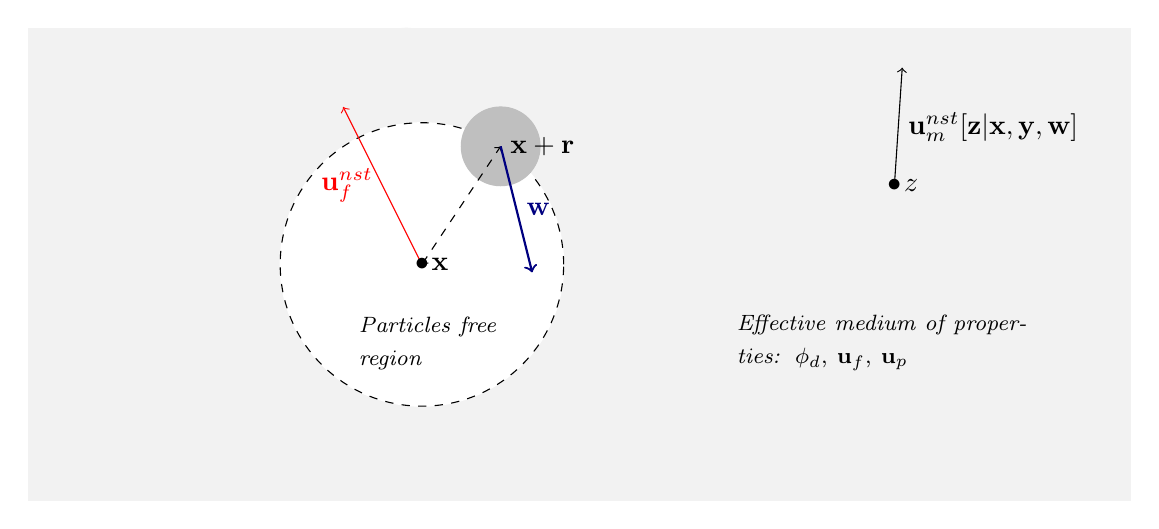
\begin{tikzpicture}
    \filldraw[gray!10](-5,-3) rectangle(9,3);
    \filldraw[white](0,0) circle (1.8);
    \filldraw[ gray!10!white](+2.6,0.5)circle (0.5);
    \filldraw[ gray!10!white](-1.5,2.2)circle (0.5);
    \draw[dashed](0:1.8) arc (0:360:1.8);
    % \filldraw[ gray!50!white](0,0) circle (0.5);
    \filldraw[ gray!50!white](1,1.5)circle (0.5);
    \filldraw[ gray!10!white](-0.2,2.5)circle (0.5);
    \draw[->,red](0,0)--++(-1,2)node[midway,left]{$\textbf{u}_f^\text{nst}$};
    \draw(0,0)node{$\bullet$}node[right]{$\textbf{x}$};
    \draw[dashed,<->](0,0)--(1,1.5)node[right]{$\textbf{x}+\textbf{r}$};
    \draw[->,blue!50!black,thick](1,1.5)--++(0.4,-1.6)node[midway,right]{$\textbf{w}$};
    % \draw[dashed](-0.2,3.5);
    \node[text width=2cm] (title) at (0.2,-1) {\footnotesize\textit{Particles free region}};
    % \node[ultra thick] (title) at (-0.5,-1.5) {(\textit{Case 1})};
    \node[text width=4cm] (title) at (6,-1) {\footnotesize\textit{Effective medium of properties:} $\phi_d$, $\textbf{u}_f$, $\textbf{u}_p$};
    \draw[->] (6,1)node{$\bullet$}node[right]{$z$}--++(0.1,1.5)node[right,midway]{$\textbf{u}_m^\text{nst}[\textbf{z}|\textbf{x},\textbf{y},\textbf{w}]$};
\end{tikzpicture} 
\caption{Representation of the \textit{nearest neighbor conditionally averaged} velocity fields $\textbf{u}_\text{nst}^f[\textbf{x},\textbf{w},\textbf{r},t]$, Inspired from (Figure 2) of \citet{zhang2021ensemble}}
\label{fig:unst}
\end{figure}
According to \ref{eq:def_f_nst} and \ref{fig:unst} $\textbf{u}_f^\text{nst}[\textbf{x},\textbf{r},\textbf{w}]$ is the averaged value of $\textbf{u}_f^0$, evaluated at \textbf{x}, on all configuration where a particle is present at $\textbf{y} = \textbf{x} + \textbf{r}$ with velocity $\textbf{w}$. 
Consequently, the region delimited by the sphere, centered at \textbf{x} of radius $|\textbf{y} - \textbf{x}|$ must be empty of particles center of mass \citep{zhang2021ensemble}. 
This deeper physical understanding will prove valuable in the subsequent section.  



\subsection{How to obtain the nearest neighbor conditional velocity fields ?}

In the objective of computing the sedimentation velocity, \citet[Appendix B]{zhang2021ensemble} has computed $\textbf{u}_f^\text{nst}$ using the \textit{nearest neighbor conditional averaged} Navier-Stokes equations. 
As his derivation does not provide detailed proof, especially on the derivation of Equation (B 1) of \citet{zhang2021ensemble},  we aim in this section to present a broader methodology. 

Inspired by the classic conditional average method of \citet{hinch1977averaged}, we stipulate that the nearest neighbor conditional velocity fields, i.e. $\textbf{v}_f^\text{nst}$,can be obtained by conditionally averaging the local scale mass and momentum equations, and solve for $\textbf{v}_f^\text{nst}$. 
Thus, let us first recall the local mass and momentum equation, 
\begin{align}
    \pddt (\rho_f\chi_f) +  \pddx \cdot (\rho_f\chi_f\textbf{u}^0_f) &= 0 \\
    \pddt (\rho_f\chi_f\textbf{u}^0_f)
    + \pddx\cdot (\rho_f\chi_f\textbf{u}^0_f\textbf{u}^0_f - \chi_f\bm\sigma^0_f)
    &= 
    - \delta_\Gamma \bm\sigma_f^0 \cdot \textbf{n}_d. 
    + \chi_f \rho_f \textbf{g}
    \label{eq:local_equations}
\end{align}
Then, note that we can obtain $\textbf{v}_f^\text{nst}$ from $\textbf{u}_f^0$ directly by the operation, 
\begin{equation*}
    \textbf{v}_f^\text{nst} P_\text{nst}^f
    = 
    \textbf{u}_f^\text{nst} P_\text{nst}^f
    - \textbf{u}_f P_\text{nst}^f
    = 
    \avg{\delta_\text{nst}^f \chi_f \textbf{u}_f^0}
    - \textbf{u}_f P_\text{nst}^f
\end{equation*}
We deduce that to obtain an equation for $\textbf{u}_f^\text{nst}$ we must multiply, \ref{eq:local_equations} by $\delta_\text{nst}$ and average overall configurations. 
This introduces the need of proper conservation equation for $\delta_\text{nst}$. 

\subsubsection{Conditionally mass transport equation}
Consequently, we introduce the  conservation equation of each distribution present in $\delta_\text{nst}$, it reads, 
\begin{align}
    \label{eq:dt_delta_x}
    \pddt \delta(\textbf{x}_i  - \textbf{y})
    +\textbf{u}_i  
    \cdot \pddy \delta(\textbf{x}_i  - \textbf{y})
    = 0\\
    \pddt \delta(\textbf{u}_i -\textbf{w})
    +\textbf{a}_i \cdot  \pddw   \delta(\textbf{u}_i  - \textbf{w})
    = 0\\
    \pddt \chi_f 
    + \textbf{u}_\Gamma^0 
    \cdot \pddx \chi_f = 0 \\
    \pddx \chi_f = - \delta_\Gamma \textbf{n}_f,
    \label{eq:chi_f_dt}
\end{align}
where we recall that $\textbf{u}_\Gamma^0$ is the velocity of the droplets interfaces, and $\textbf{n}_f$ is the normal pointing inward the droplets surfaces. 
Additionally, The vector $\textbf{a}_i$ correspond to the center of mass acceleration of the particle $i$. 
Form \ref{eq:dt_delta_x} to \ref{eq:chi_f_dt} we deduce that, 
\begin{align}
    \pddt \delta_\text{nst}
    + \pddy \cdot (\textbf{w} \delta_\text{nst})
    + \pddw \cdot (\textbf{a}_i  \delta_\text{nst})
    = 
    \sum_i \delta(\textbf{x}_i -\textbf{y}) \delta(\textbf{u}_i - \textbf{w}) \pddt h_i
\end{align}
% and, 
% \begin{align*}
%     \pddt (\chi_f \delta_\text{nst})
%     + \pddy \cdot (\textbf{w} \chi_f \delta_\text{nst})
%     + \pddw \cdot (\textbf{a}_i  \chi_f \delta_\text{nst})
%     = 
%     \chi_f \delta(\textbf{x}_i -\textbf{y}) \delta(\textbf{u}_i - \textbf{w}) \pddt h_i
%     + \delta_\Gamma \delta_\text{nst} \textbf{u}_\Gamma\cdot \textbf{n}_f
% \end{align*}
As, shown in appendix, 
\begin{align}
    \pddt  h_i[\textbf{x},t,\FF]
    = 
    h_i
    \sum_k 
    \delta(r_k - r_i)
    (\textbf{u}_k  \cdot \hat{\textbf{r}}_k - \textbf{u}_i  \cdot \hat{\textbf{r}}_i)\\
    \pddx  h_i[\textbf{x},t,\FF]
    = 
    h_i
    \sum_k 
    \delta(r_k - r_i)
    ( \hat{\textbf{r}}_k -  \hat{\textbf{r}}_i),
\end{align}
where we recall that $\textbf{u}_k$ and $\textbf{u}_i$  are the center of mass velocity of the particle $k$ and $i$ respectively.
Note that the second expression is in agreement with \citet[Appendix A]{zhang2021ensemble}. 
We also introduced the radial distance from the particle $i$ to the point $\textbf{x}$ namely, $r_i = |\textbf{x}_i - \textbf{x}|$.  
Anyhow, considering this relation yields a new expression for the transport equation of $\delta_\text{nst}$ namely,
\begin{equation}
    \pddt \delta_\text{nst}
    + \pddy \cdot (\textbf{w} \delta_\text{nst})
    + \pddw \cdot (\textbf{a}_i  \delta_\text{nst})
    = 
    % \sum_i
    % \delta(\textbf{x}_i -\textbf{y}) 
    % \delta(\textbf{u}_i - \textbf{w}) 
    \delta_\text{nst}
    % h_i
    \sum_k 
    \delta(r_k - r_i)
    (\textbf{u}_k  \cdot \hat{\textbf{r}}_k - \textbf{u}_i  \cdot \hat{\textbf{r}}_i). 
    % \label{eq:dt_delta_nst}
\end{equation}
As demonstrated in \citet{zhang2023evolution}, in another context, the right-hand side term of \ref{eq:dt_delta_nst} can be considered as a source term due to the birth or death of nearest neighbor to the point \textbf{x}. 
For reason that will become clear latter on we add the term $\textbf{u}_f^0\cdot \pddx \delta_\text{nst}$ on each side of the equation, which gives,
\begin{equation}
    \pddt \delta_\text{nst}
    + \textbf{u}_f^0\cdot \pddx \delta_\text{nst}
    + \textbf{w}   \cdot \pddy \delta_\text{nst}
    + \textbf{a}_i \cdot \pddw   \delta_\text{nst}
    = 
    % \sum_i
    % \delta(\textbf{x}_i -\textbf{y}) 
    % \delta(\textbf{u}_i - \textbf{w}) 
    \delta_\text{nst}
    % h_i
    \sum_k 
    \delta(r_k - r_i)
    ((\textbf{u}_k - \textbf{u}_f^0) \cdot \hat{\textbf{r}}_k - (\textbf{u}_i  - \textbf{u}_f^0)\cdot \hat{\textbf{r}}_i). 
    \label{eq:dt_delta_nst}
\end{equation}
On the right-hand side we have reformulated the term $\textbf{u}_f^0\cdot \pddx \delta_\text{nst}$, see \tb{Annexe} for the full derivation. 

To derive an equation for $P_\text{nst}^f$ we multiply \ref{eq:dt_delta_nst} by $\chi_f$, and make use of \ref{eq:chi_f_dt}, yielding, 
\begin{multline}
    \pddt (\chi_f\delta_\text{nst})
    +  \pddx \cdot (\textbf{u}_f^0 \chi_f\delta_\text{nst})
    +  \pddy \cdot (\textbf{w}    \chi_f\delta_\text{nst})
    +  \pddw \cdot   (\textbf{a}_i  \chi_f\delta_\text{nst})\\
    = 
    % \sum_i
    % \delta(\textbf{x}_i -\textbf{y}) 
    % \delta(\textbf{u}_i - \textbf{w}) 
    (\chi_f\delta_\text{nst})
    % h_i
    \sum_k 
    \delta(r_k - r_i)
    ((\textbf{u}_k - \textbf{u}_f^0) \cdot \hat{\textbf{r}}_k - (\textbf{u}_i  - \textbf{u}_f^0)\cdot \hat{\textbf{r}}_i). 
    \label{eq:dt_delta_nst_f}
\end{multline}
which upon averaging gives directly,
\begin{multline}
    \pddt (\phi_fP_\text{nst}^f)
    + 
    \pddx \cdot (
        \phi_f 
        P_\text{nst}^f
        \textbf{u}_f^\text{nst}
    )
    + \pddy \cdot (
        \phi_f
        P_\text{nst}^f
        \textbf{w} 
    )
    +
    \pddw \cdot (  
        \phi_f 
        P_\text{nst}^f
        \textbf{a}_p^\text{nst} 
    )
    = \\
    + \avg{
    %  \chi_f \textbf{u}_\Gamma \cdot \pddx \delta_\text{nst}
     \chi_f \delta_\text{nst}
    \sum_k 
    \delta(r_k - r_i)
    [(\textbf{u}_k - \textbf{u}_\Gamma^0) \cdot \hat{\textbf{r}}_k - (\textbf{u}_i- \textbf{u}_\Gamma^0)  \cdot \hat{\textbf{r}}_i]}.
    \label{eq:dt_P_nst_chi}
\end{multline}
where we have noticed that $\textbf{u}_\Gamma^0 = \textbf{u}_f^0$ in the absence of mass transfer. 
In this relation the left-hand side terms represent the advection of $\phi_f P_\text{nst}^f$.
The source term on the right-hand side of \ref{eq:dt_delta_nst_chi} accounts for the changes in nearest neighbor distribution due to the permutation of the nearest neighbor at the local scale. 
Notice the similarities of the right-hand side source term of \ref{eq:dt_delta_nst_chi} with (A10) of \citet{zhang2023evolution}, which derived a transport equation for $P_\text{nst}$ such as it is defined in the previous chapters. 
We remark that the source terms of (A10) and \ref{eq:dt_delta_nst_chi} yield the same form, but in \ref{eq:dt_delta_nst_chi} the velocity $\textbf{u}_i$ and $\textbf{u}_k$ are evaluated with respect to the local velocity of the fluid $\textbf{u}_f^0$, while in \citet{zhang2023evolution} it is evaluated relative to the velocity of the particles centered at \textbf{x}. 
This is not surprising considering the difference in definition between $P_\text{nst}^f$ and $P_\text{nst}$ in \citet{zhang2023evolution}. 


\ref{eq:dt_P_nst_chi} which can also be written in ``conservative'' form using \ref{eq:dt_P_nst_chi} and, 
\begin{equation}
    \pddt \phi_f 
    + \div(
        \phi_f
        \textbf{u}_f 
        ) 
    = 0, 
\end{equation}
to show that \ref{eq:dt_delta_nst_chi} can be written in ``conservative'' form, yielding, 
\begin{multline}
    \pddt P_\text{nst}^f
    + 
    \pddx \cdot (
        P_\text{nst}^f
        \textbf{u}_f^\text{nst}
    )
    + \pddy \cdot (
        P_\text{nst}^f
        \textbf{w}
    )
    +
    \pddw \cdot (  
        P_\text{nst}^f
        \textbf{a}_p^\text{nst} 
    )
    = \\
    + \frac{1}{\phi_f}\avg{
    %  \chi_f \textbf{u}_\Gamma \cdot \pddx \delta_\text{nst}
     \chi_f \delta_\text{nst}
    \sum_k 
    \delta(r_k - r_i)
    [(\textbf{u}_k - \textbf{u}_\Gamma^0) \cdot \hat{\textbf{r}}_k - (\textbf{u}_i- \textbf{u}_\Gamma^0)  \cdot \hat{\textbf{r}}_i]}.
    \label{eq:dt_Pc_nst_chi}
\end{multline}
This equation multiplied by $\rho_f$ corresponds to the \textit{nearest neighbor conditional averaged} mass equation of the fluid phase. 

\subsubsection{First form of the conditional averaged momentum equaiton}
Now that the transport equation for $\delta_\text{nst}$ and $P_\text{nst}^f$ are properly derived we are able to derive the \textit{nearest neighbor conditionally averaged} momentum equation. 
Multiplying \ref{eq:local_equations} by $\delta_\text{nst}$ , making use of \ref{eq:dt_delta_nst} and averaging overall configurations yields, 
\begin{multline}
    \pddt (\rho_f\phi_f P_\text{nst} \textbf{u}^\text{nst}_f)
    + \pddx\cdot (
        \rho_f\phi_fP_\text{nst}^f \textbf{u}^\text{nst}_f\textbf{u}^\text{nst}_f 
        +\bm\sigma_\text{nst}^\text{eq})
    + \pddy\cdot (\phi_fP_\text{nst}^f \textbf{w}\textbf{u}_f^\text{nst} )
    + \pddw\cdot (\phi_fP_\text{nst}^f \textbf{a}_p^\text{nst} \textbf{u}_f^\text{nst} )\\
    = 
    \phi_fP_\text{nst}^f  \rho_f \textbf{g}
    - \avg{\delta_\text{nst}\delta_\Gamma \bm\sigma_f \cdot \textbf{n}_d} 
    % - \avg{\chi_f \bm\sigma_f^0 \cdot \grad\delta_\text{nst}}
    +\avg{
        \delta_\text{nst}
        \chi_f \bm\sigma_f^0 \cdot
        \sum_k 
        \delta(r_k - r_i)
        [\hat{\textbf{r}}_k - \hat{\textbf{r}}_i]}\\
    +\avg{
        %  \chi_f \textbf{u}_\Gamma \cdot \pddx \delta_\text{nst}
         \textbf{u}_f^0\chi_f \delta_\text{nst}
        \sum_k 
        \delta(r_k - r_i)
        [(\textbf{u}_k - \textbf{u}_f^0) \cdot \hat{\textbf{r}}_k - (\textbf{u}_i- \textbf{u}_f^0)  \cdot \hat{\textbf{r}}_i]},
    \label{eq:momentum_avg_nst}
\end{multline}
with the effective stress $\bm\sigma_\text{nst}^\text{eq}$ defined as, 
\begin{equation}
    \bm\sigma_\text{nst}^\text{eq}=
    \avg{\rho_f\chi_f\delta_\text{nst} \textbf{u}''_f\textbf{u}''_f} 
    - \phi_f P_\text{nst}^f \bm\sigma^\text{nst}_f. 
\end{equation}
The terms on the left-hand side of \ref{eq:momentum_avg_nst} represents the advection of the \textit{nearest neighbor conditional average} momentum along the phase space coordinate, plus the contribution of the \textit{nearest neighbor conditional average} viscous stresses $\bm\sigma^\text{nst}_f$
The first term on right-hand side of \ref{eq:momentum_avg_nst} corresponds to the momentum exchange between phases, but conditionally averaged. 
The second and third terms are the additional contribution of the convective and non-convective fluxes due to the birth or death of nearest neighbors. 

In this form \ref{eq:momentum_avg_nst} is hardly solvable. 
Although boundary condition are available at the surface of our particle, for the velocity $\textbf{u}_f^\text{nst}[\textbf{y}+a \textbf{n}, \textbf{y},\textbf{w}]$ there is a lake of boundary condition infinitely far from the particle. 
Indeed, in this form $\lim_{|\textbf{x}- \textbf{y}|\to \infty} \textbf{u}^\text{nst}_f = \text{Undefined}$ because in the same limits $P_\text{nst}^f = 0$. 

\subsubsection{Second form of the conditional averaged equation}

To settle this issue we follow \citet[Appendix B]{zhang2021ensemble} and propose to solve for an auxiliary problem which is equivalent to the conservation equation of $\textbf{u}_f^\text{nst}[\textbf{x},\textbf{y},\textbf{w},t]$. 
We introduce the conditionally averaged fields, 
\begin{equation*}
    P_\text{nst}^f[\textbf{y},\textbf{w},\textbf{x},t]\textbf{u}^\text{nst}[\textbf{z},t|\textbf{x},\textbf{y},\textbf{w}]
    = \avg{\delta_\text{nst}^f  \textbf{u}^0[\textbf{z},\FF,t]}
    \label{eq:def_u_z}
\end{equation*}
where, $\delta_\text{nst}^f = \chi_f[\textbf{x},t,\FF]\delta_\text{nst}[\textbf{y},\textbf{w}, \FF,t]$. 
Additionally, we modified slightly the definition of $P_\text{nst}^f$, such that our new definition  is $\phi_f$ times the previous definition made in the preceding section, $P_\text{nst}^f[\textbf{x},\textbf{y},\textbf{w},t] = \phi_f[\textbf{x},t]P_\text{nst}^f[\textbf{y},\textbf{w},t|\textbf{x}]$. 
% With that definition, $\phi_f^\text{nst}$ is the fluid \textit{nearest neighbor conditionally averaged} fluid phase volume fraction, such that $\phi_f^\text{nst}$ represents the fluid phase volume fraction evaluated at \textbf{z} averaged on all configurations where \textbf{x} is occupied by the fluid phase and $\textbf{y}$ by a particle center of mass, with velocity $\textbf{w}$.  
$\textbf{u}^\text{nst}$ is the \textit{nearest neighbor conditionally averaged} velocity evaluated at $\textbf{z}$, knowing the fluid phase is also present at $\textbf{x}$ with the nearest neighbor to \textbf{x} being located in \textbf{y} with velocity \textbf{w}. 
A graphical representation of $\textbf{u}^\text{nst}$ is given \ref{fig:unst}.
With that definition we have the following boundary condition far from the particle free region, 
\begin{align*}
    \lim_{|\textbf{z} - \textbf{y}|\to \infty}
    \textbf{u}^\text{nst}[\textbf{z},t|\textbf{x},\textbf{y},\textbf{w}]
    = \textbf{u}[\textbf{z},t]
    % \lim_{|\textbf{z} - \textbf{y}|\to \infty}
    % \phi^\text{nst}[\textbf{z},t|\textbf{x},\textbf{y},\textbf{w}]
    % = \phi[\textbf{z},t],
    \label{eq:boundary}
\end{align*}
since far from the particle free region the effect of the particle located at \textbf{y} has no impact on the averaged quantities. 
Thus, $\textbf{u}^\text{nst}$ has the advantage of having proper boundary condition at infinity and is related to $\textbf{u}_f^\text{nst}$ such that, $\textbf{u}^\text{nst}[\textbf{x},t|\textbf{x},\textbf{y},\textbf{w}] = \textbf{u}_f^\text{nst}[\textbf{x},t|\textbf{y},\textbf{w}]$ since only the fluid phase is present at \textbf{x} by definition of $\textbf{u}^\text{nst}$. 

We also introduce the disturbance fields $\textbf{v}^\text{nst} = \textbf{u}^\text{nst} - \textbf{u}$, which follows the condition at infinity, 
\begin{equation}
    \lim_{|\textbf{z} - \textbf{y}|\to \infty}
    \textbf{v}^\text{nst}[\textbf{z},t|\textbf{x},\textbf{y},\textbf{w}]
    = 0,
\end{equation}
while the boundary condition at the surface of the particle is given by, 
\begin{equation}
    \textbf{v}^\text{nst}\cdot \textbf{n}
    = 
    (\textbf{w} - \textbf{u}[\textbf{z},t])\cdot \textbf{n}
    = 
    \left\{
        \textbf{w}
        - \textbf{u}
        - (\textbf{y} - \textbf{z})\cdot \grad\textbf{u}
        + \ldots 
    \right\}
    \;\;\; \forall \textbf{z}\in \left\{ |\textbf{z} - \textbf{y}| = a  \right\}. 
    \label{eq:bounday2}
\end{equation}
Notice that these boundaries conditions and the one derived in \ref{chap:daniel2} for the \textit{Single-point conditionally averaged} Navier-Stokes equations  are exactly the same but applied on the bulk velocity rather than on the continuous phase velocity.

Instead of using the fluid phase formulation of the mass and momentum local conservation equations, \eqref{eq:local_equations}, we use the \textit{single-fluid}, mass and momentum equations, namely, 
\begin{align}
    \pddz \cdot \textbf{u}^0 = 0 \\
    \pddt (\rho^0\textbf{u}^0_f)
    + \pddz\cdot 
    (\rho^0\textbf{u}^0\textbf{u}^0 
    -\bm\sigma^0)
    &= 
    + \rho^0 \textbf{g}. 
    \label{eq:local_equations_bulk}
\end{align}
Multiplying these equations by $(\delta_\text{nst}^f - P_\text{nst}^f)$ and averaging overall configurations yields the Navier-Stokes equations for the distance fields $\textbf{v}^\text{nst}$, namely,
\begin{equation}
    \pddz \cdot \avg{(\delta_\text{nst}^f - P_\text{nst}^f) \textbf{u}^0}
    = 0,
    \label{eq:mass_nst_d}
\end{equation}
and,
\begin{multline}
    \pddt \avg{(\delta_\text{nst}^f - P_\text{nst}^f)\rho^0\textbf{u}^0}
    + \pddz\cdot \avg{ (\delta_\text{nst}^f - P_\text{nst}^f) ( \rho^0  \textbf{u}^0 \textbf{u}^0 - \bm\sigma^0)}\\
    +  \pddx \cdot \avg{(\delta_\text{nst}^f \textbf{u}_f^0 - P_\text{nst}^f\textbf{u}_f^\text{nst}) \rho^0 \textbf{u}^0}
    +  \pddy \cdot \avg{(\delta_\text{nst}^f - P_\text{nst}^f) \textbf{w} \textbf{u}^0 \rho^0}
    +  \pddw \cdot \avg{(\delta_\text{nst}^f \textbf{a}_i - P_\text{nst}^f \textbf{a}_p^\text{nst})\textbf{u}^0 \rho^0 }\\
    = 
    % - \avg{(\delta_\text{nst}^f - P_\text{nst}^f)\delta_\Gamma \bm\sigma_f^0 \cdot \textbf{n}_d }
    + \avg{(\delta_\text{nst}^f - P_\text{nst}^f)\rho^0 \textbf{g}} 
    + 
    \avg{\rho^0 \textbf{u}^0 S'_\text{nst} },
    \label{eq:momentum_nst_d}
\end{multline}
where we have defined $S_\text{nst}'$ as the source term due to the interchanges of the nearest particles,
\begin{multline}
    S_\text{nst}'
    =
    \left\{
    \delta_\text{nst}^f
        % h_i
        \sum_k 
        \delta(r_k - r_i)
        ((\textbf{u}_k - \textbf{u}_f^0) \cdot \hat{\textbf{r}}_k - (\textbf{u}_i  - \textbf{u}_f^0)\cdot \hat{\textbf{r}}_i) 
    - \right.\\ \left.
    \avg{
         \delta_\text{nst}^f
        % h_i
        \sum_k 
        \delta(r_k - r_i)
        ((\textbf{u}_k - \textbf{u}_f^0) \cdot \hat{\textbf{r}}_k - (\textbf{u}_i  - \textbf{u}_f^0)\cdot \hat{\textbf{r}}_i) 
    }
    \right\}. 
\end{multline}
In this quite general form these equations may seem complicated, therefore let us describe in details the meaning of each term. 
We start by the conditional ``mass'' conservation equation \eqref{eq:mass_nst_d}. 
The term within the divergence sign can be written,  
\begin{equation}
    \avg{(\delta_\text{nst}^f - P_\text{nst}^f )\textbf{u}^0}
    = P_\text{nst}^f (\textbf{u}^\text{nst} - \textbf{u})
    = P_\text{nst}^f \textbf{v}^\text{nst}
\end{equation}
Since $P_\text{nst}$ is not a function of \textbf{z}, we have shown that $\textbf{v}^\text{nst}$ is divergence free, regardless of the flow regime. 

Regarding the \textit{nearest neighbor conditionally averaged} equations \eqref{eq:momentum_nst_d} we may reformulate the first term on the right-hand side such as, 
\begin{equation}
    \avg{(\delta_\text{nst}^f - P_\text{nst}^f)\rho^0 \textbf{u}^0}
    = P_\text{nst}^f [
        \rho^\text{nst}\textbf{u}_m^\text{nst}
        - 
        \rho \textbf{u}_m
    ]
    = P_\text{nst}^f [
        \rho^\text{nst-d}\textbf{v}^\text{nst}_m
        + \rho^\text{nst-d}\textbf{u}_m
        + \rho \textbf{v}^\text{nst}_m
    ]
\end{equation}
where we recall that $\rho \textbf{u}_m = \avg{\rho_f\chi_f \textbf{u}_f + \rho_d\chi_f  \textbf{u}_d}$ is the weighted or Favre average.
We introduced the superscript $-d$ on $\rho^\text{nst-d}$ to denote the \textit{disturbance} since $\phi_f^\text{nst-d}$ is a disturbance field that vanish at large $\textbf{z}$ according to \ref{eq:boundary}. 
Therefore, \ref{eq:momentum_nst_d} is an equation of conservation for the disturbance velocity field generated by the droplet at \textbf{y} which is the nearest neighbor to a point \textbf{x} in the fluid phase. 
The remaining terms on the left-hand side of \ref{eq:momentum_avg_nst} correspond to the advective terms over the phase space coordinate, plus the \textit{nearest neighbor conditionally averaged } disturbance viscous stress, namely, 
\begin{equation}
    \avg{(\delta_\text{nst}^f - P_\text{nst}^f) \bm\sigma^0}
    = P_\text{nst} \bm\sigma^\text{nst}
\end{equation}
Note that since both fluids are considered Newtonian $\bm\sigma_k^0 = -p_k^0\bm\delta + \mu_k (\grad \textbf{u}_k^0 + \grad \textbf{u}_k^0)$, therefore,
\begin{align}
    \avg{(\delta_\text{nst}^f - P_\text{nst}^f) \bm\sigma^0}
    &=
    \avg{(\delta_\text{nst}^f - P_\text{nst}^f) 
    \left[
    - p^0 \bm\delta 
    + \mu_f(\grad \textbf{u}^\dagger + (\grad \textbf{u}^0)^\dagger )
    + \chi_d (\mu_d-\mu_f)\textbf{e}_d^0 
    + \delta_\Gamma \gamma (\bm\delta - \textbf{nn})
    \right]
    }\nonumber \\
    &=
    P_\text{nst}^f\left\{
        -p^\text{nst-d}\bm\delta 
        + \mu_f [\pddz \textbf{u}^\text{nst-d}+^\dagger\pddz \textbf{u}^\text{nst-d}]
    \right\}\nonumber\\
   &+  \avg{(\delta_\text{nst}^f - P_\text{nst}^f)[
    \chi_d  2 (\mu_d-\mu_f)\textbf{e}_d^0 
    + \delta_\Gamma \gamma (\bm\delta - \textbf{nn})]
    }
\end{align}
Where the term on the last line is the conditional stress contribution from the particle phase compared to the mean particle contribution to the stress. 
This stress also satisfy the property to vanish at large distance to the particle-free zone.

On the right-hand side of \ref{eq:momentum_nst_d} we recover the ``disturbance source terms'' one of which is the Buoyancy force, but conditionally averaged, namely, 
\begin{equation*}
    \avg{(\delta_\text{nst} - P_\text{nst}^f) \chi_f \rho^0 \textbf{g}}
    = 
    P_\text{nst}^f \rho^\text{nst-d} \textbf{g}. 
\end{equation*}
The momentum source due to exchange with the disperse phase can be express in the same way. 
The last term on the right-hand side also corresponds to the change of momentum generated by changes of nearest neighbors to \textbf{x}. 
\tb{explain the meaning of $\rho^\text{nst-d}$ }

To summary \ref{eq:mass_nst_d} and \ref{eq:momentum_nst_d} together with the boundary conditions formed by \ref{eq:boundary} and \ref{eq:bounday2}, constitute a system of conditionally averaged equation, to be solved for the disturbance velocity fields, $\textbf{v}^\text{nst}[\textbf{z},t|\textbf{x},\textbf{y},\textbf{w}]$ and the disturbance density, $\rho^\text{nst-d}[\textbf{z},t|\textbf{x},\textbf{y},\textbf{w}]$.
However, due to the complexity of the problem, arising due to the consideration of a phase space with  13 dimension ($\textbf{z},t,\textbf{x},\textbf{y},\textbf{w}$), we must now consider some simplifying hypothesis.

\subsection{Simplifying assumptions}

Due to the challenging theoretical aspect of the problem we must now, take some simplifying hypotheses that are not rigorous. 
Indeed, from now on we consider these unfounded assumptions :
% At this stage we must perform some restrictive assumptions in order to make theoretical advancement. 
Firstly, we consider a stationary, inertialess problem, implying that we neglect the time derivatives and advective terms in \ref{eq:mass_nst_d} and \ref{eq:momentum_nst_d}. 
Indeed, under this form the advective terms are all proportional to $\textbf{v}^\text{nst}\textbf{v}^\text{nst}$, which is itself proportional to the relative velocity between the particle and the continuous phase. 
Therefore, these terms are of $\mathcal{O}(Re)$ or higher, with $Re$ is the Reynolds number based on the relative phase velocity.

Likewise, we will consider the dilute regime meaning that we neglect all the terms of $\mathcal{O}(\phi)$ or higher. 
And finally, we will consider that the suspension is homogeneous, such that the ensemble averaged quantities are uniform, meaning that they are not function of $\textbf{z}$. 


Regarding the density disturbance fields, $\rho^\text{nst-d}$, we assume the following form in the dilute regime, 
\begin{equation*}
    \rho^\text{nst-d}[\textbf{z},t|\textbf{x},\textbf{y},\textbf{w}]
    = \phi_d (\rho_f - \rho_d) H(|\textbf{y} - \textbf{x}| - |\textbf{z} - \textbf{x}|)
\end{equation*}
Meaning that in the particle free-region $\rho^\text{nst} = \rho_f$ and outside the particle free region $\rho^\text{nst} = \phi_d\rho_d + \phi_f\rho_f= \rho$, since we consider the values of the effective medium outside this region \ref{fig:unst}. 
Notice that this definition applies only to the points \textbf{z} exterior to the particle since inside the particle we consider the classic stokes equations. 
Thus, the buoyancy source term is given by, 
\begin{equation*}
    \avg{(\delta_\text{nst} - P_\text{nst}^f) \chi_f \rho_f \textbf{g}}
    = 
    P_\text{nst}^f [\textbf{x},\textbf{y},\textbf{w},t]
    \phi_d[\textbf{z},t] 
    \textbf{g}
    (\rho_f - \rho_d) H(|\textbf{y} - \textbf{x}| - |\textbf{z} - \textbf{x}|), 
\end{equation*}
outside the particle domain. 
Where we made explicit the dependency of each variable, to point-out the fact that for example in a uniform and steady-state medium $\phi_d[\textbf{z},t] = \phi$ is constant. 
Again in these definitions applies only to the point \textbf{z} outside the particle how's center is located at \textbf{y}. 

At this stage the source term $S_\text{nst}'$ is hard to model however it seems that it is negligible at $\mathcal{O}(\phi)$ \citet{zhang2021ensemble}. 
Indeed, this term is non-zero only when a second-nearest neighbor is present, meaning that it is proportional to a pairs' probability density which is or order $\phi$ higher than the other terms. 
It seems also reasonable to neglect the particle contribution to the bulk stress as this terms becomes of $\mathcal{O}(\phi^2)$, thus we may write, 
\begin{equation}
    \avg{(\delta_\text{nst}^f - P_\text{nst}^f) \bm\sigma^0}
    =
    P_\text{nst}^f\left\{
        -p^\text{nst-d}\bm\delta 
        + \mu_f [\pddz \textbf{u}^\text{nst-d}+^\dagger\pddz \textbf{u}^\text{nst-d}]
    \right\}
\end{equation}
The particle contribution to the suspension stress may be written in this case, 
\begin{align}
    {\chi_d  2 (\mu_d-\mu_f)\textbf{e}_d^0 
    + \delta_\Gamma \gamma (\bm\delta - \textbf{nn})}
    &\approx
    \frac{1}{2}
     \intS{
        \left[(\textbf{r}\bm\sigma_f^0 
        + \bm\sigma_f^0 \textbf{r}
        - \frac{2}{3}\bm\sigma_f^0 \cdot \textbf{r}
        )\cdot \textbf{n} 
        - 2\mu_f (
            \textbf{u}_f^0 \textbf{n}
            + \textbf{n}\textbf{u}_f^0 
        )\right]
    }
    % \nonumber\\
    % &- \pddz \cdot \left[
    %     \intS{
    %     \textbf{rr}(\bm\sigma_f^0 \cdot \textbf{n} )}
    %     - 2\mu_f\intO{\textbf{re}_d^0}
    % \right]
\end{align}
where we have neglected the higher order moments and considered $\chi_d = \delta_p v_\alpha$. 
Notice that this corresponds exactly to the Stresslet quantity. 
According to \ref{fig:unst} we can assume that, 
\begin{align}
    &\avg{(\delta_\text{nst}^f - P_\text{nst}^f)[\chi_d  2 (\mu_d-\mu_f)\textbf{e}_d^0 
    + \delta_\Gamma \gamma (\bm\delta - \textbf{nn})]}\nonumber \\
    &\approx
    -\frac{1}{2}
     \pSavg{
        \left[(\textbf{r}\bm\sigma_f^0 
        + \bm\sigma_f^0 \textbf{r}
        - \frac{2}{3}\bm\sigma_f^0 \cdot \textbf{r}
        )\cdot \textbf{n} 
        - 2\mu_f (
            \textbf{u}_f^0 \textbf{n}
            + \textbf{n}\textbf{u}_f^0 
        )\right]
    }
    H(|\textbf{y}- \textbf{x}| - |\textbf{z} -\textbf{x}|)\nonumber \\
    &= -\textbf{S}_p[\textbf{z},t]
    H(|\textbf{y}- \textbf{x}| - |\textbf{z} -\textbf{x}|)
    % \nonumber\\
    % &- \pddz \cdot \left[
    %     \intS{
    %     \textbf{rr}(\bm\sigma_f^0 \cdot \textbf{n} )}
    %     - 2\mu_f\intO{\textbf{re}_d^0}
    % \right]
\end{align}
where we considered that the \textit{nearest neighbor averaged} Stresslet where zero in the particle free zone and that it takes the value of the ensemble averaged stresslet $\textbf{S}_p$ outside the particle free zone.
We therefore neglected the particle-partcile interactions and the influence of the details of the flow on this contribution. 
It is clear that, $\textbf{S}_p \sim \textbf{e}$, here we do not consider the mean shearing motion therefore this contribution can be neglected. 
\tb{however the moment of order two might be accounted for  ! !! ! ! ! }

Considering all of these hypotheses we may re-write the mass and momentum conditionally averaged equations of the bulk phases on the domain outside the particle at \textbf{y}, as follows,
\begin{equation}
    % \pddt \avg{(\delta_\text{nst}^f - P_\text{nst}^f)\chi_f}
    \pddz \cdot \textbf{v}^\text{nst}
    = 0
    \label{eq:mass_nst_d_stokes}
\end{equation}
\begin{equation}
    - \pddz p^\text{nst-d} 
    + \mu_f \pddz^2 \textbf{u}^\text{nst-d}
    = 
    \phi
    \textbf{g}
    (\rho_f - \rho_d) H(|\textbf{y} - \textbf{x}| - |\textbf{z} - \textbf{x}|)
    \label{eq:momentum_nst_d_stokes}
\end{equation}
In summary, following our rigorous averaging method we demonstrated that $\textbf{v}^\text{nst}$ followed the forces Stokes equations. 
This equation are in agreement with \citet{zhang2021ensemble} how provided no proof for his derivation. 
Additionally, \citet{zhang2021ensemble} carried the derivation for $\textbf{u}^\text{nst}$ and not $\textbf{v}^\text{nst}$, this is the reason why an additional uniform source term is present on the left-hand side of his Equation (B 1). 
While this difference seems a detail, it is of major importance since only the disturbance fields $\textbf{v}^\text{nst}$ follows the Stokes equations in the general case, not $\textbf{u}^\text{nst}$. 
Indeed, the latter include the macroscopic fields $\textbf{u}$ how follow in general the Navier-Stokes equations including the inertial terms. 

We argue however that the particle free-zone as defined by \citep{zhang2021ensemble} is incomplete. 
Indeed, inside the spherical shell of radius $2a$ centered at $\textbf{y}$ no center of mass of particle is found due to the impenetrability of the droplets. 
Thus, to be consistent the right-hand side of \ref{eq:momentum_nst_d_stokes} must be modified to include the source terms $\phi
\textbf{g}
(\rho_f - \rho_d) H(2a - |\textbf{z} - \textbf{y}|)$. 



\subsection{The solution at $\mathcal{O}(\phi^{2/3})$ ? } 

% Let us present the solution of \ref{eq:momentum_nst_d_stokes}. 
We consider in the first place \ref{eq:momentum_nst_d_stokes} without forcing terms on the right-hand side which is of $\mathcal{O}(\phi)$ higher than the other and is therefore negligible. 
In this situation, \ref{eq:momentum_nst_d_stokes}, corresponds to the Stokes equations for the disturbance fields of an isolated translating droplet located at \textbf{y}. 
In this situation we may write, 
\begin{equation}
    \textbf{v}^\text{nst}[\textbf{z},t|\textbf{x},\textbf{w},\textbf{y}]
    = 
    \frac{3}{4}(\textbf{w}- \textbf{u}[\textbf{y},t])\cdot\left[
        \frac{2+3\lambda}{3(1+\lambda)}
        +
        \frac{\lambda}{6(1+\lambda)}\pddz^2 
    \right]\mathcal{G}(\textbf{z},\textbf{y}),
    \label{eq:solution_isolated}
\end{equation}
where $\mathcal{G}(\textbf{r})$ represents the Oseen tensor, namely, 
\begin{equation}
    \mathcal{G}(\textbf{r})
    = \frac{\bm\delta}{r}
    + \frac{\textbf{rr}}{r^3},
\end{equation}
where $\textbf{r} = \textbf{z} - \textbf{y}$ and $r = |\textbf{z} - \textbf{y}|$, 
Note that all the distances have been made dimensionless with the radius of the particle. 
We recall that the quantity of interest  is $\textbf{v}^\text{nst}_f[\textbf{x},t,\textbf{y},\textbf{w}]$, not $\textbf{v}^\text{nst}[\textbf{y}+\textbf{r},t|\textbf{x},\textbf{w},\textbf{y}]$, see \ref{eq:relation_ensemble_nst}. 
Thus, with this first approximation the final result yields,
\begin{equation}
    \textbf{v}^\text{nst}_f[\textbf{x},t,\textbf{y},\textbf{w}]
    = 
    \textbf{u}^\text{nst}[\textbf{x},t|\textbf{x},\textbf{w},\textbf{y}]
    - \textbf{u}_f[\textbf{x},t]
    = 
    \textbf{v}^\text{nst}[\textbf{x},t|\textbf{x},\textbf{w},\textbf{y}]
    + \phi(\textbf{u}_d - \textbf{u}_f)[\textbf{x},t]
    \label{eq:reformulation}
\end{equation}
where $\textbf{v}^\text{nst}$ is given by \ref{eq:solution_isolated}. 
Thus, using \ref{eq:reformulation} we obtain, 
\begin{equation}
    \textbf{v}^\text{nst}_f[\textbf{x},t,\textbf{y},\textbf{w}]
    = 
    \frac{3}{4}(\textbf{w}- \textbf{u}_f[\textbf{y},t])\cdot\left[
        \frac{2+3\lambda}{3(1+\lambda)}
        +
        \frac{\lambda}{6(1+\lambda)}\pddx^2 
    \right]\mathcal{G}(\textbf{x})
    + \phi(\textbf{u}_d - \textbf{u}_f)[\textbf{x},t].
    \label{eq:solution_isolated_at_x}
\end{equation}
According to \ref{eq:bounday2} and \ref{eq:reformulation}, we might also reformulate the boundary condition for $\textbf{v}^\text{nst}_f$ at the surface of the particle. 
It yields, 
\begin{equation*}
    \textbf{v}^\text{nst}_f\cdot \textbf{n}
    = \left[
        \textbf{w} - \textbf{u} + \phi (\textbf{u}_p - \textbf{u}_f)
    \right]\cdot \textbf{n}
    = \left(
        \textbf{w} - \textbf{u}_f
    \right)\cdot \textbf{n}.
\end{equation*}
Thus, the relative velocity of interest is still $\textbf{w} - \textbf{u}_f$. 

Now that we obtained an explicit closure for $\textbf{v}^\text{nst}_f$ let us focus 
on the distribution $P_\text{nst}^f$. 
In the dilute regime it can be shown that $P_\text{nst}^f$ follows the random and dilute regime, and is therefore given by the expression\citep{zhang2021ensemble}: 
\begin{equation}
    P_\text{nst}^f[\textbf{x},\textbf{y},\textbf{w},t]
    = \phi_f[\textbf{x},t] \frac{3\phi}{4\pi} e^{-\phi(r^3 -1)}
    \label{eq:Pnst_explicit}
\end{equation} 
where $r = |\textbf{y} - \textbf{x}|/a$ is the dimensionless distance from the point \textbf{x},  and $\phi[\textbf{w},\textbf{x}] = \frac{4}{3}\pi a^3 n_p[\textbf{x},\textbf{w}]$ is the volume fraction of particle at \textbf{x} with velocity \textbf{w}. 
Notice that the presence of the term $e^{-\phi(r^3 -1)}$ within the integral will ensure the good convergence of the integration, in opposition to \ref{eq:error}. 
A physical explanation of the behavior of $P_\text{nst}^f$ is provided \ref{fig:P_nst_f}. 
\begin{figure}[h!]
    \centering
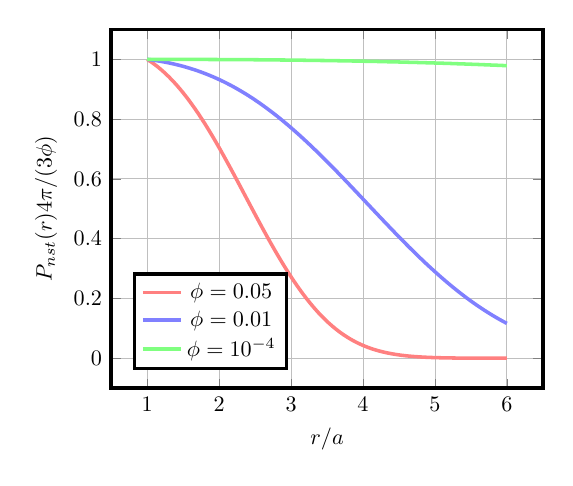
\begin{tikzpicture}[scale=0.8]
    \begin{axis}[
        xlabel={$r/a$},
        ylabel={$P_\text{nst}(r) 4\pi/ (3\phi) $},
        legend style={at={(0.05,0.05)}, anchor=south west},
        grid=major,
        domain=1:6,
        samples=100,
        ultra thick
    ]
    
    % Plot for phi = 0.05
    \addplot[color=red!50,ultra thick]
    { exp(-0.05 * (x^3 - 1))};
    \addlegendentry{$\phi = 0.05$}
    
    % Plot for phi = 0.01
    \addplot[color=blue!50,ultra thick]
    { exp(-0.01 * (x^3 - 1))};
    \addlegendentry{$\phi = 0.01$}
    
    % Plot for phi = 0.001
    \addplot[color=green!50,ultra thick]
    { exp(-0.0001 * (x^3 - 1))};
    \addlegendentry{$\phi = 10^{-4}$}
    
    \end{axis}
\end{tikzpicture}
\hfil
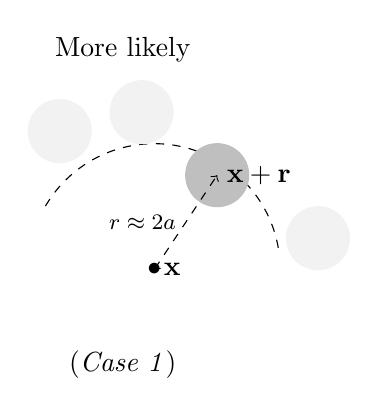
\begin{tikzpicture}[scale=0.8]
  \filldraw[ gray!10!white](+2.6,0.5)circle (0.5);
  \filldraw[ gray!10!white](-1.5,2.2)circle (0.5);
  \draw[dashed](10:2) arc (10:150:2);
  % \filldraw[ gray!50!white](0,0) circle (0.5);
  \filldraw[ gray!50!white](1,1.5)circle (0.5);
  \filldraw[ gray!10!white](-0.2,2.5)circle (0.5);
  \draw(0,0)node{$\bullet$}node[right]{$\textbf{x}$};
  \draw[dashed,<->](0,0)--(1,1.5)node[midway,left]{\footnotesize $r\approx 2 a$}node[right]{$\textbf{x}+\textbf{r}$};
  % \draw[dashed](-0.2,3.5);
  \node[ultra thick] (title) at (-0.5,3.5) {{More likely}};
  \node[ultra thick] (title) at (-0.5,-1.5) {(\textit{Case 1})};
\end{tikzpicture} 
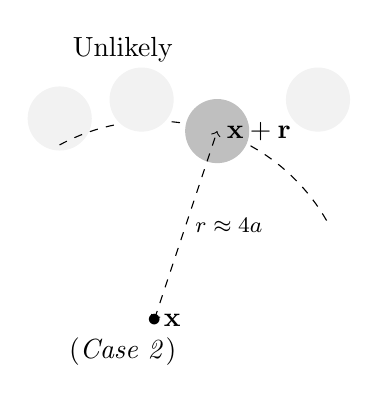
\begin{tikzpicture}[scale=0.8]
  \filldraw[ gray!10!white](+2.6,3.5)circle (0.5);
  \filldraw[ gray!10!white](-1.5,3.2)circle (0.5);
  \draw[dashed](30:3.16) arc (30:120:3.16);
  % \filldraw[ gray!50!white](0,0) circle (0.5);
  \filldraw[ gray!50!white](1,3)circle (0.5);
  \filldraw[ gray!10!white](-0.2,3.5)circle (0.5);
  \draw(0,0)node{$\bullet$}node[right]{$\textbf{x}$};
  \draw[dashed,<->](0,0)--(1,3)node[midway,right]{\footnotesize  $r\approx 4a$}node[right]{$\textbf{x}+\textbf{r}$};
  % \draw[dashed](-0.2,3.5);
  \node[ultra thick] (title) at (-0.5,4.3) {{Unlikely}};
  \node[ultra thick] (title) at (-0.5,-0.5) {(\textit{Case 2})};
\end{tikzpicture} 
\caption{(left) Plot of the normalized nearest neighbor distribution $P_\text{nst}$. 
(right) Sketches explaining the behavior of the nearest neighbor distribution $P_\text{nst}$: 
(\textit{Case 1}) A droplet located at $\textbf{x}+\textbf{r}$ relatively \underline{close} to a point occupied by the continuous phase at \textbf{x}; this situation is likely to happen. 
(\textit{Case 2}) A droplet located at $\textbf{x}+\textbf{r}$ relatively \underline{far} to a point occupied by the continuous phase at \textbf{x}; this situation very unlikely to happen.
Indeed, it implies that no particles are present within the sphere of radius $4a$ centered at $\textbf{x}$ since the nearest neighbor is located at a distance $4a$. 
}
\label{fig:P_nst_f}
\end{figure}
With these assumptions in place, we can compute the \textit{Reynolds stress} using, \ref{eq:relation_ensemble_nst} which reduces to the following formula, 
\begin{equation}
    \avg{\chi_f \textbf{u}_f'\textbf{u}_f'}
    = 
    \frac{3\phi}{4\pi}
    \int_{\mathbb{R}^6}
    \textbf{v}_f^\text{nst}
    \textbf{v}_f^\text{nst}
     e^{-\phi(r^3 -1)}
    d\textbf{r}
    d\textbf{w},
    \label{eq:step_one}
\end{equation}
where it must be understood that $\textbf{v}_f^\text{nst}$ is given by \ref{eq:stokes_sol}. 


Before computing the integration for Stokes flows we would like to apply this formulation to re-compute the \textit{Reynolds stress} of translating bubbles in potential flows. 
Indeed, it can be show that \ref{eq:solution_isolated_at_x} also hols for the \textit{nearest neighbor conditionally averaged} momentum equations in potential flows, thus in that case $\textbf{v}^\text{nst}_f \approx \textbf{u}_f^{1d}$ where we recall that $ \textbf{u}_f^{1d}$ is given by \ref{eq:potential_sol}
Therefore, we carry out the direct integration of \ref{eq:step_one} using \ref{eq:potential_sol} and obtain, 
\begin{equation}
    \avg{\chi_f \textbf{u}_f'\textbf{u}_f'}
    = \Gamma_\text{inc}(-1,\phi)\phi^2 e^\phi \left\{
        \frac{1}{20}[\textbf{u}_{fp}\textbf{u}_{fp}+ \frac{1}{n_p}\pavg{\textbf{u}_\alpha\textbf{u}_\alpha}]
        + 
        \frac{3}{20} (\textbf{u}_{fp}\cdot \textbf{u}_{fp} + 2k_p)\bm\delta
    \right\},
    \label{eq:potential_nst}
\end{equation}
where $\Gamma_\text{inc}$ is the gamma incomplete function. 
According to \ref{eq:potential_nst} our results differ with \ref{eq:van_wingarden_sol} by a factor of $\Gamma_\text{inc}(-1,\phi)\phi^2 e^\phi$. 
Nevertheless, this inconsistency is easily solved noticing that $\Gamma_\text{inc}(-1,\phi)\phi^2 e^\phi \sim \phi + \mathcal{O}(\phi^2)$. 
Thus, we conclude that at the leading order, our methodology seem consistent with the classical conditional average methodology introduced by \citet{batchelor1972sedimentation}. 

Now that we have all the tools in hand, let us carry out the direct integration of \ref{eq:step_one} for the wake of a spherical droplet in stokes flows. 
Indeed, using \ref{eq:solution_isolated_at_x} and \ref{eq:Pnst_explicit} in \ref{eq:step_one} gives, in dimensionless form,  
\begin{equation}
    \avg{\chi_f  \textbf{u}_f'\textbf{u}_f'}^*
    = \phi    
    C_1
    \left\{
        \textbf{u}_{fp}\textbf{u}_{fp}+ \frac{1}{n_p}\pavg{\textbf{u}_\alpha'\textbf{u}_\alpha'}
        -\frac{1}{3} (\textbf{u}_{fp}\cdot \textbf{u}_{fp} + 2k_p)\bm\delta
    \right\},    
    + \phi C_2
    (\textbf{u}_{fp}\cdot \textbf{u}_{fp} + 2k_p)\bm\delta,
    \label{eq:final_closure}
\end{equation}
with,
\begin{align*}
    C_1(\phi,\lambda)
    = \frac{1}{20(1+l)^2}\left[
        \frac{9(2+3\lambda)^2}{4}\Gamma(1/3) \phi^{-1/3}
        - (27+82\lambda +62\lambda^2)
    \right],\\
    C_2(\phi,\lambda)
    = \frac{1}{6(1+l)^2}\left[
        \frac{(2+3\lambda)^2}{4}\Gamma(1/3) \phi^{-1/3}
        - (3+10\lambda +8\lambda^2)
    \right].
\end{align*}
\tb{maybe remove order phi terms}
We have decomposed the \textit{Reynolds stress} tensor into two contribution. 
The first one being, a traceless symmetric tensor, proportional to the functional $C_1$. 
The second contribution is the isotropic part of the \textit{Reynolds stress} tensor, which is proportional to $C_2$. 
This result deserves some comments. 

Firstly, we can notice that, according to the value of $C_1$ and $C_2$, the \textit{pseudo turbulence} or \textit{Reynolds stress} induced by the translation of the droplets is higher for large values of $\lambda$. 
In other words the solid particle induce more wake than a bubble of the same size. 

Secondly, as witnessed by the presence of the term $\phi^{-1/3}$, in $C_1$ and $C_2$, we conclude that the solution obtained here is still consistent with the observation made in \ref{eq:real_error} or in \citet{caflisch1985variance}. 
Indeed, for an isolated droplet, i.e. when we take the limit, $\phi \to 0$, we obtain $\lim_{\phi \to 0} \avg{\chi_f \textbf{u}_f' \textbf{u}_f'} / \phi = \infty$. 
Consequently, in agreement with the previous statements, the normalized \textit{Reynolds stress} is infinite for an isolated droplet, however when considering small but finite value of $\phi$ the \textit{Reynolds stress} remains finite and is given by \ref{eq:final_closure}. 

Finally, as it is not the \textit{Reynolds stress} divided by $\phi$ that matter, but $\avg{\chi_f\textbf{u}_f'\textbf{u}_f'}$ it self, notice that at the leading order in $\phi$ we obtain,  $\avg{\chi_f\textbf{u}_f'\textbf{u}_f'}\sim\phi^{2/3}$. 
Notably, this  trend in $\sim\phi^{2/3}$ is not new and agree with previous studies found in the literature.
Specifically, in \citet{hill2001first} they compute \textit{Reynolds stress} for ordered array of spheres and found $k_f \sim 0.969 \phi^{2/3}$. 
This nearly agree with our \ref{eq:final_closure} with $\lambda =\infty$ as it gives, $k_f  = 1.50$. 



\subsection{The solution at higher order. }

Although we chose to neglect the source term in \ref{eq:momentum_nst_d_stokes} how can we be certain that it was indeed negligible ? 
Even though this term is $\mathcal{O}(\phi)$ higher than the others in $\textbf{v}^\text{nst}$, it does not necessarily imply that it will contribute at $\mathcal{O}(\phi)$ higher than the other terms in $\avg{\rho_f\chi_f \textbf{u}_f'\textbf{u}_f'}$. 
Indeed, in \citet{zhang2021ensemble}, while carrying similar derivation foundout that the terms of $\mathcal{O}(\phi)$ in $\textbf{v}^\text{nst}$ contributed to $\mathcal{O}(\phi^{1/3})$ in their final results. 
In other worlds, this is not as straightforward as in the \textit{single-particles conditional averaged} equations. 

\subsubsection{The velocity fields singularity solution}

Regardless of the right-hand side of \ref{eq:momentum_nst_d_stokes} the boundary condition at the surface of the particle, located at \textbf{y}, will generate the velocity fields\citep{pozrikidis1992boundary}, 
\begin{equation}
    \textbf{v}^\text{nst}_p[\textbf{z},t|\textbf{x},\textbf{w},\textbf{y}]
    = 
    \frac{a}{4}(\textbf{w}- \textbf{u}[\textbf{y},t])\cdot\left[
        \frac{2+3\lambda}{1+\lambda}
        +
        a^2\frac{\lambda}{2(1+\lambda)}\pddz^2 
    \right]\mathcal{G}(\textbf{z},\textbf{y}).
    \label{eq:solution_isolated2}
\end{equation}
Where $\mathcal{G}(\textbf{z},\textbf{y})$ is still the Ossen tensor, or Green function of the stokes equations. 
\tb{En principe la vitesse relative est forme avec la bulk velocity }

Now let us turn our attention to the source term on the right-hand side of \ref{eq:momentum_nst_d_stokes}. 
Following \citet{zhang2021ensemble}, we remark that the contribution to the velocity field, generated by the particle free zone, can be written as a sum of \textit{Stokeslets} of magnitude $\phi\Delta \rho |\textbf{g}|$.
Indeed, the velocity field evaluated at \textbf{z} generated by the point force:  $\phi\Delta \rho \textbf{g}$, located at a generic point $\textbf{x}'$, can be written \citep{pozrikidis1992boundary}, 
\begin{equation}
    \frac{\phi\Delta \rho \textbf{g}}{8\pi \mu_f}\cdot \mathcal{G}(\textbf{z},\textbf{x}')
\end{equation}
Consequently, the velocity fields generated by the particle-free zone, as given in \ref{fig:unst}, can be written \citep{zhang2021ensemble}, 
\begin{equation}
    \textbf{v}_b^\text{nst}[\textbf{z},t|\textbf{y},\textbf{w},\textbf{x}]
    = 
    \frac{\phi\Delta \rho \textbf{g}}{8\pi \mu_f}\cdot 
    \int_{|\textbf{x}'-\textbf{x}|< |\textbf{y}- \textbf{x}|}
    \mathcal{G}(\textbf{z},\textbf{x}')
    d\textbf{x}'
    \label{eq:v_b_sol}
\end{equation}
where we used the subscript $_b$ to denote the particle free zone contribution. 
Due to the linearity of the Stokes equations, the total velocity field is thus the sum of \ref{eq:solution_isolated2} and \ref{eq:v_b_sol}. 
% Likewise, the stress generated by the particle free-zone might be written \citep{pozrikidis1992boundary},
% \begin{equation}
%     \bm\sigma_b^\text{nst}[\textbf{z},t|\textbf{y},\textbf{w},\textbf{x}]
%     = 
%     \frac{\phi\Delta \rho \textbf{g}}{8\pi}\cdot 
%     \int_{|\textbf{x}'-\textbf{x}|< |\textbf{y}- \textbf{x}|}
%     \mathcal{T}(\textbf{z},\textbf{x}')
%     d\textbf{x}'
%     \label{eq:sigma_b_sol}
% \end{equation}
% with, 
% \begin{equation}
%     \mathcal{T}(\textbf{z},\textbf{x}')
%     = - 6\frac{\textbf{rrr}}{r^5}. 
% \end{equation}
% Here, $\textbf{r} = \textbf{z} - \textbf{x}'$. 

Therefore, the total velocity field $\textbf{v}^\text{nst}_f$ at the point $\textbf{x}$, can be obtained using \ref{eq:v_b_sol} and \ref{eq:solution_isolated2} evaluated at the point \textbf{x}, and  \ref{eq:reformulation}, which yields,  
\begin{multline}
    \textbf{v}^\text{nst}_f [\textbf{x},\textbf{w},\textbf{y},t]
    =
    \frac{a}{4}(\textbf{w}- \textbf{u}[\textbf{y},t])\cdot\left[
        \frac{2+3\lambda}{1+\lambda}
        +
        a^2\frac{\lambda}{2(1+\lambda)}\grad^2 
    \right]\mathcal{G}(\textbf{x},\textbf{y})\\
    +
    \phi(\textbf{u}_d - \textbf{u}_f)
    + 
    \frac{\phi\Delta \rho \textbf{g}}{8\pi \mu_f}\cdot 
    \int_{|\textbf{x}'-\textbf{x}|< |\textbf{y}- \textbf{x}|}
    \mathcal{G}(\textbf{x},\textbf{x}')
    d\textbf{x}',
\end{multline}
Carrying out the integral on the second line gives directly,
\begin{equation}
    \int_{|\textbf{x}'-\textbf{x}|< |\textbf{y}- \textbf{x}|}
    \mathcal{G}(\textbf{x},\textbf{x}')
    d\textbf{x}'
    = \frac{8\pi}{3}|\textbf{x}- \textbf{y}|^2\bm\delta
\end{equation}
which finally gives the result, 
\begin{multline}
    \textbf{v}^\text{nst}_f
    =
    \frac{a}{4}(\textbf{w}- \textbf{u}[\textbf{y},t])\cdot\left[
        \frac{2+3\lambda}{1+\lambda}
        +
        a^2\frac{\lambda}{2(1+\lambda)}\grad^2 
    \right]\mathcal{G}(\textbf{x},\textbf{y})
    + 
    \frac{\phi\Delta \rho \textbf{g}}{3\mu_f} |\textbf{x}-\textbf{y}|^2
    +
    \phi(\textbf{u}_d - \textbf{u}_f)
    \label{eq:final_sol_v_nst}
\end{multline}
In this expression we clearly identify $3$ distinct contributions. 
Indeed, the first two terms on the right-hand side of \ref{eq:final_sol_v_nst} correspond to the disturbance field generated by an isolated droplet, which was the only contribution in \ref{eq:solution_isolated_at_x}. 
The third term corresponds to the ``back flow velocity'' as called by \citet{zhang2021ensemble}, it refers to the flow generated by the particle-free zone. 
Finally, the last term ensure that we stay in the right reference frame. 
Notice that in \citet[Appendix A]{zhang2021ensemble} they carried out nearly the same calculation for solid particles.
Apart from that, one can note a small differences between \ref{eq:final_sol_v_nst} with $\lambda = \infty$ and his Equation (B 4), indeed, while we have got$(\textbf{w}- \textbf{u}_f[\textbf{y},t])$ as factor of the first term, he obtained $(\textbf{w}- \textbf{u}_f - \textbf{v}_b^\text{nst})$. 
This is due to the different reference frame used for the velocity fields, indeed, while we have got only one source term at the right-hand side of \ref{eq:momentum_nst_d_stokes} he has a supplementary, constant source term. 
This is the reason for the presence of his $\textbf{v}_b'$ which is not in \ref{eq:final_sol_v_nst}. 
Thus, everything is well consistent, Additionally we generalized and demonstrated his results for droplets. 


For a better physical understanding we present know the dimensionless form of \ref{eq:final_sol_v_nst}. 
The lengths are made dimensionless using the radius of the particle $a$, the velocity vector $\textbf{w} - \textbf{u}$ is made dimensionless the norm $U = |\textbf{w} - \textbf{u}_f|$, 
Indeed, we have the relation, 
\begin{equation*}
    \frac{\textbf{w} - \textbf{u}}{|\textbf{w} - \textbf{u}_f|}
    = \textbf{e} + \phi \textbf{e}
\end{equation*}
where we introduced the unit vector: $\textbf{e} = \textbf{w} - \textbf{u}_f/U$. 
Likewise, the gravity acceleration vector is made dimensionless using its norm, such that the unit vector in the direction of the acceleration of gravity is given by $\textbf{k} = \textbf{g} / g$, with $g = |\textbf{g}|$. 
Dividing \ref{eq:final_sol_v_nst} by $U$ and using these definitions yields directly the dimensionless expression for the disturbance velocity field, 
\begin{equation}
    \frac{\textbf{v}^\text{nst}_f}{U}
    =
    \frac{1}{4}(\textbf{e}+ \phi \textbf{e})\cdot\left[
        \frac{2+3\lambda}{1+\lambda}
        +
        \frac{\lambda}{2(1+\lambda)}\grad^2 
    \right]\mathcal{G}(\textbf{x},\textbf{y})
    + \phi A |\textbf{x}-\textbf{y}|^2 \textbf{k}
    +\phi \textbf{e}
    \label{eq:v_nst_solution_adim}
\end{equation}
where we kept the same notation for all the distances, they are assumed implicitly dimensionless. 
At the leading order, notice that the terms proportional to $\phi \textbf{e}$ in \ref{eq:v_nst_solution_adim} are negligible, however we keep them for the purpose of generality. 
Additionally, we introduced the dimensionless number, 
\begin{equation}
    A = \frac{Ar}{12 Re}=\frac{\Delta \rho g (2a)^2}{12 \mu_f U}
    \label{eq:A_general}
\end{equation}
where we recall that $Ar$ is the \textit{Galileo} number and $Re$ the \textit{Reynolds} number, defined as,  
\begin{align*}
    Re= \frac{\rho_f U 2a}{\mu_f},
    &&
    Ar = \frac{\rho_f \Delta\rho g (2a)^3}{\mu_f^2},
\end{align*}
respectively. 
Upon considering specific scenarios, such as a steady state rising droplet due to the acceleration of gravity, one is able to relate $Ge$ and $Re$ and give explicit closure instead of $A$. 
As mentionned in \citet{zhang2021ensemble} this approaches can be generalized to other body forces fields, such as electromagnetic forces, in order to obtain the influence of the latter on the resulting velocity field.

\subsubsection{The pseudo turbulent tensor closure}

From \ref{eq:sol_dimenisonless_results} we may already compute the integral in \ref{eq:step_one}. 
However, as $\textbf{e}$ and $\textbf{k}$ in \ref{eq:sol_dimenisonless_results}  are not necessarily collinear vectors the functional form of the resulting stress tensor is not trivial. 
% Thus, in the first place we clarify the expected functional form of $\avg{\rho_f \textbf{u}_f'\textbf{u}_f'}$. 
Indeed, since $\textbf{v}_f^\text{nst}\sim \textbf{e}$ or $\textbf{g}$, the final results must be a tensor built from sum of product of these two vectors.  
Additionally, since $\avg{\rho_f \textbf{u}_f'\textbf{u}_f'}$ is a symmetric tensor, the result must be a symmetric tensor as well. 
Since, the only second order symmetric tensors that can be constructed from the  two arbitrary vectors: $\textbf{e}$ and $\textbf{k}$ are, 
\begin{align*}
    \textbf{ee}
    && (\textbf{e}\cdot \textbf{e})\bm\delta, 
    && \textbf{kk},
    && (\textbf{k}\cdot \textbf{k})\bm\delta,
    && \textbf{ke}+\textbf{ek},
    && (\textbf{k}\cdot \textbf{e})\bm\delta, 
\end{align*}
we deduce that the volume integral of \ref{eq:step_one}, have the form, 
\begin{align}
    \frac{1}{U^2}
    \frac{3\phi}{4\pi}\int_{\mathbb{R}^3}
    \textbf{v}_f^\text{nst}
    \textbf{v}_f^\text{nst}
     e^{-\phi(r^3 -1)}
    d\textbf{r}
    &= C^{(1)}_e \left[
        \textbf{ee}
         - \frac{1}{3}(\textbf{e}\cdot \textbf{e})\bm\delta
    \right]
    + C^{(2)}_e 
    (\textbf{e}\cdot \textbf{e})\bm\delta \nonumber \\
    &+ C^{(1)}_k \left[
        \textbf{kk}
         - \frac{1}{3}(\textbf{k}\cdot \textbf{k})\bm\delta
    \right]
    + C^{(2)}_k 
    (\textbf{k}\cdot \textbf{k})\bm\delta \nonumber \\
    &+ C^{(1)}_{ek} \frac{1}{2}\left[
        (\textbf{ek}  + \textbf{ke})
         - \frac{2}{3}(\textbf{k}\cdot \textbf{e})\bm\delta
    \right]
    + C^{(2)}_{ek} 
    (\textbf{e}\cdot \textbf{k})\bm\delta 
    \label{eq:functional_form}
\end{align}
where the first term of each line correspond to symmetric traceless tensors, and the second term of each line to the corresponding isotropic contribution. 
Then, the first two constant, $C^{(1)}_e$ and $C^{(2)}_e$ can be obtained setting $\textbf{g}= 0$ in \ref{eq:sol_dimenisonless_results} and performing the integration. 
Likewise, $C^{(1)}_k$ and $C^{(2)}_k$ can be obtained setting $\textbf{e}=0$ in \ref{eq:sol_dimenisonless_results}. 
The constants, $C^{(1)}_{ek}$ and $C^{(2)}_{ek}$ can be obtained setting $\textbf{g} = 0$ in of the $\textbf{v}_f^\text{nst}$ on the left-hand side of \ref{eq:functional_form} and $\textbf{e}=0$ in the other $\textbf{v}_f^\text{nst}$. 
Thus, we directly, obtain at the leading order, 
\begin{align}
    C_e^{(1)} =
    % \frac{9(2+3\lambda)^2 \Gamma(\frac{1}{3})}{80(\lambda+1)^2}\phi^{2/3}
    \frac{27}{10}
    C_e^{(2)}
    % + \mathcal{O}(\phi)
    &&  C_e^{(2)} =
    \frac{(2+3\lambda)^2 \Gamma(\frac{1}{3})}{24(\lambda+1)^2}\phi^{2/3}
    + \mathcal{O}(\phi)
    \\
    C_k^{(1)} =
    % A^2 \Gamma\left(7/3\right)\phi^{2/3}
    3
    C_k^{(2)}
    % + \mathcal{O}(\phi^{5/3})
    && C_k^{(2)} =
    A^2 \frac{\Gamma(\frac{7}{3})}{3}\phi^{2/3}
    + \mathcal{O}(\phi^{5/3})
    \\
    C_{eg}^{(1)} =
    3
    C_{eg}^{(2)}
    % A\frac{2 (2+3\lambda) \Gamma(\frac{4}{3})}{3 (\lambda+1)}\phi^{2/3}
    % + \mathcal{O}(\phi^{4/3})
    && C_{eg}^{(2)} =
    A\frac{2 (2+3\lambda) \Gamma(\frac{4}{3})}{9(\lambda+1)}\phi^{2/3}
    + \mathcal{O}(\phi^{4/3})
    \label{eq:constants}
\end{align}
As can be seen, the leading order contribution from the back flow velocity generated due to the acceleration of gravity is $\sim \phi^{2/3}$. 
It is therefore non-negligible in this general framework. 
\tb{include the orer phi terms .  ?  ? ? }


Following \ref{eq:step_one} to obtain the \textit{Reynolds stress} tensor we now integrate  \ref{eq:functional_form} over the $\textbf{w}$, which yield the final form of our \textit{Pseudo turbulent} tensor model, namely, 
\begin{align}
    \frac{\avg{\chi_f \textbf{u}_f'\textbf{u}_f'}}{U^2}
    &= 
    C^{(1)}_e \left[
        \textbf{e}_p\textbf{e}_p
        + \frac{\pavg{\textbf{u}_\alpha'\textbf{u}_\alpha'}}{n_p U^2}
         - \frac{1}{3}(\textbf{e}_p\cdot \textbf{e}_p+2k_p/U^2)\bm\delta
    \right]
    + C^{(2)}_e 
    (\textbf{e}_p\cdot \textbf{e}_p+2k_p/U^2)\bm\delta \nonumber \\
    &+ C^{(1)}_k  \left[
        \textbf{kk}
         - \frac{1}{3}(\textbf{k}\cdot \textbf{k})\bm\delta
    \right]
    +C^{(2)}_k 
    (\textbf{k}\cdot \textbf{k})\bm\delta \nonumber \\
    &+ C^{(1)}_{ek} \left[
        \frac{1}{2}
        (\textbf{e}_p\textbf{k}  + \textbf{k} \textbf{e}_p)
         - \frac{1}{3}(\textbf{k}\cdot \textbf{e}_p)\bm\delta
    \right]
    + C^{(2)}_{ek}
    (\textbf{e}_p\cdot \textbf{k})\bm\delta 
    \label{eq:functional_form_avg}
\end{align}
In this expression $\textbf{e}_p = \int \textbf{e} d\textbf{w} $ represents the mean direction of the mean relative phase velocity $\textbf{u}_{pf}$ such that $\textbf{u}_{pf} = U \textbf{e}_p$, in opposition to $\textbf{e}$ which represented the direction of a single particle relative velocity. 



In summary, the only additional terms appearing due to the integration over the velocity phase space is the addition of the particle fluctuation contribution to the \textit{Reynolds stress}. 
However, it is likely that $k_p/U^2 \sim \phi$ at least, therefore at $\mathcal{O}(\phi)$ this term might be safely neglected. 
However, for purpose of generality we keep these terms. 



\subsubsection{Steady-state rising droplet}

Let us now study the case where $\textbf{k} = - \textbf{e} = \textbf{e}_z$, meaning that the droplet rises in the opposite direction of gravity which is aligned with the vertical direction denoted by $\textbf{e}_z$.  
At $\mathcal{O}(\phi)$ and in Stokes flow regime, the drag applied on an isolated spherical droplet is given by Hadamard-Ribczynski formula, thus at steady-state the rising velocity of a droplet is given by, 
\begin{equation}
    U = \Delta \rho \frac{g (2a)^2}{6 \mu_f }\left(\frac{1+\lambda}{2+3\lambda}\right).
    \label{eq:U_isolated}
\end{equation}
% \begin{equation}
%     2a \pi \mu_f \left(\frac{3\lambda +2}{\lambda +1}\right) 
%     U
%     = 
%     \frac{4}{3}\pi a^3 
%     \Delta \rho
%     g,
% \end{equation}
We deduce from this relation that in this specific situation, i.e. when the direction of the relative velocity \textbf{e} is aligned with the gravity acceleration direction, we have, 
\begin{equation}
    A = \frac{1}{2}\left(\frac{3\lambda +2}{\lambda +1}\right). 
    \label{eq:closure_A}
\end{equation}
Injecting this expression into \ref{eq:v_nst_solution_adim} gives us an explicit expression of the velocity field $\textbf{v}^\text{nst}_f$. 

To give a better idea of the meaning of $\textbf{v}_f^\text{nst}$, we display 
in \ref{vnst_vertical} the streamlines generated by the field $\textbf{v}_f^\text{nst}(\textbf{r})$ in the cross-section, given by the plane formed by the vectors $(\textbf{e}_x,\textbf{e}_z)$. 
\begin{figure}[h!]
    \centering
    \includegraphics[height = 0.33\textwidth]{image/Vnst_l_10_0.pdf}
    \includegraphics[height = 0.33\textwidth]{image/Vnst_l_10_1.pdf}
    \includegraphics[height = 0.33\textwidth]{image/Vnst_l_10_5.pdf}
    % \includegraphics[height = 0.33\textwidth]{image/Vnst_l_10_10.pdf}
    \caption{Streamlines of the disturbance velocity field $\textbf{v}^\text{nst}(\textbf{r}_f)$ \eqref{eq:v_nst_solution_adim}  in the cross-section given by the plane $(\textbf{e}_x,\textbf{e}_z)$, for multiples volume fraction $\phi = 0, 0.01$ and $0.05$ at $\lambda = 10$.  
    The color map indicates the magnitude of the velocity, from black which corresponds to a velocity magnitude of 0, to the color at the interface which corresponds to 1.
    In this situation $\textbf{e} = \textbf{e}_z$ and $\textbf{k} = -\textbf{e}_z$}
    \label{fig:vnst_vertical}
\end{figure}
We can observe on \ref{fig:vnst_vertical} (left) that $\textbf{v}^\text{nst}_f(\phi =0)$ corresponds to the disturbance field of an isolated particle in Stokes flow. 
This is easily understandable considering that the last two terms on the right-hand side of \ref{eq:v_nst_solution_adim} cancel for $\phi=0$, thus leading to \ref{eq:solution_isolated} which is the solution for isolated particle. 
At finite volume fraction, $\phi =0.01$, we  observe in \ref{fig:vnst_vertical} (middle), that a downstream velocity start to appear at large distance from the particle center.  
As discussed previously, this ``back flow velocity'' is given by the term $\phi A |\textbf{x}- \textbf{y}|^2 \textbf{k}$ in \ref{eq:solution_isolated}.
The particle is thus surrounded by a spherical shell within which the disturbance field has a positive vertical velocity, and outside which the velocity is negative.
In the following discussion we call this spherical shell the \textit{confinement zone}.   
For higher volume fractions $\phi = 0.05$, the backflow velocity is even stronger leading to a smaller confinement zone around the particle. 

Let us discuss the form of \ref{eq:functional_form_avg} in the specific case displayed in \ref{fig:vnst_vertical}, i.e. spherical droplets rising in stokes flow. 
Since $\textbf{e}_p = - \textbf{k}$ we have $\textbf{e}_p\textbf{k} = - \textbf{kk}$. 
Additionally, one can use \ref{eq:closure_A} into the expression for $C_k^{(1)}$ and $C_{ek}^{(1)}$. 
In this specific case, by carrying out the calculation, we obtain, 
\begin{equation}
    C_k^{(1)} \textbf{kk} + C_{ek}^{(1)} \textbf{ke}_p
    = 0. 
    \label{eq:cancelation1}
\end{equation}
Applying the same reasoning, one can also deduce that, 
\begin{equation}
    C_k^{(2)} \textbf{k}\cdot \textbf{k} + C_{ek}^{(2)} \textbf{k}\cdot \textbf{e}_p
    = 0. 
    \label{eq:cancelation2}
\end{equation}
Consequently, we must deduce that the contribution from the gravity acceleration to the \textit{Reynolds stress} tensor, remains negligible in this simplified situation. 
This, might seem surprising considering the seemingly non-negligible action of the gravity on the velocity field displayed \ref{eq:vnst_vertical}. 
However, we must understand from this fact, that the velocity variance generated by the back flow velocity, also induce a decrease of the velocity variance generated by the particle motion compared to the isolated case.
In other word, the back flow velocity generate at the boundaries of the confinement zone a low velocity variance, which is exactly balanced by the velocity variance generated by the back flow at the exterior of the confinement zone.    
Notice that this explanation is only true when, $\textbf{k} = - \textbf{e}_p$. 
Thus, we may examine now situations were the velocity of the dispersed phase is not in the opposite direction of gravity. 



\subsubsection{Horizontal motions}

We now consider the case were $\textbf{e}_p = \textbf{e}_x$, and $\textbf{k} = - \textbf{e}_z$, where $\textbf{e}_z$ is still the vertical unit vector and $\textbf{e}_x$ the Horizontal unit vector. 
Of course in the steady-state isolated regime $\textbf{e}_p$, could not be otherwise than vertical. 
However, in a more general case, consider an Euler-Euler framework for example, $\textbf{e}_p$ have absolutely no reason to be in the vertical direction, due to boundaries or transient effects. 
In this case $A$ is given by \ref{eq:A_general} and requires the norm of the relative velocity $U$ which is supposed known in the Euler-Euler simulation. 

\begin{figure}[h!]
    \centering
    \includegraphics[height = 0.33\textwidth]{image/Vnst_H_l_10_0.pdf}
    \includegraphics[height = 0.33\textwidth]{image/Vnst_H_l_10_1.pdf}
    \includegraphics[height = 0.33\textwidth]{image/Vnst_H_l_10_5.pdf}
    % \includegraphics[height = 0.33\textwidth]{image/Vnst_l_10_10.pdf}
    \caption{Streamlines of the disturbance velocity field $\textbf{v}^\text{nst}(\textbf{r}_f)$  \eqref{eq:v_nst_solution_adim} in the cross-section given by the plane $(\textbf{e}_x,\textbf{e}_z)$, for multiples volume fraction $\phi = 0, 0.01$ and $0.05$ at $\lambda = 10$.  
    The color map indicates the magnitude of the velocity, from black which corresponds to a velocity magnitude of 0, to the color at the interface which corresponds to 1.
    In this situation $\textbf{e} = \textbf{e}_x$ and $\textbf{k} = -\textbf{e}_z$.
    The constant $A$ have been arbitrarily set to $1$. }
    \label{fig:vnst_horizontal}
\end{figure}
In \ref{fig:vnst_horizontal} we display the streamlines generated by the velocity field $\textbf{v}_f^\text{nst}$ in this situation. 
As before, we remark that at $\phi = 0$, $\textbf{v}_f^\text{nst}$ corresponds to the disturbance velocity field of an isolated droplet translating Horizontally in Stokes flow. 
At $\phi = 0.01$, see \ref{fig:vnst_horizontal} (middle), the effect of gravity induce a downstream flow, which is, this time not in the opposite direction of the disturbance velocity of the drop, resulting into a global down-right flow. 
At higher volume fraction this down stream flow is stronger, and the confinement zone around the particle smaller. 
In summary, we observe the same phenomenon as in the previous situation reported on \ref{fig:vnst_vertical}, except that the droplet disturbance field is not in the opposite direction of the back flow velocity, but normal to it.

This difference has a significant impact on the \textit{Reynolds stress} closure, as the relation \ref{eq:cancelation1} and \ref{eq:cancelation2} are not true anymore. 
Indeed, in this case the functional form of the \textit{Reynolds stress} is given by, 
\begin{equation}
    \frac{\avg{\chi_f \textbf{u}_f'\textbf{u}_f'}}{U^2}
    = 
    C^{(1)}_e 
    \textbf{e}_x\textbf{e}_x
    % + \frac{\pavg{\textbf{u}_\alpha'\textbf{u}_\alpha'}}{n_p U^2}
    +C^{(1)}_k    
    \textbf{e}_z\textbf{e}_z
    - C^{(1)}_{ek} 
        \frac{1}{2}
        (\textbf{e}_x\textbf{e}_z+ \textbf{e}_z \textbf{e}_x)
    + [C^{(2)}_e + C^{(2)}_k - (C^{(1)}_k + C^{(1)}_e )/3 ]  \bm\delta. 
\end{equation}
Thus, the contribution from the wake of the particles is still present and given by $C_e^{(1)}$ and $C_e^{(2)}$. 
Regarding the buoyancy forces, it provides additional contributions that are on the vertical direction. 
Finally, the cross term $\textbf{e}_p \textbf{k}$ provides off-diagonal terms. 
The isotropic part of this tensor is the sum of the aforementioned contributions. 

\subsection{Discussion}

In this section we have considered the translating motion of a spherical droplet in stokes flow. 
In this regime we have shown that the ambient body force field $\textbf{g}$ plays a non-negligible role on the \textit{Nearest Neighbor Conditional Averaged} disturbance fields. 
Consequently, the \textit{Reynolds stress} closure obtained is a function of $\textbf{u}_{fp}$ the relative phase velocity and the direction of $\textbf{g}$ which is considered vertical. 

To extend this model one might consider a more general ambient field, not only a uniform velocity field as demonstrated now. 
This is the purpose of the last section of this chapter. 
However, as this theoretical approaches is for the most of it new, we focus on the section on the numerical validation of this model. 

% \section{Numerical experiments. }

In this section, we compare the theoretical results, to the numerical results obtained with \texttt{Basilisk} introduced in \ref{chap:DNS}. 
We recall that we are working with a set of simulations covering the parameter ranges displayed in \ref{tab:simulations_recall}. 
\begin{table}[h!]
    \centering
    \caption{Dimensionless parameter ranges investigated in this work.}
    \begin{tabular}{|ccccccc|ccc|}
        \hline
        \multicolumn{7}{|c}{Primary parameters} & \multicolumn{3}{||c|}{Secondary parameters}\\ \hline
        \multicolumn{1}{|c|}{$Ga$}                               & \multicolumn{1}{c|}{$Bo$}                   & \multicolumn{1}{c|}{$\phi$} & \multicolumn{1}{c|}{$\lambda$}                    & \multicolumn{1}{c|}{$\zeta$}                & \multicolumn{1}{c|}{$N_b$} & $t^*_\text{end}$ & \multicolumn{1}{||c|}{$\mathcal{L}/d$} & \multicolumn{1}{c|}{$Re$}  & $We$   \\ \hline
        \multicolumn{1}{|c|}{\multirow{4}{*}{$5\rightarrow 80$}} & \multicolumn{1}{c|}{\multirow{4}{*}{$0.5$}} & \multicolumn{1}{c|}{$1\%$}  & \multicolumn{1}{c|}{\multirow{4}{*}{$10$ \& $1$}} & \multicolumn{1}{c|}{\multirow{4}{*}{$0.9$}} & \multicolumn{1}{c|}{$160$} & $400$           & \multicolumn{1}{||c|}{$20$}            & \multicolumn{1}{c|}{$1.1\to 110$} & {$0.03\to 0.95$} \\ 
        \multicolumn{1}{|c|}{}                                   & \multicolumn{1}{c|}{}                       & \multicolumn{1}{c|}{$5\%$}  & \multicolumn{1}{c|}{}                             & \multicolumn{1}{c|}{}                       & \multicolumn{1}{c|}{$800$} & $400$           & \multicolumn{1}{||c|}{$20$}            & \multicolumn{1}{c|}{$0.8\to 92$} &  {$0.02\to 0.67$}\\ 
        \multicolumn{1}{|c|}{}                                   & \multicolumn{1}{c|}{}                       & \multicolumn{1}{c|}{$10\%$} & \multicolumn{1}{c|}{}                             & \multicolumn{1}{c|}{}                       & \multicolumn{1}{c|}{$200$} & $1000$           & \multicolumn{1}{||c|}{$10$}            & \multicolumn{1}{c|}{$0.64\to 77$}&  {$0.01\to 0.47$}\\ 
        \multicolumn{1}{|c|}{}                                   & \multicolumn{1}{c|}{}                       & \multicolumn{1}{c|}{$20\%$} & \multicolumn{1}{c|}{}                             & \multicolumn{1}{c|}{}                       & \multicolumn{1}{c|}{$400$} & $1000$           & \multicolumn{1}{||c|}{$10$}            & \multicolumn{1}{c|}{$0.43\to 62$}&  {$9\cdot 10^{-3}\to 0.31$}\\ \hline
        \end{tabular}
    \label{tab:simulations_recall}
\end{table}
In the first step, we will make use of the simulation results at $Ga = 5$ which is considered to be comparable to the Stokes regime used for the theory. 
However, note that at $Ga = 5$, $Re \approx 1$ consequently inertial effects are already present. 
Nevertheless, due to numerical constraints lower \textit{Reynolds} numbers could not be reached. 

The two main results that we are seeking to validate are, the disturbance fields expression \eqref{eq:v_nst_solution_adim} and the \textit{Reynolds} stress closure tensor, \eqref{eq:functional_form_avg}. 
Consequently, in the first part of this section, we focus on the comparison of $\textbf{v}_f^\text{nst}$ obtained with the DNS to the solution given by \ref{eq:v_nst_solution_adim}.
Then, we compare the numerical value of $\avg{\chi_f \textbf{u}_f'\textbf{u}_f'}$ with the prediction of \ref{eq:functional_form_avg}. 
Finally, our goal will be to extend \ref{eq:functional_form_avg} to non-negligible inertial effect and volume fraction effects, i.e. to higher $Re$ and $\phi$. 

\subsection{Nearest neighbors conditionally averaged disturbance velocity}

To reconstruct $\textbf{v}_f^\text{nst}$ with the DNS we must discretize \ref{eq:def_f_nst}. 
We proceed as follows: 
(1) We consider all simulations time steps and locations in the mesh as an independent configuration $\FF$.
This assumption holds since the system is homogeneous and statistically steady in time.  
Thus, we consider that the field $\textbf{u}_f^0[\textbf{x},\FF,t]$ is given by the field $\textbf{u}[c,t]$, where $c$ is the label of a given cell in the mesh and $t$ the time step of the simulation. 
Here, it must be understood that $\FF$ corresponds to all different combinations of $c$ and $t$. 
(2) Finally, we discretize the distance vector $\textbf{r}$ from a point in the mesh to the center of mass of the nearest neighbor, in $n^{th}$ intervals, with the location of the center of the $k^{th}$ interval denoted by $\textbf{r}_k$, where $\textbf{r}_k = 1,\ldots,n$. 
Under these hypotheses, the \textit{nearest neighbors conditionally averaged} velocity fields, $\textbf{u}_f^\text{nst}$, can be obtained numerically as, 
\begin{equation}
    \textbf{u}_f^\text{nst}(\textbf{r}_k)
    = 
    \frac{1}{E_k}
    \sum_{\FF_k}^{E_k}
    \sum_i^N
    \textbf{u}[c,t] h_i[c,t],
    \label{eq:vnst_DNS}
\end{equation}
where $E_k$ corresponds to the total number of events and $N$ to the total number of particles in the flow.
$h_i[c,t]$ corresponds to the function $h_i[\textbf{x},t,\FF]$  (see \ref{eq:h_i_def}), evaluated at time step $t$ and at the center of cell $c$. 
Thus, $h_i[c,t] = 1$ when the $i^{th}$ droplet is the nearest neighbor to the location of the cell center $c$. 
$h_i[c,t]$ is a function of the droplet's center of mass positions, which are obtained using the same approach as in the previous chapters.
Then, to recover $\textbf{v}_f^\text{nst}/U$ from $\textbf{u}_f^\text{nst}$, we simply measure the mean relative phase velocity $U$ within the DNS, and use the formula: $\textbf{v}_f^\text{nst} /  U = \textbf{u}_f^\text{nst} / U -1 $. 



Because our DNS represents rising droplets in the direction of buoyancy, our results are to be compared with the theoretical prediction displayed on \ref{fig:vnst_vertical}. 
Thus, in \ref{fig:vnst_DNS} we display the reconstructed velocity fields based on the DNS, according to \ref{eq:vnst_DNS}, against the theoretical prediction given by \ref{eq:v_nst_solution_adim}. 
\begin{figure}
    \centering
    \includegraphics[width = 0.32\textwidth]{image/HOMOGENEOUS_final/Stream/Stream_PHI_1_Ga_5_l_10.pdf}
    \includegraphics[width = 0.32\textwidth]{image/HOMOGENEOUS_final/Stream/Stream_PHI_5_Ga_5_l_10.pdf}
    \includegraphics[width = 0.32\textwidth]{image/HOMOGENEOUS_final/Stream/Stream_PHI_5_Ga_80_l_10.pdf}
    \caption{Streamlines of the disturbance velocity field $\textbf{v}^\text{nst}$, in the cross-section given by the plane $(\textbf{e}_x,\textbf{e}_z)$, for two volume fractions $\phi = 0.01$ (left) and $\phi = 0.05$ (middle) at $\lambda = 10$ and $Ga = 5$.
    (right) plot of the inertial case $Ga = 80$. 
    On the left side of the panel ($x/a < 0$), we have re-plotted the theoretical solution provided by \ref{eq:v_nst_solution_adim}.   
    On the right side of the panel ($x/a > 0$), we have reconstructed the streamlines obtained with the DNS, using \ref{eq:vnst_DNS}. 
    The color map indicates the magnitude of the velocity, from black which corresponds to a velocity magnitude of 0, to the color at the interface of the droplet which corresponds to a magnitude of 1.}
    \label{fig:vnst_DNS}
\end{figure}
As seen on \ref{fig:vnst_DNS}:  %the common points that shear the velocity fields from the DNS to the theoretical prediction are the following: 
(1) both velocity fields exhibit approximately the same wake close to the interface of the droplet. 
That is the wake of an isolated rising vertical droplet. 
(2) For a distance large enough from the droplet center we see the downstream flow appears.
(3) The recirculation region, delimited by the null radial velocity (i.e. for the points $\textbf{r}$ following $\textbf{v}^\text{nst}\cdot \textbf{r} = 0$ with $|\textbf{r}|>a$), follows the same trends as the theoretical prediction, i.e. the radius is smaller for higher $\phi$. 
Additionally, the radii of the recirculation region have approximately the same size for both cases where $Ga = 5$. 

Regarding the differences, we can note that for the case $\phi = 0.01$, displayed on \ref{fig:vnst_DNS} (left) the wake of the particle is slightly asymmetric, while the theoretical solution is purely symmetric. 
The fore-aft symmetry of the wake of a particle as displayed in \ref{fig:vnst_vertical} is typically due to the absence of inertial effect. 
Thus, the non-fore-aft symmetry observed on the plot, \ref{fig:vnst_DNS} (left), is due to the non-negligible inertial effect present for this case. 
Indeed, as reported in \ref{tab:simulations_recall} the \textit{Reynolds} number for this case is $Re \approx 1$, implying that the inertial effects cannot be neglected. 
In opposition at $\phi = 0.05$, the numerical results exhibit a nearly fore-aft symmetric wake. 
This is consistent with the previous remark since for this case $Re < 1$. 

To extend our understanding we have also displayed on \ref{eq:vnst_DNS} (right) a high inertial case, with  $Ga = 80$. 
In this case, we see that the wake exhibits fore-aft asymmetry, which confirms that this trend comes with inertial effects. 
Additionally, we can note that the top boundary of the recirculation region is approximately at the same location as the theoretical prediction. 
However, the downstream boundary is different from the one predicted by the theoretical prediction, again that is because the fore-aft symmetry of the flow is broken.  
The symmetry of a distribution can be quantified by the ``skewness'' of the distribution. 
In the case of the continuous phase velocity distribution it is the triple velocity correlation $\avg{\chi_fk_f  \textbf{u}_f'}$ appearing in the pseudo turbulent energy equation \eqref{eq:dt_hybrid_k1}, that quantify the fore-aft symmetry.
As demonstrated, in Stokes regime $\avg{\chi_fk_f  \textbf{u}_f'} = 0$ due to the fore-after symmetry of the disturbance fields of spherical particles.  
Hence, the effect of inertia, which generates a fore-aft asymmetry in the particle's wake, will not necessarily impact the velocity variance but rather the skewness of the velocity distribution. 


To conclude, we can state that \ref{eq:v_nst_solution_adim} is well representative of the velocity field reconstructed with the DNS. 
Therefore, we can be confident regarding the accuracy of our \textit{Reynolds} stress closure at least for low \textit{Galileo} numbers. 




\subsection{Vertical velocity variance}

As discussed in the previous section, in the situation reproduced by the DNS, the velocity variance is given by \ref{eq:functional_form_avg} without the contribution of the buoyancy term (see \eqref{eq:cancelation1} and \ref{eq:cancelation2}). 
Additionally, for instance, we assert that the particle vertical velocity variance $\pavg{\textbf{u}_\alpha'\textbf{u}_\alpha'}_{zz}$ is negligible  at  $Ga =5$. 
In the next subsections, we show that this assumption is indeed confirmed by the DNS results. 
However, for the horizontal velocity variance, we will observe that it is not necessarily a valid assumption. 
Under these conditions, the vertical component of the velocity variance given by \ref{eq:functional_form_avg} is expressed as, 
\begin{equation}
    \frac{\avg{\chi_f \textbf{u}_f'\textbf{u}_f'}_{zz}}{\phi_f U^2}
    = \phi^{2/3} \left(
        \frac{2}{3}C_e^{(1)}+ C_e^{(2)}
    \right)
    = 
    \phi^{2/3}\Gamma\left(\frac{1}{3}\right) \frac{7}{60}\frac{(2+3\lambda)^2 }{(\lambda+1)^2}
    % \left(e^{-Re} - 1 \right)/2
    + \mathcal{O}(\phi), 
    % . 
    \label{eq:theoritical_simplified}
\end{equation}
where we recall that $\Gamma(1/3) \approx 2.67894$. 




\subsubsection{Comparison with the DNS results}

In \ref{fig:uuyy} we compare the vertical velocity variance given by \ref{eq:theoritical_simplified} to the numerical results.
At low volume fraction and for all $\lambda$ good agreements are obtained. 
Interestingly for all $\lambda$, \ref{eq:theoritical_simplified} seems to provide a good estimation for the Reynolds stress even at high volume fraction $\phi$, especially viscous droplets ($\lambda = 10$). 
Since no particle interaction terms of any kind are considered in the theory, this good agreement is probably fortuitous.
\begin{figure}
    \centering
    % \includegraphics[height = 0.25\textwidth]{image/HOMOGENEOUS_final/CA/cartellier.pdf}
    \includegraphics[height = 0.25\textwidth]{image/HOMOGENEOUS_final/CA/UUyy_Ga_5.pdf}
    \caption{Dimensionless value of the vertical velocity variance  as a function of the volume fraction $\phi$ for various $\lambda$ in the low inertial regime ($Ga = 5$). 
    % (left) Experimental  results  of \citet{cartellier2009induced} compared to \ref{eq:theoritical_simplified} with $\lambda = 0$ (dash dotted line) original scaling of \citet{cartellier2009induced}. 
    Comparison of the ``Present theory'' \eqref{eq:theoritical_simplified} against the velocity variance obtained with DNS results according to \eqref{eq:def_uuf_num}. 
    }
    \label{fig:uuyy}
\end{figure}
The red dashed line in \ref{fig:uuyy} (right) represents the potential flow solution of \citet{biesheuvel1984two} given by \ref{eq:van_wingarden_sol}. 
This model underpredicts the magnitude of the vertical pseudo-turbulence.
We deduce that the velocity variance produced by droplets in Stokes flow is much larger than the one in potential regime. 


\subsubsection{Comparison with the literature}

In \ref{fig:uuyy2}  we compare \ref{eq:theoritical_simplified} with $\lambda = 0$ to the  experimental measurements of \citet{cartellier2009induced}. 
We observe reasonable agreements from $\phi = 10^{-3}$ to moderate volume fraction ($\phi \approx 0.03$). 
In the low volume fraction regime \citet{cartellier2009induced} found that $\avg{\chi_f\textbf{u}_f'\textbf{u}_f'} / U^2 \sim \phi^{0.7 \pm 0.03}$,  while \ref{eq:theoritical_simplified} with $\lambda = 0$ predicts, $\avg{\chi_f\textbf{u}_f'\textbf{u}_f'} / U^2 \sim 1.25017 \cdot \phi^{2/3} $. 
Thus, our results overestimate \citet{cartellier2009induced} best fits by $25\%$. 
This may be explained by the non-negligible inertial effects present in \citet{cartellier2009induced} experiments.
Indeed, the bubble Reynolds number measured in \citet{cartellier2009induced} is about $10$, while our theory is limited to Stokes flow. 
\begin{figure}
    \centering
    \includegraphics[height = 0.25\textwidth]{image/HOMOGENEOUS_final/CA/cartellier.pdf}
    \caption{Dimensionless value of the vertical velocity variance  as a function of the volume fraction $\phi$ for various $\lambda$ in the low inertial regime ($Ga = 5$). 
    (dots) Experimental  results  of \citet{cartellier2009induced}.
    (dashed line) Theoretical formula \ref{eq:theoritical_simplified} with $\lambda = 0$.
    % (dash dotted line) \citet{cartellier2009induced}'s original scaling. 
    }
    \label{fig:uuyy2}
\end{figure}

It is reasonable to assume that the slight disparities observed between these results and the theory are due to the inertial effects or a non-negligible volume fraction effect. 
Considering the good agreements obtained with both, the numerical results and \citet{cartellier2009induced} experiments, we can state that \ref{eq:theoritical_simplified} predicts with a reasonable accuracy the droplets induced turbulence in low Reynolds and dilute suspensions.  

\subsection{Horizontal velocity variance}

We turn now our attention to the components of $\avg{\chi_f\textbf{u}_f'\textbf{u}_f'}$ in the normal direction to the gravity. 
Using the general formulation \ref{eq:functional_form_avg}, we write the horizontal component of the \textit{Reynolds stress} as, 
\begin{equation}
    \frac{\avg{\chi_f \textbf{u}_f'\textbf{u}_f'}_{xx}}{\phi_f U^2}
    = \phi^{2/3}\Gamma\left(\frac{1}{3}\right) \frac{1}{240}\frac{(2+3\lambda)^2 }{(\lambda+1)^2}
    + 
    C^{(1)}_e \left[
    \frac{\pavg{\textbf{u}_\alpha'\textbf{u}_\alpha'}_{xx}}{n_p U^2}
    - \frac{2k_p}{3U^2}  
    \right]
    + C^{(2)}_e
    \frac{2k_p}{U^2}  
    \label{eq:Horizontal_varience}
\end{equation}
The first term on the right-hand side of \ref{eq:Horizontal_varience} is smaller than the one provided by \ref{eq:theoritical_simplified} ($1/240$ vs. $7/60$). 
This means that the horizontal velocity variance produced by the mean vertical motion of the droplets is significantly lower than the vertical velocity variance. 
Additionally, in this formulation we have kept the terms related to the particle center of mass velocity variance. 


In \ref{fig:uuxx} (right) we display the numerical values of the horizontal velocity variance against the theoretical results provided by, \ref{eq:Horizontal_varience}. 
\begin{figure}
    \centering
    \includegraphics[height = 0.25\textwidth]{image/HOMOGENEOUS_final/CA/UUxx2_Ga_5.pdf}
    \includegraphics[height = 0.25\textwidth]{image/HOMOGENEOUS_final/CA/UUxx_Ga_5.pdf}
    \caption{Dimensionless value of the horizontal velocity variance  as a function of the volume fraction $\phi$ for various $\lambda$ in the low inertial regime ($Ga = 5$). 
    (left) Theoretical results \eqref{eq:Horizontal_varience} \underline{with} the particle velocity variance included
    (right) Theoretical results  \eqref{eq:Horizontal_varience} \underline{without} the particle velocity variance included. 
    }
    \label{fig:uuxx}
\end{figure}
It is seen that for all $\phi$ and $\lambda$ the theoretical predictions given by \ref{eq:Horizontal_varience}(right), when neglecting the particle phase velocity, i.e.  $k_p =0$ and $ \pavg{\textbf{u}_\alpha'\textbf{u}_\alpha'}_{xx} = 0 $, is underestimating the continuous phase velocity variance. 
Since the velocity variance produced by a Stokes disturbance field will be always larger (in dimensionless form) than the disturbance field given by an inertial particle, we must conclude that the smaller velocity variance predicted by the theory is due to the non-inclusion of the particle phase velocity variance. 
According to \ref{fig:vnst_DNS} we can predict the effect of volume fraction on the averaged wake of the particle \eqref{eq:Horizontal_varience}.
Thus, the only reason why the fluid phase velocity variance is underestimated must be because of the absence of the particle phase velocity variance in this first approximation.  

On \ref{fig:uuxx} (left) we display the numerical values of the horizontal velocity variance against the theoretical results provided by, \ref{eq:Horizontal_varience}, including the values of $k_p$ and $\pavg{\textbf{u}_\alpha'\textbf{u}_\alpha'}_{xx}$ that is obtained with the DNS. 
The prediction in the dense regime ($\phi = 0.2$) seems greatly improved, while not many changes can be observed for the dilute regime. 
In the dilute regime, we still obtain a significant error. 
At this stage it is hard to explain where does these differences come from however we can stipulate that the predicted magnitude of the velocity variance is improved for moderate $\phi$ when including the particle phase center of mass variance. 

% We can suppose that due to the relatively low magnitude of the horizontal velocity variance of the average wake of particles, the particle phase variance can no longer be neglected and must be accounted for. 
Thus, when developing an algebraic model for the \textit{Pseudo-turbulent} tensor, it is essential to consider the impact of the particle phase velocity variance, at least in the horizontal direction. 
Thus, a closure model for the particle phase velocity variance should be constructed first and incorporated into the \textit{Reynolds stress} model as outlined in \ref{eq:functional_form_avg} to remain consistent.

Nevertheless, in this chapter, we focus only on the modeling of the continuous phase velocity variance. 
We will model the particle phase velocity variance in a futur work. 
Thus, in the subsequent sections, we make use of the particle center of mass velocity variance collected with the DNS to ensure a consistent modeling of the continuous phase \textit{Reynolds} stress.    


\subsection{Pseudo-turbulence at moderate Reynolds number}

In this subsection, we extend our model to higher \textit{Reynolds} numbers by making use of the DNS results. 
We assume the following properties to construct our semi-empirical model: 
(1) In the low inertial regime ($Re=0$) and low volume fraction ($\phi=0$) the \textit{Reynolds stress} must be given by  \ref{eq:functional_form_avg}. 
(2) The functional form given by \ref{eq:functional_form_avg} is preserved at finite $Re$ for the non-buoyant terms. 
This means that the scalar $C_e^{(1)}$ and $C_e^{(2)}$ are the only degrees of freedom that we can use to include the finite inertial effects. 
(3) The semi-empirical expression  $C_e^{(1)}$ and $C_e^{(2)}$ should not take into account the effect of the particle phase velocity variance. 
Indeed, these are already taken into account through the terms $\pavg{\textbf{u}_\alpha'\textbf{u}_\alpha'}$ and $k_p$ in \ref{eq:functional_form_avg}. 
This means that we must perform a fit of $C_e^{(1)}$ and $C_e^{(2)}$ on the numerical data while including the particle velocity variance in \ref{eq:functional_form_avg}, that is directly obtained with the DNS.
% In the subsequent chapter, we seek an analytical expression for $\pavg{\textbf{u}_\alpha'\textbf{u}_\alpha'}$ to close entirely \ref{eq:functional_form_avg} based on theoretical analysis.

Note that the scalar $A$ in \ref{eq:functional_form_avg} already includes the effect of non-vanishing Reynolds number since $A = Ga^2 /(12 Re)$. 
However, it has been found that using this expression of $A$ for moderate $Re$ yields no suitable results. 
This is because the formulation of $A$ is only valid in the Stokes flows. 
Indeed, \ref{eq:v_b_sol} is a singularity solution only valid in Stokes flows. 
Consequently, in our modeling we still consider that $C_k^{(2)}$ and $C_{ek}^{(2)}$ cancel-out according to \ref{eq:cancelation1} and \ref{eq:cancelation2} at finite $Re$. 
Then, we will modify the parameters $C_e^{(1)}$ and $C_e^{(2)}$,  to captures the inertial effects. 

In the following we first focus on the modeling of the trace of the \textit{Reynolds} stress $k_f$, then we focus on the deviatoric part of this tensor. 

\subsubsection{Pseudo turbulent kinetic energy}

According to \ref{eq:functional_form_avg} the pseudo turbulent kinetic energy of the continuous phase can be written at $Re = 0$ and $\phi = 0$ as,
\begin{equation}
    k_f^{Re = 0}
    = 
    C_e^{(2)}  \left( U^2 + 2 k_p\right)  \frac{3}{2}
    % + \frac{3}{2} (C_k^{(2)} + C_{ek}^{(2)})
    \label{eq:TKE}
\end{equation}
% We recall that in the stokes flow regime $C_k^{(2)}$ and $C_{ek}^{(2)}$ cancel-out. 
We propose the following semi-empirical formulation to express the fluid phase kinetic energy: 
\begin{equation}
    k_f
    = 
    k_f^{Re = 0}
    \cdot \frac{\left(e^{-Re} +1\right)}{2}.
    \label{eq:semi_empirical}
\end{equation}


In  \ref{fig:kf} we display the values of $k_f$ obtained with the DNS against the semi-empirical formula given by \ref{eq:semi_empirical} with (dot-dashed lines) and without (dashed lines) the particle phase velocity variance. 
We can observe that \ref{eq:semi_empirical} with the particle phase velocity variance included, fit reasonably all of our numerical results. 
We note that \ref{eq:semi_empirical} without $k_p$ (dashed lines) seem to underpredict the fluid phase velocity variance for $\phi = 0.2$. 
At lower volume fraction it is not clear whether it improves the predictions or not. 
Anyhow, for $\phi \le 0.1$ the particle phase velocity variance seems negligible compared to the averaged wake contribution. 

Consequently, \ref{eq:semi_empirical}  fits nicely all of our numerical results regardless of the viscosity ratio, \textit{Reynolds} numbers, and volume fraction.  
Thus, according to \ref{eq:semi_empirical}, it appears that the contribution of finite inertial effect leads to a reduction by a factor of 2 in the magnitude of the fluid phase kinetic energy when the \textit{Reynolds} number is large enough. 
Surprisingly, the dependence with $\phi$ and $\lambda$ do not seem to be affected by greater \textit{Reynolds} number, as witnessed by the absence of $\phi$ and $\lambda$ in \ref{eq:semi_empirical}. 
\begin{figure}
    \centering
    \includegraphics[height = 0.25\textwidth]{image/HOMOGENEOUS_final/CA/KF2_l_0.pdf}
    \includegraphics[height = 0.25\textwidth]{image/HOMOGENEOUS_final/CA/KF2_l_1.pdf}
    \includegraphics[height = 0.25\textwidth]{image/HOMOGENEOUS_final/CA/KF2_l_10.pdf}
    \caption{Dimensionless continuous phase pseudo turbulent energy, $k_f/U^2$ as a function of the \textit{Galileo} number.
    (left) $\lambda = 0.1$
    (middle) $\lambda = 1$
    (right) $\lambda = 10$
    (Symbols) DNS results computed according to \ref{eq:def_uuf_num}
    ($\pmb\bigcirc$) $\phi = 0.01$; ($\pmb\triangle$) $ \phi = 0.05$; ($\pmb\square$) $\phi = 0.1$ ($\pmb\lozenge$) $\phi = 0.2$.
    (dot-dashed lines) Semi-empirical formula \ref{eq:semi_empirical} \underline{including} the results of the DNS for the particle phase velocity fluctuations. 
    (dashed lines) Semi-empirical formula \ref{eq:semi_empirical} \underline{not including} the particle phase velocity fluctuations. 
    }
    \label{fig:kf}
\end{figure}


\subsubsection{Deviatoric part of the Reynolds stress tensor}


From \ref{eq:functional_form_avg} we define the normalized deviatoric part of the \textit{Reynolds Stress}, as, 
\begin{equation}
    \textbf{D} =
    \frac{3\avg{\chi_f\textbf{u}_f'\textbf{u}_f'}}{2 k_f} - 1
    = 
    b_f^{Re,\phi = 0} \left[
        \textbf{e}_p\textbf{e}_p
        + \frac{\pavg{\textbf{u}_\alpha'\textbf{u}_\alpha'}}{n_p U^2}
         - \frac{1}{3}(\textbf{e}_p\cdot \textbf{e}_p+2k_p/U^2)\bm\delta
    \right]
    \label{eq:D_def}
\end{equation}
Where the constant $b_f^{Re,\phi =0} = \frac{27}{10}$ in the Stokes and dilute regime \eqref{eq:constants}. 
To extend the domain of validity of \textbf{D} we must adjust the scalar $b_f^{Re,\phi = 0}$ to higher $Re$, and $\phi$.  


In \ref{fig:bf} we display the vertical (hollow symbols) and horizontal (filled symbols) components of $\textbf{D}$. 
It is shown that a good semi-empirical fit for $b_f$ is given by, 
\begin{equation}
    b_f = \frac{27}{10}  \text{exp}\left\{- 3\left(\phi^{5/6} + \frac{10^{-3}}{\lambda+1}Re\right)\right\}. 
    \label{eq:b_f}
\end{equation}
\begin{figure}
    \centering
    \includegraphics[height = 0.25\textwidth]{image/HOMOGENEOUS_final/CA/D2_l_0.pdf}
    \includegraphics[height = 0.25\textwidth]{image/HOMOGENEOUS_final/CA/D2_l_1.pdf}
    \includegraphics[height = 0.25\textwidth]{image/HOMOGENEOUS_final/CA/D2_l_10.pdf}
    \caption{Deviatoric part of the \textit{Reynolds stress} tensor, $\textbf{D}$, as a function of the \textit{Galileo} number for multiple viscosity ratios:
    (left) $\lambda = 0.1$,
    (middle) $\lambda = 1$,
    (right) $\lambda = 10$. 
    (Symbols) DNS results computed according to \ref{eq:def_uuf_num}, (hollow symbols) $\textbf{D}_{yy}$ and (filled symbols) $\textbf{D}_{xx}$. 
    (dot-dashed lines) Values of $\textbf{D}_{xx}$ given by \ref{eq:D_def} using \ref{eq:b_f}, including the particle phase velocity fluctuations obtained with the DNS. 
    (dashed lines) Values of $\textbf{D}_{yy}$ given by \ref{eq:D_def} using \ref{eq:b_f}
    ($\pmb\bigcirc$) $\phi = 0.01$; ($\pmb\triangle$) $ \phi = 0.05$; ($\pmb\square$) $\phi = 0.1$ ($\pmb\lozenge$) $\phi = 0.2$.
    }
    \label{fig:bf}
\end{figure}
We clearly observe that $b_f/b_f^{Re,\phi = 0}$ varies with $\phi$, $\lambda$ and the $Re$, while $k_f/k_f^{Re = 0}$ where just a function of $Re$. 
Specifically, for $\lambda = 10$ we observe that $b_f$ depends weakly on $Re$ or $Ga$, where it is a lot more dependent for bubbles. 

% This may be in contradiction with the results of \citet{mehrabadi2015pseudo} as his fitted constant $b_f$ is $Re$ dependent for solid sphere, i.e. $\lambda = \infty$. 
% Indeed, they $b_f$ reads in our notation as, 
% \begin{equation*}
%     \frac{0.523}{1+0.305 e^{-0.114}} \text{Exp}\left\{\frac{-3.511}{1+1.801 e^{-0.005Re(1-\phi)}}\right\}
% \end{equation*}
% This dispersencies in the results is still unclear to us.  


Although \ref{eq:b_f} and \ref{eq:semi_empirical} do not match exactly the numerical results, we prefer not to overfit our results and kept a rather simple fit for $b_f$ and $k_f$. 
In summary, with the constant $b_f$ and $k_f$ fitted on our numerical results we extended the \textit{Reynolds stress} model for higher $Re$, $\phi$, and $\lambda$. 
It must be remembered that since we studied only vertically rising buoyant droplets flow we only extended the validity of this fit in this specific configuration. 



\subsection{Comparison with existing literature}

We would like to end this section with a series of comparison between the final model and the experimental and numerical results at finite \textit{Reynolds number}. 

On \ref{fig:trygvason} we first display the pseudoturbulence kinetic energy vs. a series of numerical results from \citet{bunner2002dynamics,loisy2016direct,wang2021numerical} and experimental results of \citet{martinez2007measurement}.  
We can observe that the predicted magnitude of $k_f$ is in very good agreement with all these results. 
These studies concern either fixed arrays of particles or dilute suspensions of particles, in both cases the particle velocity variance is negligible, thus we consider that $k_p = 0$ in \ref{eq:semi_empirical}. 
We can observe that setting $\lambda \to\infty$ in \ref{eq:semi_empirical}, captures quantitatively the results of \citet{wang2021numerical} for solid particle fixed array. 
It also seems to correspond to the pseudo turbulence generated by the experimental results of \citet{martinez2007measurement} which considered rising bubbles in water. 
We assume that, because their bubbles are contaminated this can be considered as a no-slip boundary condition at the surface of the bubbles, which hence correspond to solid particles, i.e. $\lambda \to \infty$.  
\begin{figure}
    \centering
    \includegraphics[height = 0.35\textwidth]{image/HOMOGENEOUS_final/CA/KFliterature.pdf}
    \caption{Dimensionless continuous phase pseudo turbulent energy, $k_f/U^2$ as a function of the volume fraction $\phi$.
    (Symbols) DNS and experimental results of: 
    ($\pmb\square$)  Particle-resolved Direct Numerical Simulations (PR-DNS)
    of fixed solid spherical particle assemblies at $20< Re < 100$  by \citet{wang2021numerical}; 
    ($\pmb\lozenge$) Direct numerical simulation (DNS) of rising deformable bubbles at $Re \approx 30$ \citep{loisy2016direct}
    ($\pmb\triangle$) DNS of rising spherical bubbles by \citet{bunner2002dynamics}. 
    ($\pmb\bigcirc$) Experiment of rising spherical bubbles in water by \citet{martinez2007measurement} at $Re \approx 30$. 
    (dot-dashed lines) Semi-empirical formula \ref{eq:semi_empirical} at $Re \approx 30$ with $\lambda = 0$. 
    (dashed lines)  Semi-empirical formula \ref{eq:semi_empirical} at $Re \approx 30$ with $\lambda = \infty$.
    }
    \label{fig:trygvason}
\end{figure}
In \ref{fig:trygvason} we also compared our analytical formula to the DNS results of \citet{bunner2002dynamics} and \citet{loisy2016direct} which considered rising bubbly flows. 
As can be seen from the (dashed lines) in \ref{fig:trygvason} our semi-empirical formula captures quantitatively their results. 

As the previous validation concerned the moderate \textit{Reynolds number} regime, we now compare our semi-empirical formula \eqref{eq:semi_empirical} to DNS out of our range of \textit{Reynolds} numbers. 
In \citet{mehrabadi2015pseudo} they performed DNS of a fixed array of spherical solid spheres, from $Re_m = 1$ to $Re_m=300$ where $Re_m = (1- \phi) Re$ is the Reynolds number based on the mean slip velocity. 
\begin{figure}
    \centering
    \includegraphics[height = 0.25\textwidth]{image/HOMOGENEOUS_final/CA/tenneti.pdf}
    \caption{Dimensionless continuous phase pseudo turbulent energy, $k_f/U^2$ as a function of the volume fraction $\phi$.
    (Symbols) 
    results of Particle-resolved Direct Numerical Simulations
    of fixed particle assemblies by \citet{mehrabadi2015pseudo}
    ($\pmb\bigcirc$) $Re_m = (1-\phi) \approx 1$; ($\pmb\triangle$) $Re_m \approx 300$;
    (dot-dashed lines) Semi-empirical formula \ref{eq:semi_empirical} at $Re_m = 1$
    (dashed lines) Semi-empirical formula \ref{eq:semi_empirical} at $Re_m = 300$
    }
    \label{fig:tennet}
\end{figure}
As shown in \ref{fig:tennet} (dot-dashed line), the results at low Reynolds number ($Re_m=1$) of \citet{mehrabadi2015pseudo}  correspond quantitatively to \eqref{eq:semi_empirical}. 
However, we can remark that at $Re_m = 300$, the relation $k_f \sim \phi^{2/3}$, seems not valid anymore, even at low $\phi$. 
This is evidenced by the empirical formula proposed by \citet{mehrabadi2015pseudo}, see Eq (7.1) of their paper. 
Nevertheless, it is remarkable that \ref{eq:semi_empirical} still provides a reasonable quantitative prediction, even at $Re_m = 300$. 


Finally, to validate the functional form of \ref{eq:functional_form_avg} regarding the inclusion of the particle phase velocity variance, we compare our results to the study of \citet{shajahan2023inertial}. 
They performed DNS of free arrays of solid particles under sedimentation.  
\begin{figure}
    \centering
    \includegraphics[height = 0.25\textwidth]{image/HOMOGENEOUS_final/CA/tariq.pdf}
    \caption{Dimensionless vertical velocity varience, as a function of the volume fraction $\phi$. 
    (Symbols) results of Particle-resolved Direct Numerical Simulations  of gravitational settling of monodisperse solid spheres by \citet{shajahan2023inertial} at $Ga = 144$. 
    (dot-dashed lines) Semi-empirical formula \underline{including} \citet{shajahan2023inertial}'s results for the particle phase velocity fluctuations. 
    (dashed lines) Semi-empirical formula \underline{excluding} the particle phase velocity fluctuations. 
    }
    \label{fig:tariq}
\end{figure}
We can observe on \ref{fig:tariq} (dashed lines) that the semi-emprical formula slightly underestimates the result when we neglect the particle phase velocity variance. 
When we include the contribution of the particle phase velocity variance (that we obtained in their study), we can note that the prediction is better. 
We conclude that the general functional form of \ref{eq:functional_form_avg} allows to capture the dependence of the \textit{Reynolds} stress with the particle phase velocity variance. 

\section{Compute the influence of two nearest particles ? }


\subsection{Expressing the Reynolds stress}

In the first place let us introduce the relation, 
\begin{align*}
    \avg{\chi_f \textbf{u}_f'\textbf{u}_f'}[\textbf{x},t]
    &= 
    \int_{\mathbb{R}^3}
    \avg{\chi_f \textbf{u}_f'\textbf{u}_f' 
    \sum_i^N \delta(\textbf{x}_i - \textbf{x}- \textbf{r}_1)
    h_i
    }
    d\textbf{r}_1\\
    &= 
    \int_{\mathbb{R}^3}
    \int_{\mathbb{R}^3}
    \avg{\chi_f \textbf{u}_f'\textbf{u}_f' 
    \sum_i^N \delta(\textbf{x}_i - \textbf{x}- \textbf{r})
    h_i
    \sum_{j\neq i}^N \delta(\textbf{x}_j - \textbf{x}- \textbf{r}_2)
    h_j
    }
    d\textbf{r}_2
    d\textbf{r}_1
\end{align*}
then let us introduce the disturbance field, 
\begin{align}
    \phi_f
    &= 
    \avg{\chi_f 
    % \sum_i^N \delta(\textbf{x}_i - \textbf{x}- \textbf{r})
    % h_i
    % \sum_{j\neq i}^N \delta(\textbf{x}_j - \textbf{x}- \textbf{r})
    % h_j
    }\\
    P_\text{1-f}
    &= 
    \avg{\chi_f  
    \sum_i^N \delta(\textbf{x}_i - \textbf{x}- \textbf{r})
    % h_i
    % \sum_{j\neq i}^N \delta(\textbf{x}_j - \textbf{x}- \textbf{r})
    % h_j
    }\\
    P_\text{nst-f}
    &= 
    \avg{\chi_f  
    \sum_i^N \delta(\textbf{x}_i - \textbf{x}- \textbf{r})
    h_i
    % \sum_{j\neq i}^N \delta(\textbf{x}_j - \textbf{x}- \textbf{r})
    % h_j
    }\\
    P_\text{2-f}
    &= 
    \avg{\chi_f  
    \sum_i^N \delta(\textbf{x}_i - \textbf{x}- \textbf{r})
    % h_i
    \sum_{j\neq i}^N \delta(\textbf{x}_j - \textbf{x}- \textbf{r})
    % h_j
    }\\
    P_\text{2-nst-f}
    &= 
    \avg{\chi_f  
    \sum_i^N \delta(\textbf{x}_i - \textbf{x}- \textbf{r})
    h_i
    \sum_{j\neq i}^N \delta(\textbf{x}_j - \textbf{x}- \textbf{r})
    h_j
    }\\
    P_\text{2-nst-f} \textbf{v}_f^\text{2-nst}
    &= 
    \avg{\chi_f \textbf{u}_f' 
    \sum_i^N \delta(\textbf{x}_i - \textbf{x}- \textbf{r})
    h_i
    \sum_{j\neq i}^N \delta(\textbf{x}_j - \textbf{x}- \textbf{r})
    h_j
    }\\
\end{align}
From these definitions we may deduce the relations, 
\begin{align}
    P_\text{2-nst-f}[\textbf{r}_2,\textbf{r}_1,\textbf{x}]
    &= 
    P_\text{nst-f}[\textbf{r}_1,\textbf{x}]
    P_\text{2-nst-f}[\textbf{r}_2|\textbf{r}_1,\textbf{x}]
    = 
    \phi_f[\textbf{x}]
    P_\text{nst-f}[\textbf{r}_1|\textbf{x}]
    P_\text{2-nst-f}[\textbf{r}_2|\textbf{r}_1,\textbf{x}]\\
    P_\text{2--f}[\textbf{r}_2,\textbf{r}_1,\textbf{x}]
    &= 
    P_\text{1-f}[\textbf{r}_1,\textbf{x}]
    P_\text{2-f}[\textbf{r}_2|\textbf{r}_1,\textbf{x}]
    = 
    \phi_f[\textbf{x}]
    P_\text{1-f}[\textbf{r}_1|\textbf{x}]
    P_\text{2-f}[\textbf{r}_2|\textbf{r}_1,\textbf{x}]
\end{align}
Additionally, following \citet{zhang2021ensemble} we may now introduce, 
\begin{align}
    h_\text{1-nst}[\textbf{r}_1, \textbf{x}]
    =
    P_\text{nst-f}[\textbf{r}_1 , \textbf{x}] / P_\text{1-f}[\textbf{r}_1 ,\textbf{x}]
    = 
    P_\text{nst-f}[\textbf{r}_1 | \textbf{x}] /P_\text{1-f}[\textbf{r}_1 |\textbf{x}]
\end{align}
where $h_\text{2-nst}[\textbf{r}_1, \textbf{x}]$ is the probability of finding no particles center of mass in the spherical shell $a < |\textbf{z} - \textbf{x}| < |\textbf{r}_1 - \textbf{x}|$. 
Similarly
\begin{align}
    h_\text{2-nst}[\textbf{r}_2,\textbf{r}_1, \textbf{x}]
    =
    P_\text{2-nst-f}[\textbf{r}_2 ,\textbf{r}_1 , \textbf{x}] / P_\text{2-f}[\textbf{r}_2 ,\textbf{r}_1 ,\textbf{x}]
    =
    P_\text{2- nst-f}[\textbf{r}_2 |\textbf{r}_1 , \textbf{x}] 
    / 
    P_\text{2-f}[\textbf{r}_2 |\textbf{r}_1 ,\textbf{x}]
    h_\text{1-nst}
\end{align}
where $h_\text{2-nst}[\textbf{r}_2,\textbf{r}_1, \textbf{x}]$ is the probability that $\textbf{r}_1$ and $\textbf{r}_2$ are the nearest particles to \textbf{x}, knowing both particles are present and fluid at \textbf{x}. 
In other worlds it is the probability that no-other particles are present in the spherical shell $a < |\textbf{z} - \textbf{x}| < |\textbf{r}_1 - \textbf{x}|$ excluding the volume that the first particle occupy. 

Finally, 
\begin{equation}
    P_\text{2-nst-f}[\textbf{r}_2 ,\textbf{r}_1 , \textbf{x}] 
    =
    h_\text{2-nst}[\textbf{r}_2,\textbf{r}_1, \textbf{x}] 
    / h_\text{1-nst}[\textbf{r}_2,\textbf{r}_1 ]
    P_\text{2-f}[\textbf{r}_2 ,\textbf{r}_1 ,\textbf{x}]
\end{equation}
\paragraph*{Second option (may be better): }

\begin{equation}
    h_2[\textbf{r}_2,\textbf{r}_1,\textbf{x}]
    = 
    P_\text{2-nst-f}[\textbf{r}_2|\textbf{r}_1,\textbf{x}]
    / 
    P_\text{2-f}[\textbf{r}_2|\textbf{r}_1,\textbf{x}]
\end{equation}
So that $h_2$ is the probability of finding no particle for the points \textbf{z} in the region $|\textbf{r}_1- \textbf{x}|<|\textbf{z}- \textbf{x}|<|\textbf{r}_2- \textbf{x}|$, making the particle 2 the second closested. 



\paragraph*{Summary}

\begin{equation}
    P_\text{2-nst-f}
    = 
    \phi_f 
    P_\text{nst-f}
    P_\text{2-nst-f}
    = 
    \phi_f 
    h_1 P_\text{1-f}
    h_2 P_\text{2-f}
\end{equation}
In the dilute regime where there is no overlap it is easy to compute all of these terms. 


To compute the probability $h_1$ it is easy. 
It is one minus th proba of finding a particle in the volume $V$. 
In that case the volume is, 
\begin{equation}
    V = \frac{4}{3}\pi (r_1^3 - a^3)
\end{equation}
then we introduce the infinitesimal volume $dv = V / N$. The probability of finding a part in sucha small volume is $n_p v$ and thus, 
\begin{equation}
    h_1 
    = \lim_{N\to\infty}
    (1-n_p \frac{V}{N})^N 
    = e^{-n_p V}
\end{equation}

\begin{tikzpicture}

    % Define points
    \coordinate (X) at (0,0); % Center X
    \coordinate (r1) at (3,0); % Point r1
    \coordinate (r2) at (2.6,3); % Point r2 (farther than r1)

    % Dashed circles centered at X
    \draw[dashed] (X) circle (1); % Dashed circle from X to r1
    \draw[dashed] (X) circle (3); % Dashed circle from X to r1
    \draw[dashed] (X) circle (4); % Dashed circle from X to r2
    \draw[dashed] (r1) circle (2); % Dashed circle from X to r2

    % Solid circle centered at r1 with radius 2a
    \draw[thick] (r1) circle (2);

    % Shaded region between r1 and r2, excluding the solid circle
    \begin{scope}
        \clip (r1) circle (2);
        % \fill (X) circle (6);
    \end{scope}

    % Draw labels
    \fill (X) circle (2pt) node[left] {\Large $\textbf{x}$};
    \fill (r1) circle (2pt) node[below] {\Large $\textbf{r}_1$};
    \fill (r2) circle (2pt) node[below] {\Large $\textbf{r}_2$};

\end{tikzpicture}

The same reasoning can be made for $h_2$ except that the volume in question is, 
\begin{equation}
    V = \{
        |\textbf{r}_1 - \textbf{x}| < |\textbf{z} - \textbf{x}| < |\textbf{r}_2 - \textbf{x}|
        \setminus
        |\textbf{z} - \textbf{r}_1| < 2a
    \}
\end{equation}
For consistness we intriducde 
\begin{equation}
    V = \{
        r_1 < |\textbf{z} - \textbf{x}| < r_2
        \setminus
        |\textbf{z} - \textbf{r}_1| < 2a
    \}
\end{equation}
We must find the volume of the spherical caps. 
The volume of the spherical shell excluding the sphere at $\textbf{r}_1$ can be computed as, 
\begin{equation}
    V 
    = 
    \int_0^{2\pi}
    \int_{r_1}^{r_2}
    \int_{\theta_{min}(r)}^{\pi}
    r^2
    \sin\theta
    d\theta 
    dr
    d\varphi
\end{equation}
where we have choosen a local coordinate system centered at $\textbf{x}$ in the direction of $\textbf{r}_1$. 
In this situation the eq of the surface of the sphere at $\textbf{r}_1$ might be written, 
\begin{align}
    x^2
    + y^2
    + (z-r_1)^2
    &= (2a)^2\\
    r^2 \sin^2\theta_{min}
    + (r \cos\theta_{min} -r_1)^2
    &= (2a)^2\\
    - r^2 
    + 2 \cos\theta_{min} r r_1 
    - r_1^2
    &= - (2a)^2\\
    + 2 \cos\theta_{min} r r_1 
    &= 
    r^2 
    + 
    (r_1+2a)(r_1-2a)
\end{align}
Thus, 
\begin{equation}
    \theta_{min}
    = \left\{
    \begin{tabular}{ll}
        $\arccos\{
        \frac{
            r^2 
            + r_1^2
             - (2a)^2
        }{2 r r_1}\}
        $&$
        \forall r < (r_1+2a)$\\
        $ 
        0
        $&$
        \forall r > (r_1+2a)$
    \end{tabular}
    \right.
\end{equation}


So for points $r_2 <r_1 +2a$ the integration goes like, 
\begin{align}
    V 
    &= 
    \int_0^{2\pi}
    d\varphi
    % \left[
    \int_{r_1}^{r_2}
    \int_{\theta_{min}(r)}^{\pi}
    % +
    %     \int_{r_1+2a}^{r_2}
    %     \int_{0}^{\pi}
    % \right]
    r^2
    \sin\theta
    d\theta 
    dr\\
    &= 
    \pi /r_1
    \int_{r_1}^{r_2} 
    [2r^2r_1 +  
        r^3 
        + r(r_1^2
        - (2a)^2)
    ]
    dr\\
    &= 
    \pi /r_1
    [2r^3/3r_1 
        +  r^4/4
        + r^2/2 (r_1^2 - (2a)^2)
    ]_{r_1}^{r_2} \\
    &= 
    \pi /r_1
    [\frac{2r_1}{3}(r_2^3-r_1^3) 
    + \frac{1}{4} (r_2^4-r_1^4)
        + \frac{1}{2}(r_2^2 - r_1^2) (r_1^2 - (2a)^2)]\\
    & = \frac{4\pi}{3}
    \frac{ 
     8 r_{1} \left(r_{2}^{3} - r_{1}^{3}\right) 
    + 3 (r_{2}^{4} - r_{1}^{4})
    + 6  \left(r_{1}^{2} - (2 a)^{2} \right) \left(r_{2}^{2} - r_{1}^{2}\right)}{16 r_{1}}
\end{align}

For points $r_2 > r_1 +2a$ we have, 
\begin{align}
    V &= 
    \pi /r_1
    [\frac{2r_1}{3}((r_1 + 2a)^3-r_1^3) 
    + \frac{1}{4} ((r_1 + 2a)^4-r_1^4)
        + \frac{1}{2}((r_1 + 2a)^2 - r_1^2) (r_1^2 - (2a)^2)]
    \\
    &+\frac{4\pi}{3}(r_2^3 - (r_1+(2a)^3))\\
    &
    =
    \frac{4\pi}{3}\left[
        -\frac{3a^4}{r_1}
        - 4 a^3 
        + r_2^3
        -r_1^3
    \right]
\end{align}

Assuming $r_1/a \to r_1$ and $r_2/a \to r_2$ we have, 
\begin{align}
    V 
    &= 
    \frac{4\pi a^3}{3}
    \frac{ 
     8 r_{1} \left(r_{2}^{3} - r_{1}^{3}\right) 
    + 3 (r_{2}^{4} - r_{1}^{4})
    + 6  \left(r_{1}^{2} - 4 \right) \left(r_{2}^{2} - r_{1}^{2}\right)}{16 r_{1}}
    \\
    V 
    &= 
    \frac{4\pi a^3}{3}\left[
        -\frac{3}{r_1}
        - 4 
        + r_2^3
        -r_1^3
    \right]
\end{align}



We conclude that, 
\begin{align}
    h_1 &= \exp\left\{-\phi (r_1^3 - 1)\right\}& \forall r_1 > a\\
    h_2 &= \exp\left\{-\phi 
        \frac{ 
        8 r_{1} \left(r_{2}^{3} - r_{1}^{3}\right) 
       + 3 (r_{2}^{4} - r_{1}^{4})
       + 6  \left(r_{1}^{2} - 4 \right) \left(r_{2}^{2} - r_{1}^{2}\right)}{16 r_{1}}
    \right\} &\forall  r_2 < r_1 + 2\\ 
    h_2 &= \exp\left\{-\phi 
    \left[
        -\frac{3}{r_1}
        - 4 
        + r_2^3
        -r_1^3
    \right]
    \right\} &\forall  r_2 > r_1 + 2 
\end{align}

\paragraph*{Results : }
For the $r_2 < r_1 + 2$ we have, 
\begin{equation}
    P_{2-nst}^f[\textbf{r}_2 | \textbf{r}_1,\textbf{x}]
    = 
    n_p[\textbf{r}_2]
    \exp\left\{-\phi 
        \frac{ 
        8 r_{1} \left(r_{2}^{3} - r_{1}^{3}\right) 
       + 3 (r_{2}^{4} - r_{1}^{4})
       + 6  \left(r_{1}^{2} - 4 \right) \left(r_{2}^{2} - r_{1}^{2}\right)}{16 r_{1}}
    \right\} 
\end{equation}
and for $r_2 > r_1 + 2$
\begin{equation}
    P_{2-nst}^f[\textbf{r}_2 | \textbf{r}_1,\textbf{x}]
    = 
    n_p[\textbf{r}_2]
    \exp\left\{-\phi 
    \left[
        -\frac{3}{r_1}
        - 4 
        + r_2^3
        -r_1^3
    \right]
    \right\} 
\end{equation}
and for both cases $P_{2-nst}^f = 0 $ for $r_2 < r_1$ and $|\textbf{r}_2-\textbf{r}_1|<2a$. 
Note that we should have 
\begin{equation}
    \int_{
        r_1 < r_2
        \setminus
        |\textbf{r}_2 - \textbf{r}_1| < 2a
    }
    P_{2-nst}^f[\textbf{r}_2 | \textbf{r}_1,\textbf{x}]
    d\textbf{r}_2 
    = 1 
\end{equation}


\paragraph*{Check : }

\begin{equation}
    \int_{
        \mathcal{D}_1 + \mathcal{D}_2
    }
    P_{2-nst}^f
    d\textbf{r}_2 
    = 
    \int_{
        \mathcal{D}_1 
    }
    P_{2-nst}^f
    d\textbf{r}_2 
    + 
    \int_{
        \mathcal{D}_2
    }
    P_{2-nst}^f
    d\textbf{r}_2 
\end{equation}

The first integral, 
\begin{multline}
    \int_{
        \mathcal{D}_1 
    }
    P_{2-nst}^f
    d\textbf{r}_2 
    \\=
    \frac{3 \phi}{4\pi}
    \int_0^{2\pi}
    \int_{r_1}^{r_1+2}
    \int_{\theta_{min}}^{\pi}
    \exp\left\{-\phi 
    \frac{ 
    8 r_{1} \left(r_{2}^{3} - r_{1}^{3}\right) 
   + 3 (r_{2}^{4} - r_{1}^{4})
   + 6  \left(r_{1}^{2} - 4 \right) \left(r_{2}^{2} - r_{1}^{2}\right)}{16 r_{1}}
    \right\} 
    r_2^2
    \sin\theta
    d\theta
    d\varphi
    dr_2
    \\=
    \frac{3 \phi}{4\pi}
    \int_0^{2\pi}
    \int_{r_1}^{r_1+2}
    \exp\left\{-\phi 
    \frac{ 
    8 r_{1} \left(r_{2}^{3} - r_{1}^{3}\right) 
   + 3 (r_{2}^{4} - r_{1}^{4})
   + 6  \left(r_{1}^{2} - 4 \right) \left(r_{2}^{2} - r_{1}^{2}\right)}{16 r_{1}}
    \right\} 
    r_2^2
    [-\cos\theta]_{\theta_{min}}^{\pi}
    d\varphi
    dr_2
    \\=
    \frac{3 \phi}{4\pi}
    2\pi
    \int_{r_1}^{r_1+2}
    r_2^2
    [1
    + \frac{
        r_2^2 
        + r_1^2
         - 4
    }{2 r_2 r_1}]
    \exp\left\{-\phi 
    \frac{ 
    8 r_{1} \left(r_{2}^{3} - r_{1}^{3}\right) 
   + 3 (r_{2}^{4} - r_{1}^{4})
   + 6  \left(r_{1}^{2} - 4 \right) \left(r_{2}^{2} - r_{1}^{2}\right)}{16 r_{1}}
    \right\} 
    dr_2
    \\=
    \frac{3 \phi}{4\pi}
    \frac{\pi}{r_1}
    \int_{r_1}^{r_1+2}
    [2r_2^2r_1
    + 
        r_2^3
        + r_2 (r_1^2
         - 4)]
    \exp\left\{-\phi 
    \frac{ 
    8 r_{1} \left(r_{2}^{3} - r_{1}^{3}\right) 
   + 3 (r_{2}^{4} - r_{1}^{4})
   + 6  \left(r_{1}^{2} - 4 \right) \left(r_{2}^{2} - r_{1}^{2}\right)}{16 r_{1}}
    \right\} 
    dr_2
    \\
    =
    1 
    - 
    \exp\left\{
        -\phi (6r_1^2 + 12 r_1 + 4 - \frac{3}{r_1})
        \right\}
\end{multline}

The second integral, 
\begin{multline}
    \int_{
        \mathcal{D}_2 
    }
    P_{2-nst}^f
    d\textbf{r}_2 
    =
    \frac{3 \phi}{4\pi}
    \int_0^{2\pi}
    \int_{r_1+2}^\infty
    \int_{0}^{\pi}
    \exp\left\{-\phi 
    \left[
        -\frac{3}{r_1}
        - 4 
        + r_2^3
        -r_1^3
    \right]
    \right\} 
    r_2^2
    \sin\theta
    d\theta
    d\varphi
    dr_2 \\
    =
    3 \phi
    \int_{r_1+2}^{\infty}
    \exp\left\{-\phi 
    \left[
        -\frac{3}{r_1}
        - 4 
        + r_2^3
        -r_1^3
    \right]
    \right\} 
    r_2^2
    dr_2 \\
    = \exp\left\{
        - \phi [
            6 r_1 
            + 12 r_1
            + 4
            - \frac{3}{r_1}
        ]
    \right\}
\end{multline}

We obtain indeed, 

\begin{equation}
    \int_{
        \mathcal{D}_1 + \mathcal{D}_2
    }
    P_{2-nst}^f
    d\textbf{r}_2 
    = 
    1
\end{equation}


\subsection{Evaluation of the effect of a second nearest part on the RS}

In the first place let us introduce the relation, 
\begin{align*}
    \avg{\chi_f \textbf{u}_f'\textbf{u}_f'}[\textbf{x},t]
    &= 
    \int_{\mathbb{R}^3}
    \avg{\chi_f \textbf{u}_f'\textbf{u}_f' 
    \sum_i^N \delta(\textbf{x}_i - \textbf{x}- \textbf{r}_1)
    h_i
    }
    d\textbf{r}_1\\
    &= 
    \int_{\mathbb{R}^3}
    \textbf{v}_f^\text{nst}
    \textbf{v}_f^\text{nst}
    P_f^\text{nst}
    d\textbf{r}_1
    + 
    \int_{\mathbb{R}^3}
    \avg{\chi_f \textbf{u}_f''\textbf{u}_f'' 
    \sum_i^N \delta(\textbf{x}_i - \textbf{x}- \textbf{r}_1)
    h_i
    }
    d\textbf{r}_1
    % \int_{\mathbb{R}^3}
    % \int_{\mathbb{R}^3}
    % \avg{\chi_f \textbf{u}_f'\textbf{u}_f' 
    % \sum_i^N \delta(\textbf{x}_i - \textbf{x}- \textbf{r})
    % h_i
    % \sum_{j\neq i}^N \delta(\textbf{x}_j - \textbf{x}- \textbf{r}_2)
    % h_j
    % }
    % d\textbf{r}_2
    % d\textbf{r}_1
\end{align*}
where $\textbf{u}_f'' = \textbf{u}_f^0 - \textbf{u}_f^\text{nst}$. 

Then, notice that the second term can be further expressed as, 
\begin{align}
    \avg{\chi_f \textbf{u}_f''\textbf{u}_f'' 
    \sum_i^N \delta(\textbf{x}_i - \textbf{x}- \textbf{r}_1)
    h_i
    }
    = 
    \int 
    \avg{\chi_f \textbf{u}_f''\textbf{u}_f'' 
    \sum_i^N \delta(\textbf{x}_i - \textbf{x}- \textbf{r}_1)h_i
    \sum_{j\neq i }^N \delta(\textbf{x}_j - \textbf{x}- \textbf{r}_2)h_j
    }
    d\textbf{r}_2\\
    =
    \int 
    \textbf{v}_f^\text{2-nst}
    \textbf{v}_f^\text{2-nst}
    P_\text{2-nst-f}
    d\textbf{r}_2
    + 
    \int 
    \avg{\chi_f \textbf{u}_f'''\textbf{u}_f''' 
    \sum_i^N \delta(\textbf{x}_i - \textbf{x}- \textbf{r}_1)h_i
    \sum_{j\neq i }^N \delta(\textbf{x}_j - \textbf{x}- \textbf{r}_2)h_j
    }
    d\textbf{r}_2
\end{align}
Where, $\textbf{u}_f''' = \textbf{u}_f^0 - \textbf{u}_f^\text{2-nst}$ and, 
\begin{equation}
    \textbf{v}_f^\text{2-nst}[\textbf{r}_2,\textbf{r}_1,\textbf{x}]
    = 
    \textbf{u}_f^\text{2-nst}[\textbf{r}_2,\textbf{r}_1,\textbf{x}]
    - \textbf{u}_f^\text{nst}[\textbf{r}_1,\textbf{x}]
\end{equation}
which might be obtained as, 
\begin{equation}
    \textbf{v}_f^\text{2-nst} P_\text{f-nst-2}
    = 
    (
    \textbf{u}_f^\text{2-nst}
    - \textbf{u}_f^\text{nst}
    )P_\text{f-nst-2}
    = 
    \avg{
        \chi_f \textbf{u}_f^0 \delta_\text{nst}
        (
            \delta_{nst-2}
            - P_\text{nst-2}^\text{f-nst}
        )
    }
\end{equation}
Anyhow the int can be expressed as, 

\begin{multline}
    \int 
    \textbf{v}_f^\text{2-nst}
    \textbf{v}_f^\text{2-nst}
    P_\text{2-nst-f}
    d\textbf{r}_2
    = 
    P_\text{nst-f}
    \int 
    \textbf{v}_f^\text{2-nst}
    \textbf{v}_f^\text{2-nst}
    P_2^\text{nst-f}
    d\textbf{r}_2\\
    = 
    P_\text{nst-f}
    \int 
    \mathcal{O}(\bm\delta/r_2^2)
    P_2^\text{nst-f}
    d\textbf{r}_2
\end{multline}
since $\textbf{v}_f^\text{2-nst}$ does not contains the mean effect of the particle in $r_1$ it is a most $\mathcal{O}(1/r_2)$.

Thus, the final contribution of this term is, 
\begin{multline}
    \int      P_\text{nst-f}
    \int 
    \mathcal{O}(1/r_2^2)
    P_2^\text{nst-f}
    d\textbf{r}_2
    d\textbf{r}_1
\end{multline}
We recall that, 
\begin{equation}
    P_\text{nst-f}
    = \frac{4\phi}{3\pi}
    \exp{[-\phi (r_1^3 - 1)]}
\end{equation}
Such that, 
\begin{multline}
    \int     \frac{4\phi}{3\pi}
    \exp{[-\phi (r_1^3 - 1)]}
    \int 
    \mathcal{O}(1/r_2^2)
    P_2^\text{nst-f}
    d\textbf{r}_2
    d\textbf{r}_1
\end{multline}

This integral can be computed into the two respective region of integration, yielding, 

The first integral, 
\begin{multline}
    \int_{
        \mathcal{D}_1 
    }
    \frac{1}{r_2^2}P_{2-nst}^f
    d\textbf{r}_2 
    =\\
    \frac{3 \phi}{4\pi}
    \frac{\pi}{r_1}
    \int_{r_1}^{r_1+2}
    [2r_1
    + 
        r_2
        +     
        \frac{1}{r_2}
        (r_1^2 - 4)]
    \exp\left\{-\phi 
    \frac{ 
    8 r_{1} \left(r_{2}^{3} - r_{1}^{3}\right) 
   + 3 (r_{2}^{4} - r_{1}^{4})
   + 6  \left(r_{1}^{2} - 4 \right) \left(r_{2}^{2} - r_{1}^{2}\right)}{16 r_{1}}
    \right\} 
    dr_2\\
\end{multline}

The second integral, 
\begin{multline}
    \int_{
        \mathcal{D}_2 
    }
    \frac{1}{r_2^2}P_{2-nst}^f
    d\textbf{r}_2 
    =
    3 \phi
    \int_{r_1+2}^{\infty}
    \exp\left\{-\phi 
    \left[
        -\frac{3}{r_1}
        - 4 
        + r_2^3
        -r_1^3
    \right]
    \right\} 
    dr_2 
\end{multline}



\section*{$N^{th}$ nearest neighbor}

\begin{equation}
    \avg{
        \chi_f \textbf{u}_f' \textbf{u}_f'
    }
    =
    \int d \textbf{r}^N \avg{
        \chi_f \textbf{u}_f' \textbf{u}_f'
        \prod_{k=0}^{N-1} \sum_{i_k \neq i_{k-1},i_{k-2},\ldots, i_0}^{N-k}
        \delta(\textbf{x}_{i_k} - \textbf{x} - \textbf{r}_k)
        h_{i_k}
    }
\end{equation}
The conditional field, 
\begin{equation}
    \textbf{u}^{N-nst} P_{N-nst}
    = 
    \sum_i^N (1+\grad^2) \mathcal{G}(\textbf{r}_i)+\ldots
\end{equation}



\section*{conditional eq for the two-nearest neighbor equaiton}


For consistness we note, 
\begin{align}
    \chi_f[\textbf{x}] \sum_i \delta(\textbf{x}_i-\textbf{x}-\textbf{r}_1)h_i
    &\to 
    \delta_\text{f-nst}[\textbf{x},\textbf{r}_1]\\
    \chi_f[\textbf{x}] 
    \sum_i \delta(\textbf{x}_i-\textbf{x}-\textbf{r}_1)h_i
    \sum_{j\neq i} \delta(\textbf{x}_i-\textbf{x}-\textbf{r}_2)h_j
    &\to 
    \delta_\text{f-2-nst}[\textbf{x},\textbf{r}_1,\textbf{r}_2]\\
\end{align}
We need an equaiton for the velocity field, 
\begin{equation}
    \textbf{v}_f^\text{2-nst}P_\text{f-2-nst}
    =
    \avg{
        \textbf{u}_f^0 
        (\delta_\text{2-nst-f} - \delta_\text{nst-f} P^\text{nst-f}_\text{2-nst})
    }
\end{equation}
At the points $\textbf{x}$ note that $\textbf{v}_f^\text{2-nst} = \textbf{v}^\text{2-nst}$ with,
\begin{equation}
    (\textbf{v}^\text{2-nst}P_\text{f-2-nst})[\textbf{z},\textbf{x},\textbf{r}_1,\textbf{r}_2]
    =
    \avg{
        \avg{
            \textbf{u}^0[\textbf{z}]
            (\delta_\text{2-nst-f} - \delta_\text{nst-f} P^\text{nst-f}_\text{2-nst})
        }
    }
\end{equation}

In order to be even more concise we note,
\begin{equation}
    \delta_\text{2-nst-f} - \delta_\text{nst-f} P^\text{nst-f}_\text{2-nst}
    \to 
    \Pi_\text{2-nst-f}^\text{nst-f}
\end{equation}


The local scale equaitons, 
\begin{align}
    \div \textbf{u}^0  &= 0 \\
    \rho_f \pddt \textbf{u}^0
    + \rho_f \div \textbf{u}^0\textbf{u}^0
    &= 
    \div \bm\sigma^* 
    + \rho_f \textbf{g}
    + \kappa \delta_\Gamma(\bm\sigma_f^0 \cdot \textbf{n})
\end{align}
with 
\begin{align}
    \bm\sigma^0 
    &= \chi_f \bm\sigma_f^0
    + \chi_f \bm\sigma_d^0/\zeta
    + \delta_\Gamma \bm\sigma_\Gamma^0/\zeta\\
    \zeta
    &= \rho_d / \rho_f\\
    \kappa
    &= (1-\zeta)/\zeta\\
\end{align}

Multiplying the right-hand side (Stokes eq) by  $\Pi_\text{2-nst-f}^\text{nst-f}$ and averaging yields, 
\begin{align}
    \div (P_\text{2-nst-f} \textbf{v}^\text{2-nst-f}) &= 0 \\
    \div \bm\sigma_\text{2-nst-f}^\text{eff}
    &= 
    - \kappa  \avg{\Pi_\text{2-nst-f}^\text{nst-f} \delta_\Gamma(\bm\sigma_f^0 \cdot \textbf{n})}
\end{align}
with, 
\begin{align}
    \bm\sigma_\text{2-nst-f}^\text{eff}
    &= 
    \avg{\Pi (\chi_f \bm\sigma_f^0
    + \chi_f \bm\sigma_d^0/\zeta
    + \delta_\Gamma \bm\sigma_\Gamma^0/\zeta
    )}\\
    &= 
    - P_\text{2-nst-f} \tau_f^\text{2-nst-f} \bm\delta
    +\mu_f P_\text{2-nst-f} (
        \grad \textbf{v}^\text{2-nst-f}
        + ^\dagger\grad \textbf{v}^\text{2-nst-f}
    )\\
    &+ P_\text{2-nst-f} (\phi_d^{nst} p_f^\text{2-nst-f} -\phi_d^{nst} p_f^\text{nst-f})
    + \avg{\Pi(+ \chi_f (\bm\sigma_d^0/\zeta - 2\mu_f \textbf{e}_d^0)
    + \delta_\Gamma \bm\sigma_\Gamma^0/\zeta)}
\end{align}
where $\tau$ is the disturbance pressure field $\tau^\text{2-nst-f}_f = p^\text{2-nst-f}_f - \tau^\text{nst-f}_f$.
Expanding the drag force term etc and keeping only the homogeneous terms yields,
\begin{align}
    \bm\sigma_\text{2-nst-f}^\text{eff}
    &= 
    \avg{\Pi (\chi_f \bm\sigma_f^0
    + \chi_f \bm\sigma_d^0/\zeta
    + \delta_\Gamma \bm\sigma_\Gamma^0/\zeta
    )}\\
    &= 
    - P_\text{2-nst-f} \tau_f^\text{2-nst-f} \bm\delta
    +\mu_f P_\text{2-nst-f} (
        \grad \textbf{v}^\text{2-nst-f}
        + ^\dagger\grad \textbf{v}^\text{2-nst-f}
    )\\
    &
    % + P_\text{2-nst-f} (\phi_d^{nst} p_f^\text{2-nst-f} -\phi_d^{nst} p_f^\text{nst-f})
    + \pavg{\Pi \intS[i]{\textbf{r}\bm\sigma_f^0\cdot \textbf{n} -2\mu_f \textbf{e}_d^0}}\\
    &-\frac{1}{2}\div  \left[
        \pavg{\Pi \intS[i]{\textbf{rr}\bm\sigma_f'\cdot \textbf{n} -2\mu_f (\textbf{r}\textbf{e}_d^0+\textbf{e}_d^0 \textbf{r})}}
        + \pavg{\Pi} \textbf{V} \rho_f \textbf{g}
    \right]
\end{align}
Indeed, in stokes flow regime we have, 
\begin{multline}
    \intO{ \textbf{r}(\bm{\sigma}^0_d)_{ik}+r_{k}(\bm{\sigma}^0_d)_{ji}}
    +\intS{ \textbf{r}(\bm{\sigma}^0_I)_{ik}+r_{k}(\bm{\sigma}_\Gamma^0)_{ji}}
    = 
    \intS{  \textbf{rr} (\bm{\sigma}_f^0\cdot\textbf{n}_d)_i }
    + \intO{ \textbf{rr}  \rho_d \textbf{g} } 
    \label{eq:dt_P2_alpha_bis}
\end{multline}



Accoring to the relation, 
\begin{equation}
    (\delta_\Gamma \ldots)[\textbf{z}]
    =
    \sum_k \delta(\textbf{x}_k - \textbf{z}) \intS{\ldots}
    - \div \sum_k \delta(\textbf{x}_k - \textbf{z}) \intS{\textbf{r}\ldots}
    % +\frac{1}{2} \grad\grad : \sum_i \delta(\textbf{x}_i - \textbf{z}) \intS{\textbf{rr}\ldots}
\end{equation}
Additionally, the product, 
\begin{align}
    \Pi_\text{2-nst-f}^\text{nst-f}
    \sum_i \delta(\textbf{x}_i - \textbf{z}) 
    &= 
    \chi_f[\textbf{x}] 
    \sum_i \delta(\textbf{x}_i-\textbf{x}-\textbf{r}_1)h_i
    \sum_{j\neq i} \delta(\textbf{x}_i-\textbf{x}-\textbf{r}_2)h_j
    \sum_k \delta(\textbf{x}_k - \textbf{z}) \\
    &- 
    P^\text{nst-f}_\text{2-nst}\chi_f[\textbf{x}] 
    \sum_i \delta(\textbf{x}_i-\textbf{x}-\textbf{r}_1)h_i
    % \sum_{j\neq i} \delta(\textbf{x}_i-\textbf{x}-\textbf{r}_2)h_j
    \sum_k \delta(\textbf{x}_k - \textbf{z}) \\
    &= 
    \chi_f[\textbf{x}] 
    \sum_i \delta(\textbf{x}_i-\textbf{x}-\textbf{r}_1)h_i
    \sum_{j\neq i} \delta(\textbf{x}_i-\textbf{x}-\textbf{r}_2)h_j
    [ \delta(\textbf{x}_j - \textbf{z}) +  \delta(\textbf{x}_i - \textbf{z})  + \sum_{k\neq i,j} \delta(\textbf{x}_k - \textbf{z}) ]\\
    &- P^\text{nst-f}_\text{2-nst}\chi_f
    \sum_i \delta(\textbf{x}_i-\textbf{x}-\textbf{r}_1)h_i
    [\delta(\textbf{x}_i - \textbf{z})  + \sum_{k\neq i} \delta(\textbf{x}_k - \textbf{z}) ]\\
\end{align}
Under the avg operator it is clear that, 
\begin{multline}
    \avg{(\ldots)\Pi_\text{2-nst-f}^\text{nst-f} \sum_i \delta(\textbf{x}_i - \textbf{z}) }
    =
    \delta(\textbf{r}_1 - \textbf{z}) \avg{(\ldots)\Pi_\text{2-nst-f}^\text{nst-f} }
    % -\delta(\textbf{r}_1 - \textbf{z}) P^\text{nst-f}_\text{2-nst} \avg{(\ldots)\delta_\text{2-nst-f}}\\
    +\delta(\textbf{r}_2 - \textbf{z}) \avg{(\ldots)\delta_\text{2-nst-f}}\\
    + \avg{(\ldots)\delta_\text{2-nst-f} \sum_{k\neq i,j} \delta(\textbf{x}_k - \textbf{z}) }
    - P^\text{nst-f}_\text{2-nst} \avg{(\ldots) \delta_\text{nst-f} \sum_{k\neq i} \delta(\textbf{x}_k - \textbf{z}) }\\
\end{multline}

In Stokes regime we may write, 
\begin{equation*}
    \intS[i] {\bm\sigma_f^0 \cdot \textbf{n}} =
    \rho_d \textbf{g} v
\end{equation*}
where $v=v_i$ for mono-disperse suspenison. 
Thus we obtain, 
\begin{multline}
    \avg{\Pi_\text{2-nst-f}^\text{nst-f} \sum_i \delta(\textbf{x}_i - \textbf{z}) \intS[i] {\bm\sigma_f^0 \cdot \textbf{n}}}
    =
    % \delta(\textbf{r}_1 - \textbf{z}) \avg{\rho_d \textbf{g} v \Pi_\text{2-nst-f}^\text{nst-f} }
    % -\delta(\textbf{r}_1 - \textbf{z}) P^\text{nst-f}_\text{2-nst} \avg{(\ldots)\delta_\text{2-nst-f}}\\
    + \rho_d \textbf{g} v \delta(\textbf{r}_2 - \textbf{z}) P_\text{2-nst-f}\\
    + \rho_d \textbf{g} v \avg{\delta_\text{2-nst-f} \sum_{k\neq i,j} \delta(\textbf{x}_k - \textbf{z}) 
    -  P^\text{nst-f}_\text{2-nst} \delta_\text{nst-f} \sum_{k\neq i} \delta(\textbf{x}_k - \textbf{z}) }\\
    =
    % \delta(\textbf{r}_1 - \textbf{z}) \avg{\rho_d \textbf{g} v \Pi_\text{2-nst-f}^\text{nst-f} }
    % -\delta(\textbf{r}_1 - \textbf{z}) P^\text{nst-f}_\text{2-nst} \avg{(\ldots)\delta_\text{2-nst-f}}\\
    + P_\text{2-nst-f} \rho_d \textbf{g} v \delta(\textbf{r}_2 - \textbf{z}) 
    - P_\text{2-nst-f} \rho_d \textbf{g} v n_p \int_{r_1<|\textbf{z}' - \textbf{x}| <r_2} \delta(\textbf{z}'-\textbf{z})d\textbf{z}\\
\end{multline}

\begin{multline}
    \avg{\textbf{V}\rho_f \textbf{g}\Pi_\text{2-nst-f}^\text{nst-f} \sum_i \delta(\textbf{x}_i - \textbf{z}) }
    =
    % \delta(\textbf{r}_1 - \textbf{z}) \avg{\textbf{V}\rho_f \textbf{g}\Pi_\text{2-nst-f}^\text{nst-f} }
    % -\delta(\textbf{r}_1 - \textbf{z}) P^\text{nst-f}_\text{2-nst} \avg{\textbf{V}\rho_f \textbf{g}\delta_\text{2-nst-f}}\\
    +\textbf{V}\rho_f \textbf{g}\delta(\textbf{r}_2 - \textbf{z}) \avg{\delta_\text{2-nst-f}}\\
    +\textbf{V}\rho_f \textbf{g} \avg{\delta_\text{2-nst-f} \sum_{k\neq i,j} \delta(\textbf{x}_k - \textbf{z}) }
    -\textbf{V}\rho_f \textbf{g} P^\text{nst-f}_\text{2-nst} \avg{ \delta_\text{nst-f} \sum_{k\neq i} \delta(\textbf{x}_k - \textbf{z}) }\\
    =
    + P_\text{2-nst-f} \bm\delta V \rho_f \textbf{g}\delta(\textbf{r}_2 - \textbf{z}) 
    - P_\text{2-nst-f} \bm\delta V \rho_f \textbf{g} n_p \int_{r_1<|\textbf{z}' - \textbf{x}| <r_2} \delta(\textbf{z}'-\textbf{z})d\textbf{z}
\end{multline}


Let call $S$ the stress on the particle $i$ then,
\begin{multline}
    \avg{\textbf{S}_k\Pi_\text{2-nst-f}^\text{nst-f} \sum_k \delta(\textbf{x}_k - \textbf{z}) }
    =
    \delta(\textbf{r}_1 - \textbf{z}) \avg{\Pi_\text{2-nst-f}^\text{nst-f}  \textbf{S}_i}
    % -\delta(\textbf{r}_1 - \textbf{z}) P^\text{nst-f}_\text{2-nst} \avg{\textbf{S}_k\delta_\text{2-nst-f}}\\
    +\delta(\textbf{r}_2 - \textbf{z}) \avg{\delta_\text{2-nst-f} \textbf{S}_j}\\
    + \avg{\delta_\text{2-nst-f} \sum_{k\neq i,j} \delta(\textbf{x}_k - \textbf{z}) \textbf{S}_k }
    - P^\text{nst-f}_\text{2-nst} \avg{\delta_\text{nst-f} \sum_{k\neq i} \delta(\textbf{x}_k - \textbf{z}) \textbf{S}_k }\\
    = 
    \delta(\textbf{r}_1 - \textbf{z}) (\textbf{S}_{1}^\text{2-nst-f} - \textbf{S}_{1}^\text{nst-f}) P_\text{2-nst-f}
    + \delta(\textbf{r}_2 - \textbf{z}) \textbf{S}_2^\text{2-nst-f} P_\text{2-nst-f}\\
    + P_\text{2-nst-f} n_p \int_{r_2 < |\textbf{z}' - \textbf{z}|}\textbf{S}[\textbf{z}'|\textbf{r}_1,\textbf{r}_2,\textbf{x}]\delta(\textbf{z}'-\textbf{z})d\textbf{z}
    - P_\text{2-nst-f} n_p \int_{r_1 < |\textbf{z}' - \textbf{z}|}\textbf{S}[\textbf{z}'|\textbf{r}_1,\textbf{x}] \delta(\textbf{z}'-\textbf{z}) d\textbf{z}
\end{multline}
if one assume that $\textbf{S}[\textbf{z}'|\textbf{r}_1,\textbf{r}_2,\textbf{x}] = \textbf{S}[\textbf{z}'|\textbf{r}_1,\textbf{x}]$ in the region $r_2 > |\textbf{z}-\textbf{x}|$ posses the same formula then 
\begin{multline}
    \avg{\textbf{S}_k\Pi_\text{2-nst-f}^\text{nst-f} \sum_k \delta(\textbf{x}_k - \textbf{z}) }
    =
    \delta(\textbf{r}_1 - \textbf{z}) (\textbf{S}_{1}^\text{2-nst-f} - \textbf{S}_{1}^\text{nst-f}) P_\text{2-nst-f}
    + \delta(\textbf{r}_2 - \textbf{z}) \textbf{S}_2^\text{2-nst-f} P_\text{2-nst-f}\\
    % + P_\text{2-nst-f} n_p \int_{r_2 < |\textbf{z}' - \textbf{z}|}\textbf{S}[\textbf{z}'|\textbf{r}_1,\textbf{r}_2,\textbf{x}]\delta(\textbf{z}'-\textbf{z})d\textbf{z}
    % - P_\text{2-nst-f} n_p \int_{r_2 < |\textbf{z}' - \textbf{z}|}\textbf{S}[\textbf{z}'|\textbf{r}_1,\textbf{x}] \delta(\textbf{z}'-\textbf{z}) d\textbf{z}
    - P_\text{2-nst-f} n_p \int_{r_1 < |\textbf{z}' - \textbf{z}|<r_2}\textbf{S}[\textbf{z}'|\textbf{r}_1,\textbf{x}] \delta(\textbf{z}'-\textbf{z}) d\textbf{z}
\end{multline}
Note that the terms with $\delta(\textbf{r}_{1,2} - \textbf{z})$ in factor arent funciton of $\textbf{z}$ them selfs thus the final eq might be written, (when $P_\text{2-nst-f}\neq =0$)
\begin{align}
     \div \textbf{v}^\text{2-nst-f} &= 0 \\
    - \grad\tau_f^\text{2-nst-f} 
    +\mu_f \grad^2\textbf{v}^\text{2-nst-f}
    = 
    &- (\rho_f - \rho_d) \textbf{g} v \delta(\textbf{r}_2 - \textbf{z}) \\
    &+ (\rho_f - \rho_d) \textbf{g} v n_p \int_{r_1<|\textbf{z}' - \textbf{x}| <r_2} \delta(\textbf{z}'-\textbf{z})d\textbf{z} \\
    &-  (\textbf{S}_{1}^\text{2-nst-f} - \textbf{S}_{1}^\text{nst-f})  \cdot \grad \delta(\textbf{r}_1 - \textbf{z}) \\
    &-  \textbf{S}_2^\text{2-nst-f}  \cdot \grad \delta(\textbf{r}_2 - \textbf{z}) \\
    &+  n_p \int_{r_1 < |\textbf{z}' - \textbf{z}|<r_2}\textbf{S}[\textbf{z}'|\textbf{r}_1,\textbf{x}] \cdot \grad\delta(\textbf{z}'-\textbf{z}) d\textbf{z}\\
    &+ \frac{1}{2} V \rho_f \textbf{g}\grad^2\delta(\textbf{r}_2 - \textbf{z}) \\
    &- \frac{1}{2} V \rho_f \textbf{g} n_p \int_{r_1<|\textbf{z}' - \textbf{x}| <r_2} \grad^2\delta(\textbf{z}'-\textbf{z})d\textbf{z} \\
\end{align}


\section{Recursive demonstration with simplified PDF}
Let us consider the pdf, 
\begin{equation}
    P_n [\textbf{r}_n \ldots \textbf{r}_1|\textbf{x}]
    = 
    \frac{3\phi}{4\pi} e^{-\phi (r_n^3 -  1)}
\end{equation}
Equally we may use the notation , 
\begin{equation}
    P_n [\textbf{r}_n | \textbf{r}_{n-1} \ldots, \textbf{r}_1, \textbf{x}]
    = 
    \frac{3\phi}{4\pi} e^{-\phi (r_n^3 -  (r_{n-1}))}
\end{equation}

Using the decomposition etc we obtain 
\begin{align}
    \avg{\chi_f \textbf{u}_f'\textbf{u}_f'}/ \phi_f
    &=
    \int_{0}^{\infty}
    \left\{
        \textbf{u}^1
        \textbf{u}^1
        P_1 
        +
        \int_{r_1}^{\infty}
        \left[
        \textbf{u}^2
        \textbf{u}^2
        P_2 
        + \ldots
        \textbf{u}^{n-1}
        \textbf{u}^{n-1}
        P_{n-1}
        + 
        \int_{r_{n-1}}^{\infty}
        \textbf{u}^n
        \textbf{u}^n
        P_n
        \ldots
        d\textbf{r}_n 
        \right]
        d\textbf{r}_2
    \right\}
    d\textbf{r}_1 \\
    &=
    \sum_{i=1}^N 
    \prod_{k=1}^i \left(
        P_{k_{k-1}}
        \int_{r_{k-1}}^{\infty}
        d\textbf{r}_k 
    \right)
    \textbf{u}^i
    \textbf{u}^i
\end{align}


Assuming $u^i$ is the stokslet of the part in $i^{th}$ wehavegot, 
\begin{equation}
    (\textbf{u}^i )^2
     = 1/r_i^2
\end{equation}
\begin{align}
    \avg{\chi_f \textbf{u}_f'\cdot \textbf{u}_f'}/ \phi_f
    &=
    \sum_{i=1}^N 
    \prod_{k=1}^{i+1} \left(
        4\pi r_k^2
        \int_{r_{k-1}}^{\infty}
        d\textbf{r}_k 
    \right)
    \frac{1}{r_{i+1}^2}
    e^{-\phi(r_{i+1}^3- 1)}\\
    &=
    \sum_{i=1}^N 
    \prod_{k=1}^{i+1} \left(
        4\pi r_k^2
        \int_{r_{k-1}}^{\infty}
        d\textbf{r}_k 
    \right)
    \frac{1}{r_{i+1}^2}
    e^{-\phi(r_{i+1}^3- 1)}\\
\end{align}




% \section{Conclusion}

In this study, we provided a theoretical and empirical formula, to predict the values of the \textit{Reynolds} stress tensor for steady-state buoyant rising emulsions of mono-dispersed droplets. 
We then provided quantitative comparison with experimental and numerical studies found in the literature. 
To conclude : 
\begin{enumerate}
    \item We first demonstrated why the usual method to derive continuous phase averaged ensemble quantities could not be applied to the closure of the \textit{Reynolds} stress tensor. 
    % While this fact was known a long time ago, we provided a clear proof of why it is the case, and a solution to avoid this issue. 
    \item Based on the \textit{Nearest particle statistics} framework we have shown that the ensemble-averaged \textit{Reynolds} stress could be expressed through the integration of the \textit{nearest-neighbor conditionally averaged} wake around a droplet \eqref{eq:relation_ensemble_nst}. 
    After deriving the \textit{nearest-neighbor conditionally averaged} Stokes equations we could obtain an analytical formula for the \textit{nearest-neighbor conditionally averaged} wake around a droplet.
    This enabled us to compute the \textit{Reynolds} stress tensor in the low inertia and dilute regime for an arbitrary viscosity ratio $\lambda$. 
    \item  Then, we made use of DNS of buoyant rising emulsions of mono-dispersed droplets to extend the validity of this \textit{Reynolds} stress closure, given by \ref{eq:functional_form_avg}, to arbitrary $Re$ and $\phi$. 
    Good agreements are obtained comparing our model to the present model in the literature.  
\end{enumerate}
Although, \ref{eq:functional_form_avg} provides us with an algebraic model for $\avg{\chi_f \textbf{u}_f'\textbf{u}_f'}$ it still needs the values of $\pavg{\textbf{u}_\alpha' \textbf{u}_\alpha'}$ to be computed. 
Therefore, the next step must be the derivation of a model for the particle phase velocity variance, $\pavg{\textbf{u}_\alpha' \textbf{u}_\alpha'}$. 
This will be treated in a future study. 

Finally, we would like to reiterate that we have only examined the effect of mean uniform relative motion on $\avg{\chi_f \textbf{u}_f'\textbf{u}_f'}$. However, as shown in \ref{chap:daniel15}, for pure extensional flow $\avg{\chi_f \textbf{u}_f'\textbf{u}_f'} \sim a^2\phi \textbf{E}_f \cdot \textbf{E}_f$.
In other words, further work is necessary to develop a semi-empirical model for the \textit{Reynolds} stress in terms of mean shear at higher \textit{Reynolds} numbers.
Nevertheless, the presence of $a^2$ in this expression implies that this contribution may be negligible when a proper separation of scales is considered.
That is also what experimental results seem to suggest \citet{guazzelli2011}. 

\bibliography{Bib/bib_bulles.bib}
\appendix
% \section{Introduction}

The main result of this work is that the pseudoturbulent or \textit{Reynolds stress } tensor is shown to be equal to,
\begin{equation}
    \frac{\avg{\chi_f (\textbf{u}_f')_y (\textbf{u}_f')_y}}{\phi_f  U^2}
    = 
    \frac{63\lambda^2+84\lambda+28}{60\lambda^2+120\lambda+60} \Gamma\left(1/3\right)  \phi^{2/3}
    - \frac{17\lambda^2+22\lambda+7}{5\lambda^2+10\lambda+5} \phi
\end{equation}
\begin{equation}
    \frac{\avg{\chi_f (\textbf{u}_f')_x (\textbf{u}_f')_x}}{\phi_f  U^2}
    = 
    - \frac{6\lambda^2+6\lambda+1}{20\lambda^2+40\lambda+20} \phi
    +\frac{9\lambda^2+12\lambda+4}{240\lambda^2+480\lambda+240} \Gamma\left(1/3\right) \phi^{2/3}
\end{equation}
at first order in particle volume fraction. 
In tensor notation this reads, 
\begin{multline}
    \avg{\chi_f \textbf{u}_f'\textbf{u}_f'}
    =
    \frac{- (72\lambda^2 + 72\lambda + 12)\phi + 
    \left(9\lambda^2 + 12\lambda + 4\right)\Gamma(1/3) \phi^{2/3}}{240\lambda^2 + 480\lambda + 240}
    (\textbf{U}\cdot \textbf{U}) \textbf{I}\\
    + 
    \frac{- (248\lambda^2 + 328\lambda + 108)\phi + 
    \left(81\lambda^2 + 108\lambda + 36\right)\Gamma(1/3) \phi^{2/3}}{80\lambda^2 + 160\lambda + 80}
    \textbf{UU}\\
\end{multline}
\section{Preliminary definitions}

\subsection{ensemble average}
Let $\FF$ be a flow configuration and $d\PP = P(\FF)d\FF$ the probable number of flow in such a configuration. 
Equally, let $\textbf{u}_f^0(\textbf{x},t,\FF)$ be the local fluid velocity and $\chi_f(\textbf{x},t,\FF)$ the continuous phase indicator function evaluated at $\textbf{x}$ and time $t$ for a flow configuration $\FF$. 
The continuous phase averaged velocity is written as, 
\begin{equation}
    \phi_f \textbf{u}_f(\textbf{x},t)
    = \avg{\chi_f \textbf{u}_f^0} 
    = \int  \chi_f \textbf{u}_f^0(\textbf{x},t,\FF) d\PP
\end{equation}
where $\phi_f$ is the fluid phase volume fraction and $\avg{\ldots}$ denote an ensemble average operator. 
With these notations the \textit{Reynolds stress} tensor for the fluid phase can be written as 
\begin{equation}
    \phi_f \bm\sigma^\text{Re}
    =\avg{\chi_f \textbf{u}_f'\textbf{u}_f'}
    =\avg{\chi_f \textbf{u}_f^0 \textbf{u}_f^0 }
    - \phi_f \textbf{u}_f \textbf{u}_f
\end{equation}
\subsection{Nearest particle average}
In the objective of closing this term we now introduce the \textit{Nearest Particle Statistics} (NPS). 
We introduce the following relation \citet{zhang2021ensemble} :
\begin{equation*}
    \textbf{u}_f [\textbf{x},t]
    = 
    \int_{\mathbb{R}^3}
    \int_{\mathbb{R}^3}
    \textbf{u}_f^\text{nst}[\textbf{x},t, \textbf{r},\textbf{w}]
    P_\text{nst}[\textbf{r},\textbf{w}|\textbf{x},t]
    d\textbf{r}
    d\textbf{w}
\end{equation*}
with 
\begin{equation*}
    \textbf{u}_f^\text{nst}[\textbf{x},t; \textbf{r},\textbf{w}]
    P_\text{nst}[\textbf{r},\textbf{w};\textbf{x},t]
    =
    \frac{1}{\phi_f[\textbf{x},t]} 
    \int 
    \chi_f \textbf{u}_f^0[\textbf{x},t,\FF]
    \sum_i 
    \delta(\textbf{x}+\textbf{r}-\textbf{x}_i[t,\FF])
    \delta(\textbf{w}-\textbf{u}_i[t,\FF])
    h_i[\textbf{x},t,\FF]
    d\PP
\end{equation*}

\subsection{Reynolds stress decomposition}
\begin{equation}
    \bm\sigma^\text{Re}
    = 
    \int_{\mathbb{R}^3}
    \int_{\mathbb{R}^3}
    \textbf{v}_f^\text{nst}
    \textbf{v}_f^\text{nst}
    P_\text{nst}
    d\textbf{r}
    d\textbf{w}
    + 
    \frac{1}{\phi_f}
    \int_{\mathbb{R}^3}
    \int_{\mathbb{R}^3}
    \avg{
        \chi_f
        \textbf{u}_f''
        \textbf{u}_f''
        \sum_i 
        \delta(\textbf{x}+\textbf{r}-\textbf{x}_i)
        \delta(\textbf{w}-\textbf{u}_i)
        h_i
    }
    d\textbf{r}
    d\textbf{w}
\end{equation}
with 
\begin{align*}
    \text{fluctuation of the local value around the ensemble average : }\textbf{u}_f' = \textbf{u}_f^0 - \textbf{u}_f\\
    \text{fluctuation of the local value around the single particle conditional average : }\textbf{u}_f'' = \textbf{u}_f^0 - \textbf{u}_f^\text{nst}\\
    \text{Fluctuation of the single particle conditional average around the ensemble average : }\textbf{v}_f^\text{nst} = \textbf{u}_f^\text{nst} - \textbf{u}_f
\end{align*}
Assuming we neglect the second term we still need to solve for $\textbf{v}^\text{nst}$



Mass and momentum conservation without body forces, 
\begin{align*}
    \pddt \rho^0 + \div(\textbf{u}^0 \rho^0 ) = 0 \\
    \pddt (\textbf{u}^0 \rho^0) + \div(\textbf{u}^0 \textbf{u}^0 \rho^0 - \bm\sigma^0) = 0 \\
\end{align*}

\subsection*{The single particle conditional averaged equations}
Let takes 
$\pddt \delta(\textbf{x}_i(\FF,t) - \textbf{y}) 
= \frac{\partial \textbf{x}_i}{\partial t} \frac{\partial }{\partial \textbf{x}_i} \delta(\textbf{x}_i(\FF,t) - \textbf{y})
= - \textbf{u}_i \cdot \frac{\partial }{\partial \textbf{y}} \delta(\textbf{x}_i - \textbf{y})$
The Dirac delta function follows, This constrains,
\begin{align*}
    \pddt \delta(\textbf{x}_i(t,\FF)  - \textbf{y})
    +\textbf{u}_i(t,\FF)  \cdot \pddy [ \delta(\textbf{x}_i(t,\FF)  - \textbf{y})]
    = 0\\
    \pddt \delta(\textbf{u}_i(t,\FF) -\textbf{w})
    + \pddw \cdot [\textbf{a}_i(t,\FF)  \delta(\textbf{u}_i(t,\FF)  - \textbf{w})]
    = 0\\
    \pddt \chi_f(\textbf{x},t,\FF) 
    + \textbf{u}_\Gamma^0(\textbf{x},t,\FF) \cdot \pddx \chi_f(\textbf{x},t,\FF) = 0 \\
    \pddx \chi_f(\textbf{x},t,\FF) = - \delta_\Gamma \textbf{n}_f(\textbf{x},t,\FF)
\end{align*}
Thus, $\delta_1 =\sum_i \delta(\textbf{x}_i(t,\FF)  - \textbf{y})\delta(\textbf{u}_i(t,\FF) -\textbf{w})$ gives,
\begin{equation*}
    \pddt \delta_1 
    + \pddy\cdot [\textbf{w} \delta_1 ]
    + \pddw\cdot [\textbf{a}_i \delta_1 ]
    =0 
\end{equation*} 
multiplying by 
\begin{align*}
    \pddt (\textbf{u}^0 \rho^0\delta_1) + \div(\textbf{u}^0 \textbf{u}^0 \rho^0 \delta_1 - \bm\sigma^0\delta_1) 
    +\pddy\cdot (\textbf{u}^0 \rho^0  \textbf{w}\delta_1)
    +\pddw\cdot (\textbf{u}^0 \rho^0  \textbf{a}_i\delta_1) = 0 \\
\end{align*}
\begin{align*}
    \pddt \avg{\textbf{u}^0 \rho^0\delta_1} 
    + \div\avg{\textbf{u}^0 \textbf{u}^0 \rho^0 \delta_1 - \bm\sigma^0\delta_1}
    +\pddy\cdot \avg{\textbf{u}^0 \rho^0  \textbf{w}\delta_1}
    +\pddw\cdot \avg{\textbf{u}^0 \rho^0  \textbf{a}_i\delta_1} 
    = 0 \\
\end{align*}
Now let's consider that we neglect the fluctuation terms
\begin{align*}
    \pddt (\textbf{u}^1 \rho^1n_p) + \div(\textbf{u}^1 \textbf{u}^1 \rho^1 n_p - \bm\sigma^1n_p) 
    +\pddy\cdot (\textbf{u}^1 \rho^1  \textbf{w}n_p)
    +\pddw\cdot (\textbf{u}^1 \rho^1  \textbf{a}_in_p) = 0 \\
\end{align*}
The last terms can be re-written 
\begin{equation*}
    +\pddy\cdot (\textbf{u}^1 \rho^1  \textbf{w}n_p)
    = 
    \frac{\partial \textbf{x}}{\partial \textbf{y}}
    \frac{\partial }{\partial \textbf{x}}
    \cdot (\textbf{u}^1 \rho^1  \textbf{w}n_p)
    = 
    \frac{\partial }{\partial \textbf{x}}
    \cdot (\textbf{u}^1 \rho^1  \textbf{w}n_p)
\end{equation*}
\begin{equation*}
    +\pddw\cdot (\textbf{u}^1 \rho^1  \textbf{a}_i n_p)
    = 
    \frac{\partial \textbf{x}}{\partial \textbf{w}}
    \frac{\partial }{\partial \textbf{x}}
    \cdot (\textbf{u}^1 \rho^1  \textbf{a}_i n_p)
    = 
    \frac{\partial }{\partial \textbf{x}}
    \cdot (\textbf{u}^1 \rho^1  \textbf{a}_i n_p)
\end{equation*}
The first line assume $\textbf{x} = \textbf{y}- \textbf{r}$ the second must assume that $\textbf{x} = \textbf{w}-$
Neglecting the acc gives 
\begin{align*}
    \pddt (\textbf{u}^1 \rho^1n_p) + \div(\textbf{u}^1 \textbf{u}^1 \rho^1 n_p - \bm\sigma^1n_p) 
    +\pddx\cdot (\textbf{u}^1 \rho^1  \textbf{w}n_p)
    = 0 \\
\end{align*}
\subsubsection*{title}
\subsection*{The Nearest particle conditional averaged equations}
Let takes 
$\pddt \delta(\textbf{x}_i(\FF,t) - \textbf{y}) 
= \frac{\partial \textbf{x}_i}{\partial t} \frac{\partial }{\partial \textbf{x}_i} \delta(\textbf{x}_i(\FF,t) - \textbf{y})
= - \textbf{u}_i \cdot \frac{\partial }{\partial \textbf{y}} \delta(\textbf{x}_i - \textbf{y})$
The Dirac delta function follows, This constrains,
\begin{align*}
    \pddt \delta(\textbf{x}_i(t,\FF)  - \textbf{y})
    + \pddy \cdot [\textbf{u}_i(t,\FF)  \delta(\textbf{x}_i(t,\FF)  - \textbf{y})]
    = 0\\
    \pddt \delta(\textbf{u}_i(t,\FF) -\textbf{w})
    + \pddw \cdot [\textbf{a}_i(t,\FF)  \delta(\textbf{u}_i(t,\FF)  - \textbf{w})]
    = 0\\
    \pddt \chi_f(\textbf{x},t,\FF) 
    + \textbf{u}_\Gamma^0(\textbf{x},t,\FF) \cdot \pddx \chi_f(\textbf{x},t,\FF) = 0 \\
    \pddx \chi_f(\textbf{x},t,\FF) = - \delta_\Gamma \textbf{n}_f(\textbf{x},t,\FF)
\end{align*}
Note that since $\textbf{y} = \textbf{x} + \textbf{r}$, 
\begin{equation*}
    \frac{\partial }{\partial \textbf{r}}
    = \frac{\partial }{\partial \textbf{x}}
    \frac{\partial (\textbf{y} - \textbf{r})}{\partial \textbf{r}}
    = - \frac{\partial }{\partial \textbf{x}}
    = \frac{\partial }{\partial \textbf{y}}
    \frac{\partial (\textbf{x} + \textbf{r})}{\partial \textbf{r}}
    = \frac{\partial }{\partial \textbf{y}}
\end{equation*}
\begin{equation*}
    \frac{\partial }{\partial \textbf{x}}
    = \frac{\partial }{\partial \textbf{y}}
    \frac{\partial (\textbf{x} + \textbf{r})}{\partial \textbf{x}}
    = \frac{\partial }{\partial \textbf{y}}
    = \frac{\partial }{\partial \textbf{r}}
    \frac{\partial (\textbf{y} - \textbf{x})}{\partial \textbf{x}}
    = - \frac{\partial }{\partial \textbf{r}}
\end{equation*}
\begin{equation*}
    \frac{\partial }{\partial \textbf{y}}
    = \frac{\partial }{\partial \textbf{x}}
    \frac{\partial (\textbf{y} - \textbf{r})}{\partial \textbf{y}}
    = \frac{\partial }{\partial \textbf{x}}
    = \frac{\partial }{\partial \textbf{r}}
    \frac{\partial (\textbf{y} - \textbf{x})}{\partial \textbf{y}}
    = \frac{\partial }{\partial \textbf{r}}
\end{equation*}
So the evolution equation for 
$\delta_\text{nst}(\textbf{x},\textbf{y},\textbf{w},t,\FF) =  \sum_i \delta(\textbf{x}_i -\textbf{y}) \delta(\textbf{u}_i - \textbf{w}) h_i(\textbf{x})$
\begin{align*}
    \pddt \delta_{nst}
    + \pddy \cdot (\textbf{w} \delta_{nst})
    + \pddw \cdot (\textbf{a}_i  \delta_{nst})
    = 
    \delta(\textbf{x}_i -\textbf{y}) \delta(\textbf{u}_i - \textbf{w}) \pddt h_i
\end{align*}

The conditional mass and momentum equations then read,
\begin{align*}
    \pddt (\rho^0 \delta_{nst}) 
    + \pddx \cdot (\textbf{u}^0 \rho^0 \delta_{nst} ) 
    + \pddy \cdot (\textbf{w}   \rho^0 \delta_{nst})
    + \pddw \cdot (\textbf{a}_i \rho^0 \delta_{nst})
    = 
    \rho^0 \delta(\textbf{x}_i -\textbf{y}) \delta(\textbf{u}_i - \textbf{w}) 
    [\pddt h_i 
    +  \textbf{u}^0 \cdot \pddx h_i] 
    \\
    \pddt (\textbf{u}^0 \rho^0 \delta_{nst}) 
    + \pddx \cdot (\textbf{u}^0 \textbf{u}^0 \rho^0 \delta_{nst} - \bm\sigma^0 \delta_{nst}) 
    + \pddy \cdot (\textbf{u}^0\rho^0 \textbf{w}   \delta_{nst}) 
    + \pddw \cdot (\textbf{u}^0\rho^0 \textbf{a}_i \delta_{nst}) \\
    = \rho^0 \textbf{u}^0  
    \delta(\textbf{x}_i -\textbf{y}) \delta(\textbf{u}_i - \textbf{w}) 
    [
        \pddt h_i 
        + \textbf{u}^0\cdot \pddx\delta_{nst}
        ]
    \\
\end{align*}
ensemble average the eq for $\delta_{nst}$ gives, 
\begin{align*}
    \pddt P_{nst}
    + \pddy \cdot (\textbf{w} P_{nst})
    + \pddw \cdot (\textbf{a}_p^\text{nst}  P_{nst})
    = 
    \avg{\delta(\textbf{x}_i -\textbf{y}) \delta(\textbf{u}_i - \textbf{w}) \pddt h_i}
\end{align*}
\begin{align*}
    \pddt (\rho^{nst} P_{nst}) 
    + \pddx \cdot \avg{\textbf{u}^0 \rho^0 \delta_{nst} }
    + \pddy \cdot (\textbf{w}   \rho^{nst} P_{nst})
    + \pddw \cdot \avg{\textbf{a}_i \rho^0 \delta_{nst}}
    = 
    \avg{\rho^0 \delta(\textbf{x}_i -\textbf{y}) \delta(\textbf{u}_i - \textbf{w}) D_t h_i }
    \\
    \pddt \avg{\textbf{u}^0 \rho^0 \delta_{nst}}
    + \pddx \cdot \avg{\textbf{u}^0 \textbf{u}^0 \rho^0 \delta_{nst} - \bm\sigma^0 \delta_{nst}}
    + \pddy \cdot \avg{\textbf{u}^0\rho^0 \textbf{w}   \delta_{nst} }
    + \pddw \cdot \avg{\textbf{u}^0\rho^0 \textbf{a}_i \delta_{nst} }
    = \avg{\rho^0 \textbf{u}^0  
    \delta(\textbf{x}_i -\textbf{y}) \delta(\textbf{u}_i - \textbf{w})D_t h_i }
    \\
\end{align*}

Ensembel avg time $P_{nst}$ gives, 
\begin{align*}
    \pddt (\rho P_{nst}) 
    + \pddx \cdot (\avg{\textbf{u}^0 \rho^0 } P_{nst})
    + \pddy \cdot (\textbf{w}  P_{nst} \rho)
    + \pddw \cdot (\textbf{a}_p^{nst} P_{nst}\rho)
    = \\
    \rho \avg{\delta(\textbf{x}_i -\textbf{y}) \delta(\textbf{u}_i - \textbf{w}) \pddt h_i }
    \\
    \pddt (\avg{\textbf{u}^0 \rho^0 } P_{nst})
    + \pddx \cdot (\avg{\textbf{u}^0 \textbf{u}^0 \rho^0  - \bm\sigma^0 } P_{nst})
    + \pddy \cdot ( \avg{\rho^0 \textbf{u}^0} \textbf{w}   P_{nst} )
    + \pddw \cdot ( \avg{\rho^0 \textbf{u}^0} \textbf{a}_p^{nst} P_{nst} )
    = \\
    \avg{\rho^0 \textbf{u}^0}  
    \avg{\delta(\textbf{x}_i -\textbf{y}) \delta(\textbf{u}_i - \textbf{w}) \pddt h_i }
    \\
\end{align*}


\subsection*{Dilute assumption}
\begin{equation*}
    \avg{\rho^0 \textbf{u}^0 \delta_{nst}(\textbf{y},\textbf{w},t,\FF)} 
    = 
    \avg{\chi_f\rho_f \textbf{u}^0_f(\textbf{x},t,\FF) \delta_{nst}(\textbf{y},\textbf{w},t,\FF)} 
    + \avg{\chi_d\rho_d \textbf{u}^0_d(\textbf{x},t,\FF) \delta_{nst}(\textbf{y},\textbf{w},t,\FF)} 
\end{equation*}
If $|\textbf{x}-\textbf{y}| > a$ the $\chi_d = 0$ and $\chi_f = 1$ since at \textbf{y} it is the nearest
\begin{equation*}
    \avg{\rho^0 \textbf{u}^0 \delta_{nst}(\textbf{y},\textbf{w},t,\FF)} 
    = 
    \phi_f \rho_f \textbf{u}_f^{nst} P_{nst|f}
    + \phi_d \rho_d \textbf{u}_d^{nst} P_{nst|d}
\end{equation*}
\begin{align*}
    \pddt (\rho_f P_{nst}) 
    + \pddx \cdot (\rho_f \textbf{u}_f^{nst} P_{nst})
    + \pddy \cdot (\textbf{w}   \rho_f P_{nst})
    + \pddw \cdot ( \rho_f \textbf{a}_p^{nst} P_{nst})
    = 
    \avg{\rho^0 \delta(\textbf{x}_i -\textbf{y}) \delta(\textbf{u}_i - \textbf{w}) \pddt h_i }
    \\
    \pddt ( \rho_f\textbf{u}_f^{nst} P_{nst})
    + \pddx \cdot ( \rho_f \textbf{u}_f^{nst}\textbf{u}_f^{nst}P_{nst} + \avg{\textbf{u}''\textbf{u}''\delta_{nst}} - \bm\sigma_f^{nst} P_{nst})\\
    + \pddy \cdot (\textbf{u}^{nst}_f \rho_f \textbf{w}   P_{nst} )
    + \pddw \cdot (\textbf{u}^{nst}_f \rho_f \textbf{a}_p^{nst} P_{nst} )
    = \avg{\rho^0 \textbf{u}^0  
    \delta(\textbf{x}_i -\textbf{y}) \delta(\textbf{u}_i - \textbf{w}) \pddt h_i }
    \\
\end{align*}

The difficultly is on the term 
\begin{equation*}
    \pddy \cdot \avg{\textbf{u}^0\rho^0 \textbf{w}   \delta_{nst} }
    = 
    \pddy \cdot \avg{\textbf{u}^0(\textbf{x})\rho^0(\textbf{x}) \textbf{w}   \sum_i \delta(\textbf{x}+ \textbf{r} - \textbf{x}_i)\delta(\textbf{w}- \textbf{u}_i) h_i(\textbf{x}) }
\end{equation*}
\tb{that s all wrong because we $\delta_{nst} = f(\textbf{x})$}


\begin{equation*}
    \frac{\partial }{\partial \textbf{y}}
    = 
    \frac{\partial }{\partial \textbf{x}}
    \frac{\partial (\textbf{y} - \textbf{r} )}{\partial \textbf{y}}
\end{equation*}

\section{Single-particle conditional average}

Before diving into the NPS strategy adopted in this work we present the original strategy that \citet{van1982bubble} used in his work. 

\subsection{Basic Definitions}
Let $\FF$ be a flow configuration and $d\PP = P(\FF)d\FF$ the probable number of flow in such a configuration. 
Equally, let $\textbf{u}_f^0(\textbf{x},t,\FF)$ be the local fluid velocity and $\chi_f(\textbf{x},t,\FF)$ the continuous phase indicator function evaluated at $\textbf{x}$ and time $t$ for a flow configuration $\FF$. 
The continuous phase averaged velocity is written as, 
\begin{equation}
    \phi_f \textbf{u}_f(\textbf{x},t)
    = \avg{\chi_f \textbf{u}_f^0} 
    = \int  \chi_f \textbf{u}_f^0(\textbf{x},t,\FF) d\PP
\end{equation}
where $\phi_f$ is the fluid phase volume fraction and $\avg{\ldots}$ denote an ensemble average operator. 
With these notations the \textit{Reynolds stress} tensor for the fluid phase can be written as 
\begin{equation}
    \bm\sigma^\text{Re}
    =\avg{\chi_f \textbf{u}_f'\textbf{u}_f'}
    =\avg{\chi_f \textbf{u}_f^0 \textbf{u}_f^0 }
    - \phi_f \textbf{u}_f \textbf{u}_f
\end{equation}

In order to be able to close this term one must perform conditional average. 
To introduce this we first notice the relation 
\begin{equation}
    \int_{\mathbb{R}^3}
    \sum_i^N \delta(\textbf{r}-\textbf{x}_i(t,\FF))
    d\textbf{r}
    = N 
\end{equation}
where $\textbf{x}_i$ is the Lagrangian position vector of the particle $i$. 
For purpose of generality let $\Lambda$ and $\Lambda_i(t,\FF)$ be a list of Eulerian and Lagrangian properties solely related to the particles among which the position vector is present. 
In this case we may write the more general expression, 
\begin{equation}
    \int
    \sum_i^N \delta(\bm\Lambda-\bm\Lambda_i(t,\FF))
    d\bm\Lambda
    = N 
\end{equation}
Based on this relation we can show that, 
\begin{equation}
    \phi_f \textbf{u}_f(\textbf{x},t)
    = 
    \int 
    \textbf{u}^1_f 
    P_{1f}(\textbf{x},t,\Lambda)
    d\Lambda
\end{equation}
where $\textbf{u}^1_f(\textbf{x},t,\bm\Lambda)$ is the averaged velocity of the continuous phase at \textbf{x} and $t$ conditionally on the single particle state $\bm\Lambda$. 

The \textit{Reynolds stress} tensor may be expressed in terms of conditionally average velocity fields, 
\begin{equation}
    \avg{\chi_f\textbf{u}_f^0 \textbf{u}_f^0}
    = 
    \int \textbf{u}_f^1\textbf{u}_f^1 P_{1f} d\bm\Lambda
    + 
    \int \avg{\delta_1 \chi_f\textbf{u}_f'' \textbf{u}_f''} d\bm\Lambda
\end{equation}
where we have defined $\textbf{u}_f''(\textbf{x},t,\FF) = \textbf{u}^0_f(\textbf{x},t,\FF) -\textbf{u}^1_f(\textbf{x},t,\bm\Lambda)$. 
Subtracting $\phi_f \textbf{u}_f\textbf{u}_f$ yields the formula for the \textit{Reynolds Stress}, namely 
\begin{equation}
    \avg{\chi_f\textbf{u}_f' \textbf{u}_f'}
    = 
    \int \textbf{v}_f^1\textbf{v}_f^1 P_{1f} d\bm\Lambda
    + 
    \int \avg{\delta_1 \chi_f\textbf{u}_f'' \textbf{u}_f''} d\bm\Lambda
    \label{eq:Re}
\end{equation}
To summarize we have introduced the following definition, 
\begin{align*}
    \text{fluctuation of the local value around the ensemble average : }\textbf{u}_f' = \textbf{u}_f^0 - \textbf{u}_f\\
    \text{fluctuation of the local value around the single particle conditional average : }\textbf{u}_f'' = \textbf{u}_f^0 - \textbf{u}_f^1\\
    \text{Fluctuation of the single particle conditional average around the ensemble average : }\textbf{v}_f^1 = \textbf{u}_f^1 - \textbf{u}_f
\end{align*}
Based on these definitions we state that we can separate the \textit{Reynolds stress} into two distinct contribution :  (1) the agitation generated due to the averaged wakes around the particles; (2) all other source of fluctuations such as those generated through particles interactions and the single phase turbulence. 

\subsection{Conditional averaged Navier-Stokes equation}

The first term of \ref{eq:Re} require the velocity field $\textbf{v}_f^1$. 
It is obtained by solving what called by \citet{hinch1977averaged} the single particle conditional averaged Navier-Stokes equation. 

In our notation the Navier-Stokes equations for an incompressible fluid reads, 
\begin{align}
    \div \textbf{u}_k^0  = 0 \\
    \pddt (\rho_k \textbf{u}_k^0 )
    + \div(\rho_k \textbf{u}_k^0  \textbf{u}_k^0 ) 
    = - \grad p_k^0 
    + \rho_k \textbf{g}
    + \mu_k \grad^2 \textbf{u}_k^0
\end{align}
where $k$ is either referring to the dispersed or continuous phase. 
From our previous work we showed that the two fluid formulation for the Navier-Stokes equation is rather 
\begin{align}
    \pddt (\chi_k \rho_k )
    + \div (
        \chi_k \rho_k  \textbf{u}_k^0
        )
        = 
        0 \\
        \pddt (\chi_k \rho_k \textbf{u}_k^0)
        + \div (
        \chi_k \rho_k \textbf{u}_k^0 \textbf{u}_k^0
        - \chi_k \bm\sigma_k^0 
        )
    = 
    % \chi_k \rho_k \textbf{g}
    + \delta_I
         \bm\sigma_k^0
    \cdot \textbf{n}_k\\
        \div (\delta_I \bm\sigma_{I||}^0 )
        = 
        - \sum_k
        \delta_I
        \bm\sigma_k^0
   \cdot \textbf{n}_k
\end{align}
To derive the single-particle conditionally averaged Navier-Stokes we must multiply these equations by $\delta^1$. 
For this purpose notice that, 
\begin{equation}
    \pddt \delta^1+\grad_\Lambda\cdot(\dot{\bm\Lambda}_i \delta^1 ) = 0 
\end{equation} 
Using this expression leads us to 
\begin{align}
    \pddt (\chi_k \delta_1 \rho_k )
    + \div (
        \chi_k  \delta_1 \rho_k  \textbf{u}_k^0
        )
    +  \grad_\Lambda \cdot (\chi_k \rho_k \dot{\bm\Lambda}_i \delta^1)
    = 
    0 \\
    \pddt (\chi_k \rho_k \delta_1 \textbf{u}_k^0)
    + \div (
        \chi_k\delta_1 \rho_k \textbf{u}_k^0 \textbf{u}_k^0
        - \chi_k\delta_1 \bm\sigma_k^0 
        )
    +  \grad_\Lambda \cdot ( \rho_k \textbf{u}_k^0 \chi_k \dot{\bm\Lambda}_i \delta^1)
    = 
    % \chi_k \rho_k \textbf{g}
    + \delta_I\delta_1
         \bm\sigma_k^0
    \cdot \textbf{n}_k\\
        \div (\delta_I \bm\sigma_{I||}^0 \delta_1 )
        = 
        - \sum_k\delta_1
        \delta_I
        \bm\sigma_k^0
   \cdot \textbf{n}_k
\end{align}

Now we apply the ensemble average operator, which gives independently 
\begin{align}
    \avg{\chi_k\delta_1 \rho_k \textbf{u}_k^0 \textbf{u}_k^0}
    = 
    \textbf{u}_k^1 \textbf{u}_k^1 P_{1f}
    + \avg{\chi_k\delta_1 \rho_k \textbf{u}_k'' \textbf{u}_k''}\\
    \avg{\rho_k \textbf{u}_k^0 \chi_k \dot{\bm\Lambda}_i \delta^1}
    = 
    \textbf{u}_k^1 \avg{\rho_k  \chi_k \dot{\bm\Lambda}_i \delta^1}
    + \avg{\rho_k \textbf{u}_k'' \chi_k \dot{\bm\Lambda}_i \delta^1}
\end{align}

To help underscoring note that if $\Lambda_i = (\textbf{x}_i,\textbf{u}_i)$ and $\bm\Lambda = (\textbf{x}+\textbf{r},\textbf{c})$ we would have, $\avg{\rho_k  \chi_k \textbf{u}_i \delta^1}$ explicitly this reads, 
\begin{equation}
    \avg{\rho_k  \chi_k \textbf{u}_i \delta^1}
    = \int 
    \rho_f \chi_k(\textbf{x},t,\FF)
    \sum_i^N \textbf{u}_i(\FF,t) 
    \delta(\textbf{x}+\textbf{r}-\textbf{x}_i)
    \delta(\textbf{c}-\textbf{u}_i)
    d\PP
    = 
    \rho_k \textbf{c}
    P_{1f}(\textbf{x},t,\textbf{r},\textbf{c})
\end{equation}
and also 
\begin{equation}
    \avg{\rho_k  \chi_k \textbf{a}_i \delta^1}
    = \int 
    \rho_f \chi_k(\textbf{x},t,\FF)
    \sum_i^N \textbf{a}_i(\FF,t) 
    \delta(\textbf{x}+\textbf{r}-\textbf{x}_i)
    \delta(\textbf{u}-\textbf{u}_i)
    d\PP
    = 
    \rho_k \textbf{a}_p^1(\textbf{x},t,\textbf{r},\textbf{c})
    P_{1f}(\textbf{x},t,\textbf{r},\textbf{c})
\end{equation}
This is the acceleration of the particles center of mass conditioned on the position \textbf{r} with velocity \textbf{u} with fluid at \textbf{x} at time $t$. 
Generally it can be state that, $\textbf{u}_k^1 \avg{\rho_k  \chi_k \dot{\bm\Lambda}_i \delta^1} = \rho_k \textbf{u}_k^1 \dot{\Lambda}_p^1 P_{1f}$

Neglecting this term the equations above yields, 
\begin{align}
    \pddt ( P_{1f} \rho_k )
    + \div (
        \rho_k  \textbf{u}_k^1 P_{1f}
        )
    +  \grad_\Lambda \cdot ( \rho_k \dot{\bm\Lambda}_p^1 P_{1f})
    = 
    0 \\
    \pddt (\rho_k \textbf{u}_k^1 P_{1f})
    + \div (
         \rho_k \textbf{u}_k^1 \textbf{u}_k^1 P_{1f}
        - \bm\sigma_k^{1-eq}
        )
    +  \grad_\Lambda \cdot ( \rho_k \textbf{u}_k^1 \dot{\bm\Lambda}_p^1 P_{1f} + \textbf{R})
    = 
    % \chi_k \rho_k \textbf{g}
    + \avg{\delta_I\delta_1
         \bm\sigma_k^0
    \cdot \textbf{n}_k}\\
        \div \avg{\delta_I \bm\sigma_{I||}^0 \delta_1 }
        = 
        - \sum_k\avg{\delta_1
        \delta_I
        \bm\sigma_k^0
   \cdot \textbf{n}_k}
\end{align}
with, 
\begin{align}
    \bm\sigma_k^{1-eq}
    =
    \avg{\chi_f \delta_1 \rho_k \textbf{u}''_k\textbf{u}''_k}
    - \bm\sigma_k^1 P_{1f}\\
    \textbf{R}
    = 
    \avg{\rho_k \textbf{u}_k'' \chi_k \dot{\bm\Lambda}_i \delta^1}
\end{align}
Thus, these equations still needs closure terms. 
At this point it is convenient to neglect all of them otherwise the problem is never solvable. 

We first notice that, 
\begin{multline}
    \pddt (\rho_k \textbf{u}_k^1 P_{1f})
    + \div (
         \rho_k \textbf{u}_k^1 \textbf{u}_k^1 P_{1f})
    = \rho_k P_{1f} \left[\pddt \textbf{u}_k^1 
        +\textbf{u}_k^1 \cdot \grad \textbf{u}_k^1 
    \right]
    + \textbf{u}_k^1 \left[
        \pddt (P_{1f}\rho_k)
        +\div(\rho_k \textbf{u}_k^1 P_{1f})
    \right]\\
    = \rho_k P_{1f} \left[\pddt \textbf{u}_k^1 
        +\textbf{u}_k^1 \cdot \grad \textbf{u}_k^1 
    \right]
    - \textbf{u}_k^1 
        \grad_\Lambda \cdot ( \rho_k \dot{\bm\Lambda}_p^1 P_{1f})
    \\
\end{multline}
It can also be express (and it might be better) : 
\begin{multline}
    \avg{\delta_1 \chi_f \bm\sigma_f^1}
    = 
    - p_f^1 P_{1f} \textbf{I}
    + \mu_f P_1 (\grad \textbf{u}^1 + ^\dagger \grad \textbf{u}^1)
    - \avg{\delta_1\chi_d \mu_f (\grad \textbf{u}_d^0 + ^\dagger \grad \textbf{u}_d^0)}\\
\end{multline}
The second term is the particle contribution and the first $\textbf{u}^1  =  \phi_f^1 \textbf{u}_f^1 + \phi_d^1 \textbf{u}_d^1 $ and $P_1 = \avg{\delta_1}$ is the probability of finding a particle in the state $\bm\Lambda$. 
Let re-write the momentum equation conserving the advective term on the left while gathering the stresses on  the right, 
\begin{multline}
    \rho_k P_{1f} \left[\pddt \textbf{u}_k^1 
        +\textbf{u}_k^1 \cdot \grad \textbf{u}_k^1 
    \right]
    +  \rho_k \dot{\bm\Lambda}_p^1 P_{1f} \cdot \grad_\Lambda \textbf{u}_k^1 
    =  - \grad (p_f^1 P_{1f})
    + \mu_f P_1 \grad^2 \textbf{u}_f^1
    \\
    - (\grad,\grad_\Lambda) \cdot (\avg{\chi_f \delta_1 \rho_k \textbf{u}''_k\textbf{u}''_k} + \avg{\delta_1 \chi_d \mu_f \textbf{e}_d^0},\textbf{R})
    + \avg{\delta_I\delta_1
         \bm\sigma_k^0
    \cdot \textbf{n}_k}\\
\end{multline}
This, equation is the full Conditioned Navier-Stokes equation. 
It must be completed with some boundary condition at infinity. 
Note that $P_{1f} = \phi_f^1(\textbf{x},t|\bm\Lambda) P_1(\bm\Lambda)$.
Namely, we have, 
\begin{align}
    \lim_{r \to \infty}  \textbf{u}_k^1(\textbf{x},t,\bm\Lambda)
    &= \textbf{u}_k(\textbf{x},t)
    \approx \textbf{u}_k(\textbf{x}+\textbf{r},t)
    + \textbf{r} \cdot \grad \textbf{u}_k(\textbf{x}+\textbf{r},t) 
    + \ldots\\
    \lim_{r \to \infty}  p_k^1(\textbf{x},t,\bm\Lambda)
    &= p_k(\textbf{x},t)
    \approx p_k(\textbf{x}+\textbf{r},t)
    + \textbf{r} \cdot \grad p_k(\textbf{x}+\textbf{r},t) 
    + \ldots\\
    \lim_{r \to \infty}  \phi_f^1(\textbf{x},t,\bm\Lambda)
    &= \phi_f^1(\textbf{x},t)
    \approx \phi_f(\textbf{x}+\textbf{r},t)
    + \textbf{r} \cdot \grad \phi_f(\textbf{x}+\textbf{r},t) 
    + \ldots\\
    \lim_{r \to \infty}  \bm\sigma_f^1(\textbf{x},t,\bm\Lambda)
    &= \bm\sigma_f^1(\textbf{x},t)
\end{align}
Based on this information we define, $\textbf{u}_f^{1d} = \textbf{u}_f^1 - \textbf{u}_f$, $p_f^{1d} = p_f^1 - p_f$ and $\phi_1^{1d} = \phi_f^1 - \phi_f$ as the disturbance fields caused by the particle. 
Instead of solving directly the CNSE we prefer to solve for the disturbance field. 
Thus, we substitute these formulas into the CANS which gives, 
% \begin{multline}
%     \rho_k P_{1f} \left[\pddt \textbf{v}_k^1 
%         +\textbf{v}_k^1 \cdot \grad \textbf{v}_k^1 
%     \right]
%     +  \rho_k \dot{\bm\Lambda}_p^1 P_{1f} \cdot \grad_\Lambda \textbf{v}_k^1 
%     =  - \grad (q_f^1 P_{1f})
%     + \mu_f P_1 \grad^2 \textbf{v}^1
%     \\
%     - \grad (p_f P_{1f})
%     + \mu_f P_1 \grad^2 \textbf{u}
%     - \rho_k P_{1f} \left[\pddt \textbf{u}_k
%         +\textbf{u}_k \cdot \grad \textbf{u}_k 
%         +\textbf{u}_k \cdot \grad \textbf{v}_k^1 
%         +\textbf{v}_k^1 \cdot \grad \textbf{u}_k 
%     \right]
%     +  \rho_k \dot{\bm\Lambda}_p^1 P_{1f} \cdot \grad_\Lambda \textbf{u}_k 
%     \\
%     - (\grad,\grad_\Lambda) \cdot (\avg{\chi_f \delta_1 \rho_k \textbf{u}''_k\textbf{u}''_k} + \avg{\delta_1 \chi_d \mu_f \textbf{e}_d^0},\textbf{R})
%     + \avg{\delta_I\delta_1
%          \bm\sigma_k^0
%     \cdot \textbf{n}_k}\\
% \end{multline}
\begin{equation}
    \pddt ( \phi_k^{1d} P_1  \rho_k )
    + \div (\rho_k  \textbf{u}_k^{1d} \phi_k^{1d} P_1 )
    +  \grad_\Lambda \cdot ( \rho_k \dot{\bm\Lambda}_p^1 \phi_k^{1d} P_1 )
    = 
    - \div (\rho_k  \textbf{u}_k \phi_k^{1d} P_1 )
    - \div (\rho_k  \textbf{u}_k^{1d} \phi_k P_1 )
    % - \div (\rho_k  \textbf{u}_k \phi_k P_1 )
    % - \pddt ( \phi_k  \rho_k P_1 )
    % -  \grad_\Lambda \cdot ( \rho_k \dot{\bm\Lambda}_p^1 \phi_k P_1)
\end{equation}
\begin{multline}
    \pddt (\rho_k \textbf{u}_k^{1d}  P_{1f})
    + \div (
         \rho_k \textbf{u}_k^{1d} \textbf{u}_k^{1d}  P_{1f}
        - \bm\sigma_k^{1d} P_{1f}
        )
    +  \grad_\Lambda \cdot ( \rho_k \textbf{u}_k^{1d} \dot{\bm\Lambda}_p^1  P_{1f} )\\
    = 
    - \pddt (\rho_k \textbf{u}_k  P_{1f})
    - \div (
        \rho_k \textbf{u}_k \textbf{u}_k  P_{1f}
        + \rho_k \textbf{u}_k \textbf{u}_k^{1d}  P_{1f}
        + \rho_k \textbf{u}_k^{1d} \textbf{u}_k  P_{1f}
        - \bm\sigma_k P_{1f}
        )
    +  \grad_\Lambda \cdot ( \rho_k \textbf{u}_k \dot{\bm\Lambda}_p^1  P_{1f} )\\
    - (\grad,\grad_\Lambda)\cdot(\avg{\chi_f \delta_1 \rho_k \textbf{u}''_k\textbf{u}''_k},\avg{\rho_k \textbf{u}_k'' \chi_k \dot{\bm\Lambda}_i \delta^1})
    % \chi_k \rho_k \textbf{g}
    + \avg{\delta_I\delta_1
         \bm\sigma_k^0
    \cdot \textbf{n}_k}\\ 
\end{multline}
Expanding the fluid phase volume fraction yields, 


To simplify this equation notice that the averaged velocity field $\textbf{u}_k$ satisfy, 
\begin{align}
    \pddt (\phi_k \rho_k)  
    + \div (
        \phi_k \rho_k\textbf{u}_k
    )
    = 
    0\\
    \pddt (\phi_k \rho_k\textbf{u}_k)  
    + \div (
        \phi_k \rho_k\textbf{u}_k\textbf{u}_k
        - \phi_f\bm\sigma_f
    )
    = 
    - \div\avg{\chi_f\textbf{u}_f' \textbf{u}_f'}
    + \avg{\delta_I \bm{\sigma}_k^0 \cdot \textbf{n}_k}
\end{align}
a conservation equation for $P_{1f}$ is just the one for $P_1$ and $\phi_1^{1d}$
The conservation equation for $P_1$ reads, 
\begin{equation}
    \pddt P_1 +\grad_\Lambda\cdot(\dot{\bm\Lambda}_p^1 P_1) = 0 
\end{equation} 
Therefore, 
\begin{align*}
    \pddt (\phi_k \rho_k P_1 )  
    + \div (\phi_k \rho_k\textbf{u}_k P_1)
    + \grad_\Lambda (\phi_k \rho_k\dot{\bm\Lambda}_p^1 P_1)
    = 
    0\\
    \pddt (P_1 \phi_k \rho_k\textbf{u}_k)  
    + \div (
        P_1 \phi_k \rho_k\textbf{u}_k\textbf{u}_k
        - P_1 \phi_f\bm\sigma_f
    )
    + \grad_\Lambda\cdot(\phi_k \rho_k \textbf{u}_k \dot{\bm\Lambda}_p^1 P_1)
    = 
    - P_1 \div\avg{\chi_f\textbf{u}_f' \textbf{u}_f'}
    + P_1 \avg{\delta_I \bm{\sigma}_k^0 \cdot \textbf{n}_k}
\end{align*}
Using this equation into teh CNSE yields, 
\begin{multline}
    \pddt (\rho_k \textbf{u}_k^{1d}  \phi_f^{1d} P_1)
    + \div (
     \rho_k \textbf{u}_k^{1d} \textbf{u}_k^{1d}  \phi_f^{1d} P_1
    - \bm\sigma_k^{1d} \phi_f^{1d} P_1
    )
    +  \grad_\Lambda \cdot ( \rho_k \textbf{u}_k^{1d} \dot{\bm\Lambda}_p^1  \phi_f^1 P_1 )\\
    = 
    - \pddt (\rho_k \textbf{u}_k^{1d}  \phi_f P_1)
    - \div (
    \rho_k \textbf{u}_k^{1d} \textbf{u}_k^{1d}  \phi_f P_1
    - \bm\sigma_k^{1d} \phi_f P_1
    )
    \\
    - \pddt (\rho_k \textbf{u}_k  \phi_f^{1d} P_1)
    - \div (
        \rho_k \textbf{u}_k \textbf{u}_k  \phi_f^{1d} P_1
        + \rho_k \textbf{u}_k \textbf{u}_k^{1d}  \phi_f^1 P_1
        + \rho_k \textbf{u}_k^{1d} \textbf{u}_k  \phi_f^1 P_1
        - \bm\sigma_k \phi_f^{1d} P_1
        )
    +  \grad_\Lambda \cdot ( \rho_k \textbf{u}_k \dot{\bm\Lambda}_p^1 \phi_f^{1d} P_{1} )\\
    - (\grad,\grad_\Lambda)\cdot(\avg{\chi_f \delta_1 \rho_k \textbf{u}''_k\textbf{u}''_k} 
    - P_1 \avg{\chi_f \textbf{u}_f'\textbf{u}_f'},\avg{\rho_k \textbf{u}_k'' \chi_k \dot{\bm\Lambda}_i \delta^1})
    % \chi_k \rho_k \textbf{g}
    + \avg{\delta_I\delta_1
         \bm\sigma_k^0
    \cdot \textbf{n}_k}\\ 
\end{multline}
which is way too complicated. 
The fluctuating term can be express to, 
\begin{align}
    \avg{\chi_f \delta_1 \rho_k \textbf{u}''_k\textbf{u}''_k}
    = 
    \avg{\chi_f \delta_1 \rho_k \textbf{u}_k^0 \textbf{u}_k^0 }
    - P_1 \phi_f^1 \textbf{u}_f^1\textbf{u}_f^1 \\
    P_1 \avg{\chi_f \rho_k \textbf{u}_k'\textbf{u}_k'}
    = 
    P_1 \avg{\chi_f \rho_k \textbf{u}_k^0 \textbf{u}_k^0 }
    - P_1 \phi_f \textbf{u}_f\textbf{u}_f 
\end{align}
therefore the previous tensor reads, 
\begin{equation}
    \avg{\chi_f \delta_1 \rho_k \textbf{u}_k^0 \textbf{u}_k^0 
    - P_1 \chi_f \rho_k \textbf{u}_k^0 \textbf{u}_k^0}
    - P_1 \phi_f^1 \textbf{u}_f^1\textbf{u}_f^1
    + P_1 \phi_f \textbf{u}_f\textbf{u}_f 
\end{equation}

Note on the conditioned volume fraction in the dilute regime :
\begin{itemize}
    \item $\phi_f^1$ is one outside the particle 
    \item This is inconsistent with the boundary condition $\lim_{r\to\infty} \phi_f^1 = \phi_f$. 
\end{itemize}
In the uniform regime and outside the particle $\phi_f^1 = \phi_f$ also, $\phi_f^{1d} =  0$. 
In this sense we can re-write the above eq. 

\subsection{Dilute approximation}

In the dilute approximation and at $|\textbf{r}| > a$ the CANS reads,

\begin{equation*}
    \pddt ( P_1  \rho_f )
    + \div (
        \rho_f  \textbf{u}_f^1 P_1 
        )
    +  \grad_\Lambda \cdot ( \rho_f \dot{\bm\Lambda}_p^1 P_1 )
    = 
    0 
\end{equation*}
\begin{multline}
    \pddt (\rho_f \textbf{u}_f^{1d}  P_1)
    + \div (
         \rho_f \textbf{u}_f^{1d} \textbf{u}_f^{1d}  P_1
        - \bm\sigma_f^{1d} P_1
        )
    +  \grad_\Lambda \cdot ( \rho_f \textbf{u}_f^{1d} \dot{\bm\Lambda}_p^1  P_1 )\\
    = 
    - \pddt (\rho_f \textbf{u}_f  P_1)
    - \div (
        \rho_f \textbf{u}_f \textbf{u}_f  P_1
        + \rho_f \textbf{u}_f \textbf{u}_f^{1d}  P_1
        + \rho_f \textbf{u}_f^{1d} \textbf{u}_f  P_1
        - \bm\sigma_f P_1
        )
\end{multline}
The far fields equation in the limit $\phi_f \sim 1$ is, 
\begin{align*}
    \pddt (\rho_f P_1 )  
    + \div (\rho_f\textbf{u}_f P_1)
    + \grad_\Lambda (\rho_f\dot{\bm\Lambda}_p^1 P_1)
    = 
    0\\
    \pddt (P_1 \rho_f\textbf{u}_f)  
    + \div (
        P_1 \rho_f\textbf{u}_f\textbf{u}_f
        - P_1 \bm\sigma_f
    )
    + \grad_\Lambda\cdot(\rho_f \textbf{u}_f \dot{\bm\Lambda}_p^1 P_1)
    = 0
    % - P_1 \div\avg{\chi_f\textbf{u}_f' \textbf{u}_f'}
    % + P_1 \avg{\delta_I \bm{\sigma}_f^0 \cdot \textbf{n}_f}
\end{align*}
where we have assumed that the fluctuating terms where proportional to $\phi^2$ at the lowest order. 
If $\avg{\chi_f \textbf{u}_f' \textbf{u}_f'} \sim \phi $ which is negligible in this case. 
This is in fact just the NS equations. 

Using this approximation in the previous equation yields, 
\begin{align*}
    \div (
        \rho_f  \textbf{u}_f^{1d} P_1 
        )
    = 
    0 \\
    \pddt (\rho_f \textbf{u}_f^{1d}  P_1)
    + \div (
         \rho_f \textbf{u}_f^{1d} \textbf{u}_f^{1d}  P_1
        - \bm\sigma_f^{1d} P_1
        )
    +  \grad_\Lambda \cdot ( \rho_f \textbf{u}_f^{1d} \dot{\bm\Lambda}_p^1  P_1 )\\
    = 
    - \div (
        % \rho_f \textbf{u}_f \textbf{u}_f  P_1
         \rho_f \textbf{u}_f \textbf{u}_f^{1d}  P_1
        + \rho_f \textbf{u}_f^{1d} \textbf{u}_f  P_1
        % - \bm\sigma_f P_1
        )
\end{align*}
Or in conservative form, 
\begin{align*}
    \rho_f \Dt \textbf{u}_f^{1d}  
    +  \rho_f  \dot{\bm\Lambda}_p^1  P_1   \cdot \grad_\Lambda \textbf{u}_f^{1d} 
    + \rho_f \textbf{u}_f  P_1 \grad \textbf{u}_f^{1d}
    +  \rho_f \textbf{u}_f^{1d} P_1 \grad\textbf{u}_f
    = 
    \div ( \bm\sigma_f^{1d} P_1)
\end{align*}
Now we can assume that $\bm\dot{\Gamma} =(\textbf{x}+ \textbf{r},\textbf{c})$ such that the momentum eq reduce to 
\begin{align*}
    \pddt (\rho_f \textbf{u}_f^{1d}  P_1)
    + \div (
         \rho_f \textbf{u}_f^{1d} \textbf{u}_f^{1d}  P_1
        - \bm\sigma_f^{1d} P_1
        )
    +  \grad_\textbf{r} \cdot ( \rho_f \textbf{u}_f^{1d} \textbf{c}  P_1(\textbf{r},\textbf{c}) )
    +  \grad_\textbf{c} \cdot ( \rho_f \textbf{u}_f^{1d} \textbf{a}_p^1  P_1 )\\
    = 
    - \div (
        % \rho_f \textbf{u}_f \textbf{u}_f  P_1
         \rho_f \textbf{u}_f \textbf{u}_f^{1d}  P_1
        + \rho_f \textbf{u}_f^{1d} \textbf{u}_f  P_1
        % - \bm\sigma_f P_1
        )
\end{align*}

\subsection{Dimensionless approximation}
Let $\textbf{u}^{1d}_f = \textbf{u}^{1d*}_f U$ and $\pddt = \pddt^* \tau$, $\grad = \grad^* l$ and $\bm\sigma^{1d}_f = \bm\sigma^{1d*}_f \mu_f U/l$ and $\textbf{u}_f = \textbf{u}_f^* U^\infty$.
$\textbf{c} = \textbf{c}U^\infty_p$ and $\textbf{a}_p^1 = U^\infty_p / \tau$. 
Let $\grad_\textbf{r} = \grad_\textbf{r}^* l$ 

\begin{align*}
    \frac{\rho_f l^2 }{\tau \mu_f}\pddt^*( \textbf{u}_f^{1d*}  P_1)
    + \frac{\rho_f U l}{\mu_f }\grad^* \cdot (\textbf{u}_f^{1d*} \textbf{u}_f^{1d*}  P_1) 
    -  \div (\bm\sigma_f^{1d*} P_1)
    + \frac{l \rho_f U^\infty_p}{\mu_f } \grad_\textbf{r}^* \cdot (  \textbf{u}_f^{1d*} \textbf{c}^*  P_1(\textbf{r},\textbf{c}) )
    +  \frac{\rho_f l^2}{\mu_f \tau U^\infty_p} \grad_\textbf{c}^* \cdot (  \textbf{u}_f^{1d*} \textbf{a}_p^{1*}  P_1 )\\
    = 
    -  \frac{U^\infty\rho_f l}{\mu_f } \div ( \textbf{u}_f \textbf{u}_f^{1d}  P_1
        +  \textbf{u}_f^{1d} \textbf{u}_f  P_1)
\end{align*}
Assuming that $l/\tau = U$ as it is often the case we have, 
\begin{align*}
    Re \pddt^*( \textbf{u}_f^{1d*}  P_1)
    + Re \grad^* \cdot (\textbf{u}_f^{1d*} \textbf{u}_f^{1d*}  P_1) 
    -  \div (\bm\sigma_f^{1d*} P_1)
    + Re_p^\infty \grad_\textbf{r}^* \cdot (  \textbf{u}_f^{1d*} \textbf{c}^*  P_1(\textbf{r},\textbf{c}) )
    +  \frac{\rho_f l^2}{\mu_f \tau U^\infty_p} \grad_\textbf{c}^* \cdot (  \textbf{u}_f^{1d*} \textbf{a}_p^{1*}  P_1 )\\
    = 
    - Re^\infty \div ( \textbf{u}_f \textbf{u}_f^{1d}  P_1
        +  \textbf{u}_f^{1d} \textbf{u}_f  P_1)
\end{align*}
It is hard to say if my advective terms vanish or not. 
we may have $\grad_\textbf{r}^* \cdot = - \div$ 
It must be checked, but in all case the advective term remain. 
It seems that we find back Stone eq in conservative form. 
In the conservative form we have 
\begin{align*}
    \rho_f \Dt  \textbf{u}_f^{1d*}  
    +  \rho_f  \textbf{c}  P_1   \cdot \pddr \textbf{u}_f^{1d} 
    +  \rho_f  \textbf{a}_p^1  P_1   \cdot \partial_\textbf{c} \textbf{u}_f^{1d} 
    + \rho_f \textbf{u}_f  P_1 \grad \textbf{u}_f^{1d}
    +  \rho_f \textbf{u}_f^{1d} P_1 \grad\textbf{u}_f
    = 
    \div ( \bm\sigma_f^{1d} P_1)
\end{align*}
In Dimensionless form 
\begin{align*}
    Re \Dt^*  \textbf{u}_f^{1d*}  
    + Re_p  \textbf{c}  P_1   \cdot \pddr \textbf{u}_f^{1d} 
    +  \frac{\rho_f U l^2 }{\mu_f \tau U_p}  \textbf{a}_p^1  P_1   \cdot \partial_\textbf{c} \textbf{u}_f^{1d} 
    + Re^\infty \textbf{u}_f  P_1 \grad \textbf{u}_f^{1d}
    + Re^\infty \textbf{u}_f^{1d} P_1 \grad\textbf{u}_f
    = 
    \div ( \bm\sigma_f^{1d} P_1)
\end{align*}
Due to the \textbf{x} \textbf{r} symmetry we have 
\begin{align*}
    Re \Dt^*  \textbf{u}_f^{1d*}  
    +  \frac{\rho_f U l^2 }{\mu_f \tau U_p}  \textbf{a}_p^1  P_1   \cdot \partial_\textbf{c} \textbf{u}_f^{1d} 
    + Re ( \textbf{u}_f -   \textbf{c}  ) P_1 \grad \textbf{u}_f^{1d}
    + Re^\infty \textbf{u}_f^{1d} P_1 \grad\textbf{u}_f
    = 
    \div ( \bm\sigma_f^{1d} P_1)
\end{align*}
The averaged velocity, 
$\textbf{u}_f(\textbf{x},t) = \textbf{u}_f(\textbf{x}+ \textbf{r},t) + \textbf{r}\cdot \grad \textbf{u}_f(\textbf{x}+ \textbf{r},t)+ \ldots$ upon the assumption of linear quadratic etc flows one gets the desired equations in terms of the interpolated values of $\textbf{u}_f$. 




\section*{Computation of the derive of $h_i$}

The definitions with $r_i = |\textbf{x}_i - \textbf{x}|$.  
\begin{equation*}
    h_i(\textbf{x},t,\FF)
    = 
    \frac{1}{N(\textbf{x},t,\FF)}
    \prod_j
    H(r_j - r_i)
\end{equation*}
and 
\begin{equation*}
    N(\textbf{x},t\FF)
    = \sum_i \prod_j 
    H(r_j - r_i)
\end{equation*}

The Gradient of this function gives
\begin{equation*}
    \pddt  h_i(\textbf{x},t,\FF)
    = 
    -  \frac{\pddt N(\textbf{x},t,\FF)}{N(\textbf{x},t,\FF)^2}
    \prod_j
    H(r_j - r_i)
    + \frac{1}{N(\textbf{x},t,\FF)}
    \pddt \prod_j
    H(r_j - r_i)
\end{equation*}
\begin{equation*}
    \pddx  h_i(\textbf{x},t,\FF)
    = 
    -  \frac{\pddx N(\textbf{x},t,\FF)}{N(\textbf{x},t,\FF)^2}
    \prod_j
    H(r_j - r_i)
    + \frac{1}{N(\textbf{x},t,\FF)}
    \pddx \prod_j
    H(r_j - r_i)
\end{equation*}
with, 
\begin{equation*}
    \pddt 
    \prod_j
    H(r_j - r_i)
    = 
    \sum_k 
    \delta(r_k - r_i)
    (\textbf{u}_k  \cdot \hat{\textbf{r}}_k - \textbf{u}_i  \cdot \hat{\textbf{r}}_i)
    \prod_{j\neq k}
    H(r_j - r_i)
\end{equation*}
\begin{equation*}
    \pddx
    \prod_j
    H(r_j - r_i)
    = 
    \sum_k 
    \delta(r_k - r_i)
    ( \hat{\textbf{r}}_i -  \hat{\textbf{r}}_k)
    \prod_{j\neq k}
    H(r_j - r_i)
\end{equation*}

\begin{align*}
    \pddt r_k
    = \pddt [(\textbf{x}_k(\FF,t) - \textbf{x})\cdot (\textbf{x}_k(\FF,t) - \textbf{x})]^{1/2}\\
    = 
    2 \textbf{u}_k(\FF,t)  \cdot (\textbf{x}_k(\FF,t) - \textbf{x})
    \frac{1}{2}[(\textbf{x}_k(\FF,t) - \textbf{x})\cdot (\textbf{x}_k(\FF,t) - \textbf{x})]^{- 1/2}
    = 
    \textbf{u}_k  \cdot \hat{\textbf{r}}_k
\end{align*}
\begin{align*}
    \pddx r_k
    = \pddx [(\textbf{x}_k(\FF,t) - \textbf{x})\cdot (\textbf{x}_k(\FF,t) - \textbf{x})]^{1/2}
    = - \hat{\textbf{r}}_k
\end{align*}

The $N$ function derivative gives 
\begin{equation*}
    \pddt 
    N 
    = \pddt 
    \sum_i \prod_j
    H(r_j - r_i)
    = 
    \sum_i 
    \sum_k 
    \delta(r_k - r_i)
    (\textbf{u}_k  \cdot \hat{\textbf{r}}_k - \textbf{u}_i  \cdot \hat{\textbf{r}}_i)
    \prod_{j\neq k}
    H(r_j - r_i) = 0 
\end{equation*}

Thus, we have \citet{zhang2021ensemble} 
\begin{align*}
    \pddt  h_i(\textbf{x},t,\FF)
    = 
    \frac{1}{N(\textbf{x},t,\FF)}
    \sum_k 
    \delta(r_k - r_i)
    (\textbf{u}_k  \cdot \hat{\textbf{r}}_k - \textbf{u}_i  \cdot \hat{\textbf{r}}_i)
    \prod_{j\neq k}
    H(r_j - r_i)
    \\
    \textbf{u}_i \cdot \grad h_i(\textbf{x},t,\FF)
    = 
    \frac{1}{N(\textbf{x},t,\FF)}
    \sum_k 
    \delta(r_k - r_i)
    (\textbf{u}_i  \cdot \hat{\textbf{r}}_i -  \textbf{u}_i  \cdot\hat{\textbf{r}}_k)
    \prod_{j\neq k}
    H(r_j - r_i)
    \\
\end{align*}
Since $\delta(r_k - r_i)$ we have $r_k = r_i$ therefor $H(r_k - r_i) = H(0) = 1 $
\begin{align*}
    \pddt  h_i(\textbf{x},t,\FF)
    = 
    \sum_k 
    \delta(r_k - r_i)
    (\textbf{u}_k  \cdot \hat{\textbf{r}}_k - \textbf{u}_i  \cdot \hat{\textbf{r}}_i)
    h_i
    \\
    \textbf{u}^0 \cdot \grad h_i(\textbf{x},t,\FF)
    = 
    \sum_k 
    \delta(r_k - r_i)
    (\textbf{u}^0  \cdot \hat{\textbf{r}}_i -  \textbf{u}^0  \cdot\hat{\textbf{r}}_k)
    h_i
    \\
\end{align*}
Idea, maybe if i sum on i it cancel ? 
\begin{align*}
    \pddt  h_i(\textbf{x},t,\FF) +\textbf{u}^0 \cdot \grad h_i(\textbf{x},t,\FF)
    &= 
    \sum_k 
    \delta(r_k - r_i)
    (\textbf{u}_k  \cdot \hat{\textbf{r}}_k  - \textbf{u}_i  \cdot \hat{\textbf{r}}_k)
    h_i
    \\
    &= 
    \sum_k 
    \delta(r_k - r_i)
    [(\textbf{u}_k  - \textbf{u}^0) \cdot \hat{\textbf{r}}_k - (\textbf{u}_i - \textbf{u}^0)  \cdot \hat{\textbf{r}}_i]
    h_i
    \\
\end{align*}
This can be treated in a similar way that previously

ensemble average these equations gives 


\end{document}

